\documentclass[lang=cn,10pt,thmcnt=section]{elegantbook}
\usepackage{graphicx}
\usepackage{float}
\usepackage{esint}
\usepackage{mathtools}
\usepackage{tikz}
\usepackage{wrapfig}
\title{微分几何}



\author{黄}
\date{\today}




\setcounter{tocdepth}{3}


\cover{cover.jpg}

% 本文档命令
\usepackage{array}
\newcommand{\ccr}[1]{\makecell{{\color{#1}\rule{1cm}{1cm}}}}
\newcommand{\dd}{\mathrm{d}}
\renewcommand{\vec}[1]{\mathbf{#1}}
% 修改标题页的橙色带
% \definecolor{customcolor}{RGB}{32,178,170}
% \colorlet{coverlinecolor}{customcolor}
\begin{document}
	
	\maketitle
	\frontmatter
	
	\tableofcontents
	
	\mainmatter
\chapter{预备知识}
\section{向量空间}
\begin{definition}[同向]
    我们称线段 $AB$ 和 $A'B'$ 同向,若以下情况成立:
    \begin{enumerate}
        \item $A = A'$,则 $ABB'$ 共线且 $B$ 和 $B'$ 在 $A$ 的同一侧;
        \item 若 $A \neq A'$,则连接 $AA'$ 得到直线 $l$,一定能在 $l$ 上再取 $D$,使 $A$ 和 $A'$ 在 $D$ 的同一侧且 $\angle DAB = \angle DA'B'$。
    \end{enumerate}
\end{definition}

\begin{definition}[向量集]
    我们在 $\mathbb{E}^3 \times \mathbb{E}^3$ 上定义 $\sim$:
    \[
    (A, B) \sim (C, D) \iff AB \text{ 和 } CD \text{ 等长度且同向。}
    \]
    则记 $\mathbb{V} = \mathbb{E}^3 \times \mathbb{E}^3 / \sim$ 为向量集,$\mathbb{V}$ 中元素称为向量。
\end{definition}
\begin{definition}[加法]
 三角法则
\end{definition}

\begin{remark}
    加法需要验证定义,因为事实上我们在强行定义
\[
[\overrightarrow{OA}] + [\overrightarrow{AB}] = [\overrightarrow{OB}]
\]
\end{remark}
\begin{definition}[数乘]
    \[
m : \mathbb{R} \times \mathbb{V} \rightarrow \mathbb{V}
\]
\[
(\lambda, \vec{a}) \mapsto \lambda \vec{a}
\]
\end{definition}

\begin{definition}
    规定 $\lambda \vec{a}$ 为满足以下条件的向量:
    \begin{enumerate}
        \item 若 $\lambda = 0$ 或 $\vec{a} = \vec{0}$,则 $\lambda \vec{a} = \vec{0}$;
        \item 若 $\lambda > 0$,则 $\lambda \vec{a}$ 和 $\vec{a}$ 同向;
        \item 若 $\lambda < 0$,则 $\lambda \vec{a}$ 和 $\vec{a}$ 反向;
        \item $|\lambda \vec{a}| = |\lambda| \cdot |\vec{a}|$。
    \end{enumerate}
\end{definition}

\begin{proposition}
    $(\mathbb{V}, +, m)$ 构成一个实数域上的线性空间,故而称之为向量空间。

    \begin{equation*}
        \begin{split}
            \lambda (\mu \vec{u}) &= (\lambda \mu) \vec{u}\\
            1 \cdot \vec{u} &= \vec{u}\\  
            (\lambda + \mu) \vec{u} &= \lambda \vec{u} + \mu \vec{u}\\
            \lambda (\vec{u} + \vec{v})& = \lambda \vec{u} + \lambda \vec{v}
        \end{split}
     \end{equation*}
\end{proposition}
    
 $\mathbb{V}$上有点乘和叉乘两个运算

\begin{definition}[点积]
    \begin{itemize}
        \item $\cdot : \mathbb{V} \times \mathbb{V} \rightarrow \mathbb{R}$
        \item $(\vec{u}, \vec{v}) \mapsto \vec{u} \cdot \vec{v}$
        \item $\vec{u} \cdot \vec{v} = |\vec{u}| \cdot |\vec{v}| \cdot \cos \theta$,$\theta$ 为两者夹角
        \item 若其中有 $\vec{0}$,且强行规定 $\vec{0} \cdot \vec{v} = 0$
    \end{itemize}
\end{definition}

\begin{definition}[叉积]
    \begin{itemize}
        \item $\times : \mathbb{V} \times \mathbb{V} \rightarrow \mathbb{V}$
        \item $(\vec{u}, \vec{v}) \mapsto \vec{u} \times \vec{v}$
    \end{itemize}
    
    $\vec{u} \times \vec{v}$ 由以下公式唯一决定:
    \begin{enumerate}
        \item 若 $\vec{u}, \vec{v}$ 共线,规定 $\vec{u} \times \vec{v} = \vec{0}$
        \item 不然则:
        \begin{enumerate}
            \item $|\vec{u} \times \vec{v}| = |\vec{u}| |\vec{v}| \sin \theta$
            \item $\vec{u} \times \vec{v}$ 同时和 $\vec{u}, \vec{v}$ 垂直
            \item $\{\vec{u}, \vec{v}, \vec{u} \times \vec{v}\}$ 满足右手法则
        \end{enumerate}
    \end{enumerate}

\end{definition}

\begin{definition}[内积]
    设 $W$ 为 $\mathbb{C}$ 上的线性空间,称 $<\cdot,\cdot> : W \times W \rightarrow \mathbb{C}$ 为一个内积,若其满足:
    \begin{enumerate}
        \item 共轭对称性:$<u,v> = \overline{<v,u>}$ ($<v,u>$)
        \item 正定性:$\forall u, <u,u> \geq 0$,且 $<u,u> = 0 \Leftrightarrow u = 0$
        \item 线性:$<\lambda u + \mu v, w> = \lambda <u,w> + \mu <v,w>$
    \end{enumerate}
    命题 $(V, \cdot)$ 构成内积空间。(难点:线性)
    \end{definition}
    
    \begin{definition}[李括号]
    设 $W$ 为线性空间,称 $[ \cdot, \cdot ] : W \times W \rightarrow W$ 为一个李代数,若其满足线性,我们称其为一个李括号,若还有:
    \begin{enumerate}
        \item 反对称性:$[u,v] = -[v,u]$
        \item Jacobi恒等式:$[u,[v,w]] + [v,[w,u]] + [w,[u,v]] = 0$
    \end{enumerate}
    例:令 $W$ 为全体 $n \times n$ 矩阵,命题 $(V, \cdot)$ 是一个李代数。
\end{definition}
\begin{definition}[基和坐标]
    我们称不共面的三个向量构成 $\mathbb{V}$ 的一组基。我们称 $\{e_1, e_2, e_3\}$ 为单位正交基。若
\[
e_i \cdot e_j = \delta_{ij} = 
\begin{cases} 
0, & i \neq j \\
1, & i = j 
\end{cases}
\]

设 $\{e_1, e_2, e_3\}$ 为基,$\forall \vec{a} \in \mathbb{V}$,若
\[
\vec{a} = a_1 e_1 + a_2 e_2 + a_3 e_3
\]
记 $\vec{a} = (a_1, a_2, a_3)$ 称为坐标。
\end{definition}
\begin{proposition}[点积、叉积、混合积的公式]
设 $\{e_1, e_2, e_3\}$ 为单位正交基,$\vec{a} = (a_1, a_2, a_3)$,$\vec{b} = (b_1, b_2, b_3)$。
\begin{itemize}
    \item 点积:$\vec{a} \cdot \vec{b} = a_1b_1 + a_2b_2 + a_3b_3$。
    \item 若 $\{e_1, e_2, e_3\}$ 还满足右手法则,则
    \[
    \vec{a} \times \vec{b} = 
    \begin{vmatrix}
    e_1 & e_2 & e_3 \\
    a_1 & a_2 & a_3 \\
    b_1 & b_2 & b_3
    \end{vmatrix}
    \]
    \item 混合积:$[\vec{a}, \vec{b}, \vec{c}] \triangleq (\vec{a} \times \vec{b}) \cdot \vec{c} = 
    \begin{vmatrix}
    a_1 & a_2 & a_3 \\
    b_1 & b_2 & b_3 \\
    c_1 & c_2 & c_3
    \end{vmatrix}$。
\end{itemize}
\end{proposition}
\begin{definition}[坐标系]
    若 $\{e_1, e_2, e_3\}$ 为基,取定 $O \in \mathbb{E}^3$,则 $\mathbb{E}^3$ 中每一点都有唯一的坐标。对 $\forall P \in \mathbb{E}^3$,若 $\overrightarrow{OP} = x e_1 + y e_2 + z e_3$,则称 $P = (x, y, z)$ 为其坐标。记 $I = \{O; e_1, e_2, e_3\}$ 为一个坐标系。
\end{definition}
\section{向量值函数}
我们称到 $\mathbb{E}^3$ 的函数为向量值函数。

\textbf{曲线:} $[a,b] \xrightarrow{\gamma} \mathbb{E}^3, \quad t \mapsto \gamma(t) = (x(t), y(t), z(t))$。

\textbf{曲面:} $D \subset \mathbb{R}^2 \xrightarrow{\gamma} \mathbb{E}^3$.$(u,v) \mapsto \gamma(u,v) = (x(u,v), y(u,v), z(u,v))$。

\begin{enumerate} 
    \item 我们经常将曲线和曲面的像和映射本身不加区分。
    \item 有时为了强调值为向量,也记为 $\vec{\gamma}(t)$,$\vec{\gamma}(u,v)$。
\end{enumerate}

称 $\vec{r}(t)$ 是 $C^k$ 的,若每个分量都是 $C^k$ 的。

\begin{definition}
    $\vec{r}'(t) = (x'(t), y'(t), z'(t))$.
    \[
    \int_a^b \vec{r}(t) \, dt = \left( \int_a^b x(t) \, dt, \int_a^b y(t) \, dt, \int_a^b z(t) \, dt \right).
    \]
\end{definition}

\begin{proposition}[Leibniz法则]
    \begin{enumerate}
        \item $\left( \vec{a}(t) \cdot \vec{b}(t) \right)' = \vec{a}'(t) \cdot \vec{b}(t) + \vec{a}(t) \cdot \vec{b}'(t)$.
        \item $\left( \vec{a}(t) \times \vec{b}(t) \right)' = \vec{a}'(t) \times \vec{b}(t) + \vec{a}(t) \times \vec{b}'(t)$.
        \item $[a, b, c]'== [a', b, c] + [a, b', c] + [a, b, c'].$
    \end{enumerate}
\end{proposition}

\begin{definition}[nabla算子]
    \[
\nabla = \left( \frac{\partial}{\partial x}, \frac{\partial}{\partial y}, \frac{\partial}{\partial z} \right) \quad \text{称为一个向量值的算子。}
\]
\end{definition}
取 $f: \mathbb{R}^3 \rightarrow \mathbb{R}$。
\begin{definition}[梯度]
    定义 $\nabla f = (f_x, f_y, f_z)$ 称为 $f$ 的梯度。
    \end{definition}
    
    取 $\vec{F}: \mathbb{R} \rightarrow \mathbb{R}^3$,$\vec{F}(t) = (F_1(t), F_2(t), F_3(t))$。
    
    \begin{definition}[散度]
    定义 $\nabla \cdot \vec{F} = (F_1)_x + (F_2)_y + (F_3)_z$,称为 $\vec{F}$ 的散度。
    \end{definition}
    
    \begin{definition}[旋度]
    $\nabla \times \vec{F} = \left| \begin{matrix}
        e_1&		e_2&		e_3\\
        \frac{1}{\partial x}&		\frac{1}{\partial y}&		\frac{1}{\partial z}\\
        F_1&		F_2&		F_3\\
    \end{matrix} \right|$,称为 $\vec{F}$ 的旋度。
    \end{definition}






\section{几何变换}
\subsection{仿射变换}
\begin{definition}[线性变换]
    我们称 $\phi: X \rightarrow X$ 为一个 $X$ 上的变换,若其为一一对应。
\end{definition}
\begin{definition}[仿射变换]
    设 $\phi: \mathbb{E}^3 \rightarrow \mathbb{E}^3$ 为变换,称其为一个仿射变换,若其将直线映为直线。
\end{definition}
\begin{proposition}
    \begin{enumerate}
        \item 所有仿射变换在复合下构成一个变换群。(难点:逆)
        \item 中将平面映成平面。
        \item 中将一对相交直线映成相交直线。
        \item 中将平行直线映成平行直线。
        \item 中将平行四边形映成平行四边形。
    \end{enumerate}
\end{proposition}

\begin{definition}[诱导映射]
    设 $\phi: \mathbb{E}^3 \rightarrow \mathbb{E}^3$ 仿射,其诱导一个 $\widehat{\phi}:V \rightarrow V$ 的映射。
    \[
    \begin{aligned}
        &\widehat{\phi}: V \rightarrow V \\
        &\vec{a} = \overrightarrow{PQ} \mapsto \widehat{\phi}(\vec{a}) = \overrightarrow{\phi(P)\phi(Q)}
    \end{aligned}
    \]
    我们通常不区分 $\phi$ 和 $\widehat{\phi}$。
\end{definition}


\begin{theorem}
    诱导映射是线性映射,即有
\[
\widetilde{\phi}(\lambda \vec{a} + \mu \vec{b}) = \lambda \widetilde{\phi}(\vec{a}) + \mu \widetilde{\phi}(\vec{b}).
\]
\end{theorem}
\begin{lemma}
    设 $\phi: \mathbb{E}^3 \rightarrow \mathbb{E}^3$ 为仿射变换,
    \begin{enumerate}
        \item 若 $ABC$ 共线,则 $\phi$ 保持其共线性。$(A, B; C) = \frac{\overrightarrow{AC}}{\overrightarrow{CB}}$。我们称 $P \in \mathbb{E}^3$ 为其不动点,若 $\phi(P) = P$。
        \item 若 $\phi$ 有两个不动点 $A, B$,则 $\phi$ 保持整条直线 $AB$ 不动。
        \item 若 $\phi$ 有三个不共线不动点,则 $\phi$ 保持平面不动。
        \item 若 $\phi$ 有四个不共面不动点,则 $\phi = \text{id}$。
    \end{enumerate}
\end{lemma}
\begin{proof}

    (1)设$\lambda=(A, B; C) = \frac{\overrightarrow{AC}}{\overrightarrow{CB}} \Leftrightarrow \overrightarrow{AC}=\lambda\overrightarrow{CB}$
    $$
\text{那么}\left. \begin{array}{r}
	\phi \left( \overrightarrow{AC} \right) =\overrightarrow{\phi \left( A \right) \phi \left( C \right) }\\
	\phi \left( \overrightarrow{\lambda CB} \right) =\lambda \phi \left( \overrightarrow{CB} \right) =\lambda \overrightarrow{\phi \left( C \right) \phi \left( B \right) }\\
\end{array} \right\} \Rightarrow \left( \phi \left( A \right) ,\phi \left( B \right) ;\phi \left( C \right) \right) =\left( A,B;C \right) 
$$

    (2)连接 $AB$ 得到直线 $l$,取 $l$ 上另一点 $C$.
    $$
\text{由}\left( 1 \right) ,A,B\text{不动}\begin{cases}
	\overrightarrow{AC}=\lambda \overrightarrow{CB}\\
	\overrightarrow{\phi \left( A \right) \phi \left( C \right) }=\lambda \overrightarrow{\phi \left( C \right) \phi \left( B \right) }\Leftrightarrow \overrightarrow{A\phi \left( C \right) }=\lambda \overrightarrow{\phi \left( C \right) B}\\
\end{cases}\Rightarrow \phi \left( C \right) =C
$$

    (3)三条直线都不动

    $$
\left. \begin{array}{r}
	AB\text{不动}\Rightarrow AB\text{连线之间任意一个点}Y\text{都不动}\\
	BC\text{不动}\Rightarrow BC\text{连线之间任意一个点}Z\text{都不动}\\
\end{array} \right\} \Rightarrow YZ\text{不动}\Rightarrow YZ\text{连线上任意一点}X\text{不动}
$$

由任意性,平面保持不动

    (4)四个面都不动,我们任取一个$X$,做过其的直线与其中两个平面相交,则$X$不动,为恒等映射

    
\end{proof}


\begin{theorem}[仿射变换基本定理 Part 1]
    设 $\{A, B, C, D\}$,$\{A', B', C', D'\}$ 为两个不共面的四点组,则存在唯一的仿射变换 $\phi$ 使得
    \[
    \phi(A) = A', \quad \phi(B) = B', \quad \phi(C) = C', \quad \phi(D) = D'.
    \]
    \end{theorem}
    
    \begin{proof}
    $\{A, B, C, D\}$ 不共面 $\Leftrightarrow \mathbb{I}' = \{A'; \overrightarrow{A'B'}, \overrightarrow{A'C'}, \overrightarrow{A'D'}\}$ 为一个坐标系。
    \end{proof}
    
    直接定义中:$\mathbb{E}^3 \rightarrow \mathbb{E}^3$ $(x, y, z)_{\mathbb{I}} \mapsto (x, y, z)_{\mathbb{I}'}$
    
    \begin{itemize}
        \item 利用坐标系的一一对应可知中良定义且双射。
        \item $\phi(A) = A'$ 因为 $(0,0,0)_{\mathbb{I}} \mapsto (0,0,0)_{\mathbb{I}'}$。
        \item 同理,四个点都可验证。
        \item 线性,因为 $A, B, C$ 共线 $\Leftrightarrow \exists \lambda \in \mathbb{R}$ 使 $\overrightarrow{OC} = \lambda \overrightarrow{OA} + (1-\lambda) \overrightarrow{OB}$.
        \item 唯一性,若还有中满足所有要求。
        \item 考察 $\phi^{-1}\psi$ 中有四个不共面的不动点 $\Rightarrow \phi^{-1}\psi$ 为 $\text{id}$ $\Rightarrow \phi = \psi$.
    \end{itemize}
    
    \begin{theorem}[仿射变换基本定理 Part 2]
    仿射变换和坐标变换一一对应。
    \begin{enumerate}
        \item 设 $\{O; e_1, e_2, e_3\}$,$\{O'; e_1', e_2', e_3'\}$ 为两个坐标系,且存在仿射变换中使 $\phi(O) = O'$,$\phi(e_i) = e_i'$.
        \item 若 $\phi$ 为仿射变换,且 $\{O; e_1, e_2, e_3\}$ 为坐标系,则 $\{\phi(O); \phi(e_1), \phi(e_2), \phi(e_3)\}$ 也是一个坐标系。
    \end{enumerate}
    \end{theorem}
    \begin{proof}
        \begin{enumerate}
            \item 即 Part 1,只需将 $\{O; e_1, e_2, e_3\}$ 理解为 $\{O, A, B, C\}$.
            \item 即证 $\{\phi(e_1), \phi(e_2), \phi(e_3)\}$ 线性无关,若有 $\lambda, \mu, \nu \in \mathbb{R}$,使
            \[
            \lambda \phi(e_1) + \mu \phi(e_2) + \nu \phi(e_3) = \overrightarrow{0}.
            \]
            \[
            \Leftrightarrow \phi(\lambda e_1 + \mu e_2 + \nu e_3) = \overrightarrow{0}.
            \]
            \[
            \Leftrightarrow \lambda e_1 + \mu e_2 + \nu e_3 = \overrightarrow{0} + \{e_1, e_2, e_3\} \text{ 为基}
            \]
            \[
            \Rightarrow \lambda = \mu = \nu = 0 \quad \text{故而 } \{\phi(0), \phi(e_1), \phi(e_2), \phi(e_3)\} \text{ 为坐标系}.
            \]
        \end{enumerate}
    \end{proof}

    \begin{theorem}[仿射变换的坐标]\label{thm:affine_coordinates}
        设 $\phi: \mathbb{E}^3 \rightarrow \mathbb{E}^3$,取 $\{O; e_1, e_2, e_3\}$,若 $P = (x, y, z)$,则有以下公式:
        \[
        \begin{pmatrix}
        x' \\
        y' \\
        z'
        \end{pmatrix}
        =
        A
        \begin{pmatrix}
        x \\
        y \\
        z
        \end{pmatrix}
        + \mathbf{c}
        \]
        其中 $A \in \text{GL}_3(\mathbb{R})$,称为过渡矩阵,$\mathbf{c}$ 为列向量,称为平移向量。
        \end{theorem}
        
        \begin{proof}
        由基本定理可知,$\{\phi(O), \phi(e_1), \phi(e_2), \phi(e_3)\}$ 也是一个坐标系。那么必然存在 $A \in \text{GL}_3(\mathbb{R})$,使得
        \[
        (\phi(e_1), \phi(e_2), \phi(e_3)) = (e_1, e_2, e_3) A
        \]
        \[
        P = (x, y, z) \Leftrightarrow \overrightarrow{OP} = x e_1 + y e_2 + z e_3 = (e_1, e_2, e_3) \begin{pmatrix} x \\ y \\ z \end{pmatrix}
        \]
        \[
        \Rightarrow \phi(\overrightarrow{OP}) = \phi(\overrightarrow{O}) + \phi(\overrightarrow{OP}) = (\phi(e_1), \phi(e_2), \phi(e_3)) \begin{pmatrix} x \\ y \\ z \end{pmatrix} = (e_1, e_2, e_3) A \begin{pmatrix} x \\ y \\ z \end{pmatrix}
        \]
        再设 $\overrightarrow{O\phi(O)} = (e_1, e_2, e_3) \begin{pmatrix} c_1 \\ c_2 \\ c_3 \end{pmatrix} = (e_1, e_2, e_3) \mathbf{C}$
        \[
        \text{(两式相加即证)}
        \]
        \end{proof}
    \subsection{等距变换}
    \begin{definition}[等距变换]
        设 $\phi: \mathbb{E}^3 \to \mathbb{E}^3$,$Q \in \mathbb{E}^3$,$\mathcal{L}$ 为 $\mathbb{E}^3$ 上的线性变换,若
        \[
        d(\phi(P), \phi(Q)) = |\overrightarrow{PQ}|
        \]
        称 $\phi: \mathbb{E}^3 \to \mathbb{E}^3$ 为等距变换,若有 $d(\phi(P), \phi(Q)) = d(P, Q)$,则等距变换一定是仿射变换。
        \end{definition}
        
        \begin{proposition}
        设 $\phi$ 为等距,则
        \begin{enumerate}
            \item $\forall \vec{a} \in \mathbb{R}^3$,$|\phi(\vec{a})| = |\vec{a}|$
            \item $\forall \vec{a}, \vec{b} \in \mathbb{R}^3$,$\phi(\vec{a}) \cdot \phi(\vec{b}) = \vec{a} \cdot \vec{b}$
            \item $4 \vec{a} \cdot \vec{b} = |\vec{a} + \vec{b}|^2 - |\vec{a} - \vec{b}|^2$
        \end{enumerate}
        \end{proposition}
    
        \begin{definition}[直角坐标系]
            我们称 $\{O; e_1, e_2, e_3\}$ 为直角坐标系,若 $\{e_1, e_2, e_3\}$ 单位正交。
            \end{definition}
            
            \begin{definition}[等距变换]
            等距变换和直角坐标系之间的变换一一一对应。
            \end{definition}
            
            \begin{proof}
            证明:
            \begin{enumerate}
                \item 即补证:$\{\phi(e_1), \phi(e_2), \phi(e_3)\}$ 为单位正交基。
                \begin{equation*}
                \phi(e_i) \cdot \phi(e_j) = e_i \cdot e_j = \delta_{ij}
                \end{equation*}
                \item 若两者皆直角坐标系,设 $\overrightarrow{PQ} = (x, y, z)_{\mathbb{I}} \Leftrightarrow \phi(\overrightarrow{PQ}) = (x, y, z)_{\mathbb{I}'}$。
                \begin{equation*}
                \Rightarrow \phi(\overrightarrow{PQ}) = (x, y, z)_{\mathbb{I}'} = (x, y, z)_{\mathbb{I}} \phi(O)
                \end{equation*}
                \begin{equation*}
                \Rightarrow |\overrightarrow{PQ}| = \sqrt{x^2 + y^2 + z^2}
                \end{equation*}
            \end{enumerate}
            \end{proof}
            
            \begin{proposition}
            设 $\phi: \mathbb{E}^3 \rightarrow \mathbb{E}^3$ 为等距变换,其对应的公式为
            \begin{equation}
            \begin{pmatrix}
            x' \\
            y' \\
            z'
            \end{pmatrix}
            = A
            \begin{pmatrix}
            x \\
            y \\
            z
            \end{pmatrix}
            + C
            \end{equation}
            其中 $A \in O_3(\mathbb{R}) = \{A \in GL_3(\mathbb{R}) \mid AA^T = E_3\}$,$C$ 为列向量。
            \end{proposition}
\subsection{刚体运动}
我们只需讲清楚基的定向。


\begin{proposition}
    $\{\vec{a}, \vec{b}, \vec{c}\}$ 共面 $\Leftrightarrow [\vec{a}, \vec{b}, \vec{c}] = 0$
\end{proposition}
\begin{proof}
    \begin{itemize}
        \item[$(\Rightarrow)$] 若 $\vec{a}, \vec{b}, \vec{c}$ 共面且线性相关,
        \[
        \vec{c} = \lambda \vec{a} + \mu \vec{b}.
        \]
        则
        \[
        [\vec{a}, \vec{b}, \vec{c}] = (\vec{a} \times \vec{b}) \cdot (\lambda \vec{a} + \vec{b}) = 0.
        \]
        
        \item[$(\Leftarrow)$] 若 $[\vec{a}, \vec{b}, \vec{c}] = 0$,假设 $\vec{a}, \vec{b}$ 不共线,否则命题自动成立。
        \[
        \{\vec{a}, \vec{b}, \vec{a} \times \vec{b}\} \text{ 构成一组基。}
        \]
        \[
        \vec{c} = \lambda \vec{a} + \vec{b} + \vec{a} \times \vec{b}.
        \]
        \[
        [\vec{a}, \vec{b}, \vec{c}] = 0
        \]
        \[
        (\vec{a} \times \vec{b}) \cdot (\lambda \vec{a} + \vec{b} + \vec{a} \times \vec{b}) = 0.
        \]
        \[
        \gamma |\vec{a} \times \vec{b}|^2 = 0.
        \]
        但 $\vec{a}, \vec{b}$ 不共线,
        \[
        \gamma = 0 \Rightarrow \vec{c} = \lambda \vec{a} + \vec{b} \Rightarrow \text{三者共面}.
        \]
    \end{itemize}
    \end{proof}
\begin{definition}[左手系和右手系]
    设 $\{e_1, e_2, e_3\}$ 为基,
    \begin{equation}
    [e_1, e_2, e_3] < 0 \quad \text{为左手系,} \quad > 0 \quad \text{为右手系。}
    \end{equation}
\end{definition}
\begin{definition}[定向]
    称 $[e_1, e_2, e_3]$ 为基的定向。
\end{definition}
\begin{definition}[保定向]
    设 $\phi: \mathbb{E}^3 \rightarrow \mathbb{E}^3$ 为仿射变换,若其将右手系映为右手系,则称其为保定向的,否则为反定向的。
\end{definition}
\begin{theorem}[刚体运动的坐标]
    其对应公式形如:
    \begin{equation}
    \begin{pmatrix}
    x' \\
    y' \\
    z'
    \end{pmatrix}
    = A
    \begin{pmatrix}
    x \\
    y \\
    z
    \end{pmatrix}
    + C
    \end{equation}
    其中 $A \in SO_3(\mathbb{R}) = \{A \in O_3(\mathbb{R}) \mid \det A = 1\}$。
\end{theorem}
\begin{proof}
    注意到:
    \begin{equation}
    (\phi(e_1), \phi(e_2), \phi(e_3)) = (e_1, e_2, e_3) A
    \end{equation}
    两边取行列式:
    \begin{equation}
    \det A = 1 \quad \text{(保定向)}
    \end{equation}
\end{proof}

\begin{theorem}[刚体运动分解]
    刚体运动 = $A + C$ = 旋转变换 + 平移变换。
\end{theorem}

\begin{definition}[几何量]
    若某量和坐标选取无关,且在刚体运动下不变,则称此量为几何量。
\end{definition}
    
\begin{itemize}
    \item 例:长度、面积、曲率、挠率、Frenet 标架等。
\end{itemize}

\chapter{曲线论}
\section{曲线和正则曲线}
\begin{definition}[曲线]
    设 $E \subset \mathbb{R}$ 为 $\mathbb{R}$ 中的连通集。我们称 $\gamma: E \subset \mathbb{R} \rightarrow \mathbb{E}^3$ 为 $\mathbb{E}^3$ 中的一条曲线,连续映射,其中 $t \mapsto \gamma(t) = (x(t), y(t), z(t))$ 为 $\mathbb{E}^3$ 中的一条曲线。
\end{definition}
\begin{remark}
    一般强调起点经过时取 $E = [a, b]$。
\end{remark}
\begin{definition}[正则曲线]
    我们称一条曲线 $\gamma$ 在 $t_0$ 处正则,若 $\gamma$ 在 $t_0$ 处可微且 $\gamma'(t_0) \neq \vec{0}$。我们称 $\gamma: E \subset \mathbb{R} \rightarrow \mathbb{E}^3$ 为一条正则曲线,若
    \begin{enumerate}
        \item $x, y, z \in C^3(E)$
        \item $\gamma$ 在 $E$ 的每一点均正则。
    \end{enumerate}
\end{definition}
\begin{theorem}
    设 $E, F \subseteq \mathbb{R}$ 为两个向量空间,$r: E \rightarrow E^3$ 为正则曲线。
    
    若存在映射 $f: F \rightarrow E$,连续映射 $u \mapsto f(u) = t$,双射?
    
    那么我们可定义一条 $F$ 上的曲线
\begin{align*}
r \circ f: F &\longrightarrow E^3 \\
u &\longmapsto r \circ f(u) = (x_f(u), y_f(u), z_f(u)).
\end{align*}
\end{theorem}
我们称 $t = f(u)$ 为一个正则换元,若其满足:
\begin{enumerate}
    \item $f \in C^3(F)$.
    \item $f'(u) \neq 0, \forall u \in F$.
\end{enumerate}

\begin{theorem}\label{thm:regular_parameter}
曲线的正则性和正则换元无关。
\end{theorem}
\begin{proof}
    \begin{enumerate}
        \item $f \in C^3 + x, y, z \in C^3 \Rightarrow x \circ f, \ldots, z \circ f \in C^3$
        \item $ (r \circ f)'(u) = (x \circ f(u), y \circ f(u), z \circ f(u))' $
    \end{enumerate}
    
    \[
    (f'(u) \cdot x'(t), f'(u) \cdot y'(t), f'(u) \cdot z'(t)) = f'(u) \cdot r'(t) \neq \vec{0}
    \]
\end{proof}

\begin{remark}
    我们可以定义等价关系 $r_1 \sim r_2 \Leftrightarrow$ 若存在正则换元 $f$ 使 $r_1 = r_2 \circ f$。

事实上我们认为的正则曲线是 $\sim$ 下的等价类。


\end{remark}

\begin{example}
\[
r(t) = (a\cos t, a\sin t, bt), \quad t \in (-\infty, +\infty) \quad (a > 0)
\]
正螺线
\[
a(\cos t, \sin t, 0) + b(0, 0, t) \Rightarrow \text{正则}
\]
\[
r'(t) = (-a\sin t, a\cos t, b) \Rightarrow |r'(t)| = \sqrt{a^2 + b^2} > 0
\]
\end{example}

\begin{example}
    $x^3 = y^2$,可参数化为:
\[
r(t) = (t^2, t^3, 0).
\]
\[
r'(t) = (2t, 3t^2, 0) \Rightarrow r'(0) = \vec{0} \text{ 非正则!}
\]
\end{example}
\begin{theorem}
    $r: E \rightarrow \mathbb{R}^3$ 在 $t_0$ 处正则的充要条件

在局部上存在两个可微函数 $F, G$,使得曲线可表示为:
\[
\begin{cases}
F(x, y, z) = 0 \\
G(x, y, z) = 0
\end{cases}
\]
且 $\text{D}F \times \text{D}G$ 在 $r(t_0)$ 处 $\neq \vec{0}$。
\end{theorem}
\begin{proof}
    ($\Rightarrow$) 设 $r(t) = (x(t), y(t), z(t))$。

因题意 $r$ 在 $t_0$ 处正则 $\Rightarrow r'(t_0) \neq \vec{0}$。

故而至少有一个分量不为 $0$,不妨设 $x'(t_0) \neq 0$。

那么由反函数定理,局部上存在反函数 $t = t(x)$

那么 $y(t) = y(t(x))$,$z(t) = z(t(x))$。

于是曲线上的点在局部满足方程:
\[
\begin{cases}
F(x, y, z) = y - y(t(x)) = 0 \\
G(x, y, z) = z - z(t(x)) = 0
\end{cases}
\]

最后验证:$\text{D}F = (*, 1, 0)$,$\text{D}G = (*, 0, 1)$。

\[
\text{D}F \times \text{D}G = \begin{pmatrix} 1, *, * \end{pmatrix} \neq \vec{0} \text{,在 } x(t_0) \text{ 处} \quad \checkmark
\]

\[
(\Leftarrow) \quad \text{反之,设点 } (x, y, z) \text{ 满足方程组:}
\]
\[
\begin{cases}
F(x, y, z) = 0 \\
G(x, y, z) = 0
\end{cases}
\]
\[
\text{则 } \text{D}F \times \text{D}G = \begin{vmatrix}
\mathbf{e}_1 & \mathbf{e}_2 & \mathbf{e}_3 \\
F_x & F_y & F_z \\
G_x & G_y & G_z
\end{vmatrix} = \begin{pmatrix} *, *, \left| \begin{matrix} F_x & F_y \\ G_x & G_y \end{matrix} \right| \end{pmatrix}
\]
由题意 $\text{D}F \times \text{D}G \neq \vec{0}$,不妨设 $\left| \begin{matrix} F_x & F_y \\ G_x & G_y \end{matrix} \right| \neq 0$

由多元函数的隐函数定理,在局部上存在隐函数 $x = x(z), y = y(z)$。
 
故而解集在局部上可表示为 $r(z) = (x(z), y(z), z)$。

同时 $r'(z) = (x'(z), y'(z), 1) \neq \vec{0}$,故而该曲线在 $t_0$ 处正则。
\end{proof}
\section{弧长和弧长参数}
\begin{definition}[弧长]
    设 $r:[a,b] \rightarrow \mathbb{R}^3$ 为曲线,在 $[a,b]$ 上作分割 $P: a = t_0 < t_1 < \cdots < t_n = b$,则 $r(t_k)$ 给出曲线的一个分割
    \[
    \ell(P) = \sum_{k=0}^{n-1} |r(t_{k+1}) - r(t_k)|
    \]
    为折线长之和。
\end{definition}
\begin{definition}[曲线的弧长]
    定义 $\ell(r) = \sup_P \ell(P)$ 为曲线的长度。其中,
    \[
    \ell(P) = \sum_{k=0}^{n-1} |r(t_{k+1}) - r(t_k)|
    \]
    若 $\ell(r) < +\infty$ 称为可求长曲线。
    
    \begin{remark}
        若 $r$ 可微,则
    \[
    \ell(r) = \int_a^b |r'(t)| \, dt
    \]
    \end{remark}
    \end{definition}
    
\begin{proof}
    利用微分中值定理,$r(t_{k+1}) - r(t_k) = r'(\xi_k) \cdot (t_{k+1} - t_k)$,其中 $\xi_k \in (t_k, t_{k+1})$。
    
    \[
    \Rightarrow \ell(r) = \sup_P \sum_{k=0}^{n-1} |r'(\xi_k)| \cdot (t_{k+1} - t_k)
    \]
    
    \[
    \Rightarrow \ell(r) = \int_a^b |r'(t)| \, dt
    \]
\end{proof}
\begin{theorem}[弧长是几何量]
    弧长是几何量,即弧长和参数选取无关且在刚体运动下不变。
    \end{theorem}
    
    \begin{proof}
    刚体是等距的,故而得证弧长不变。
    
    下证两参数选取无关。
    设 $t \in [a,b]$,设 $t = t(u)$ 为一个 $\alpha$ 则 $u \in [\alpha, \beta]$,$t'(u) \neq 0$。
    
    \[
    r'(u) = r'(t(u)) \cdot \frac{dt}{du} \cdot t'(u) \cdot r(t) \Rightarrow |r'(u)| = |t'(u)| \cdot |r'(t)|
    \]
    
    \[
    dt = t'(u) \, du
    \]
    
    \[
    \Rightarrow \ell(r) = \int_a^b |r'(t)| \, dt = \int_\alpha^\beta |t'(u)| \cdot |r'(t(u))| \, du
    \]
    
    情况一:$t'(u) > 0, \forall u$,则 $t(\alpha) = a, t(\beta) = b$。

故而
\[
\ell(r(u)) = \int_{\alpha}^{\beta} |r'(u)| \, du = \int_{a}^{b} |t'(u)|\cdot|r'(t)| \cdot \frac{dt}{t'(u)}
\]
\[
u \longmapsto t \Rightarrow \int_{a}^{b} |r'(t)| \, dt = \ell(r(t))
\]

情况二:$t'(u) < 0, \forall u$,则 $t(\alpha) = b, t(\beta) = a$。

故而
\[
\ell(r(u)) = \int_{\alpha}^{\beta} |r'(u)| \, du = \int_{b}^{a} |t'(u)| \cdot |r'(t)| \cdot \frac{dt}{-t'(u)}
\]
\[
= \int_{a}^{b} |r'(t)| \, dt
\]

综上,弧长与参数选取无关。
\end{proof}
\begin{definition}[弧长参数]
    设 $r: [a, b] \rightarrow \mathbb{R}^3$ 为正则曲线,称
    \[
    S(t) = \int_a^t |r'(u)| \, du
    \]
    为 $r$ 的弧长参数。
    \end{definition}
    
\begin{remark}
    弧长参数是正则参数。
    
    \[
    S'(t) = |r'(t)| \neq 0, \quad \forall t
    \]
\end{remark} 
\begin{proposition}[弧长参数的判别]
    设 $r: [a, b] \rightarrow \mathbb{R}^3$ 为正则曲线,以 $t$ 为参数,$S$ 为正则参数,$S = S(t)$ 为弧长参数的充要条件为:
    \begin{enumerate}
        \item $S(a) = 0$.
        \item $|r'(s)| = 1, \forall s$.
    \end{enumerate}
    \end{proposition}
    
    \begin{proof}
    证明:($\Rightarrow$) 若 $S$ 为弧长参数,根据定义:
    \begin{enumerate}
        \item $S(a) = 0$.
        \item $r'(s) = t'(s) \cdot r'(t) = \frac{r'(t)}{S'(t)}$.
    \end{enumerate}
    \[
    \Rightarrow |r'(s)| = \frac{|r'(t)|}{|S'(t)|} = \frac{|r'(t)|}{|r'(t)|} = 1, \forall s.
    \]
    
    ($\Leftarrow$) 反之,设 $S$ 为弧长参数,同时 $S$ 满足 (1) 和 (2)。
    
    下证 $\tilde{S} = S$。
    
    将 $\tilde{S}$ 视为 $S$ 的函数。
    
    \[
    |r'(s)| = |r'(\tilde{s})| \cdot |\tilde{S}'(s)| \Rightarrow |\tilde{S}'(s)| = 1.
    \]
    
    \[
    \Rightarrow \tilde{S} = S + C.
    \]
    
    再根据 $S(a) = \tilde{S}(a) = 0$,$\Rightarrow C = 0 \Rightarrow \tilde{S} = S$。
    
    \end{proof}
    
    推论:正则曲线的弧长参数存在唯一。  
\begin{example}[弧长参数的计算]
        考虑螺线 $r(t) = (a \cos t, a \sin t, b t)$,$t \geq 0$。
        \begin{enumerate}
            \item 求其弧长参数。
            \item 弧长化。
        \end{enumerate}
        \begin{proof}
            :$r'(t) = (-a \sin t, a \cos t, b)$,则
        \[
        |r'(t)| = \sqrt{a^2 + b^2}
        \]
        \begin{enumerate}
            \item 故而
            \[
            s(t) = \int_0^t |r'(u)| \, du = \sqrt{a^2 + b^2} \, t
            \]
            \item $r(s) = \left( a \cos \frac{s}{\sqrt{a^2 + b^2}}, a \sin \frac{s}{\sqrt{a^2 + b^2}}, \frac{b S}{\sqrt{a^2 + b^2}} \right)$
        \end{enumerate}
        自行验证:$|r'(s)| \equiv 1$。
        \end{proof}
\end{example} 
\section{曲率和挠率}
本节开始$s$默认为正则曲线的弧长参数
\subsection{Frenet 标架}
\begin{definition}[Frenet 标架]
    设 $r$ 为正则曲线,$s$ 为弧长参数。
    \begin{itemize}
        \item 记 $T(s) = r'(s)$(自动为单位向量)
        \item 注意到 $|T(s)|^2 = 1 \Rightarrow T(s)' \cdot T(s) = 0$
        \item 若 $r'(s) \neq 0$,则令 $N(s) = \frac{T'(s)}{|T'(s)|}$,最后令 $B(s) = T(s) \times N(s)$。
    \end{itemize}
    在 $r'(s) \neq \vec{0}$ 的地方总是可以定义以下坐标系 $\{r(s); T(s), N(s), B(s)\}$,称其为曲线 $r$ 的 Frenet 标架。
\end{definition}
\subsection{曲率}

    几何上我们用切向的变化率来刻画曲线在一点处的弯曲。

    我们认为
    \[
    \lim_{\Delta s \to 0} \frac{\Delta \theta}{\Delta s}
    \]
    可以刻画曲线在一点处的弯曲。

    
\begin{proposition}
    \[
    \lim_{\Delta s \to 0} \frac{\Delta \theta}{\Delta s} = \lim_{\Delta s \to 0} \frac{2 \sin \frac{\Delta \theta}{2}}{\Delta s} = \lim_{\Delta s \to 0} \frac{|T(s + \Delta s) - T(s)|}{\Delta s} = |T'(s)|
    \]
\end{proposition}
\begin{definition}[曲率]
    我们称 $k(s) = |T'(s)| = |r''(s)|$ 为曲线的曲率。
    \end{definition}
    
    \begin{proposition}
    $r(s)$ 为直线的充分必要条件是 $k(s) \equiv 0, \forall s$。
    \end{proposition}
    
    \begin{proof}
    证明:$k(s) \equiv 0 \Leftrightarrow r''(s) \equiv \vec{0}$。
    
    \[
    \Leftrightarrow r(s) = (x_0, y_0, z_0) + (a, b, c)s \Leftrightarrow r \text{ 为直线}。
    \]
    \end{proof}
    
    \textbf{问题:} 曲率足以决定曲线的形状吗?
    
    \textbf{答案:} 不够。
    
    \begin{example}[两条曲线的曲率]
    考虑以下两条曲线的曲率:
    \begin{enumerate}
        \item $r(s) = \left( a \cos \frac{s}{\sqrt{a^2 + b^2}}, a \sin \frac{s}{\sqrt{a^2 + b^2}}, \frac{b s}{\sqrt{a^2 + b^2}} \right)$。
        \item $\tilde{r}(s) = \left( R \cos \frac{s}{R}, R \sin \frac{s}{R}, 0 \right), R > 0$。
    \end{enumerate}
    \end{example}
    
    \begin{align*}
    r''(s) &= \left( \frac{-a}{a^2 + b^2} \cos \left( \frac{s}{\sqrt{a^2 + b^2}} \right), \frac{-a}{a^2 + b^2} \sin \left( \frac{s}{\sqrt{a^2 + b^2}} \right), 0 \right), \\
    \Rightarrow k(s) &= |r''(s)| = \frac{a^2}{a^2 + b^2}。
    \end{align*}
    
    \begin{align*}
    \tilde{r}''(s) &= \frac{1}{R} \left( -\cos \frac{s}{R}, -\sin \frac{s}{R}, 0 \right) \Rightarrow \tilde{k}(s) = |\tilde{r}''(s)| = \frac{1}{R}。
    \end{align*}
    
$\text{直接取 } R = \frac{a^2 + b^2}{a^2} \text{ 无法区分两条曲线!}$

    以上的例子说明一定还有一个几何量是用于控制曲线偏离平面的速度。若 $|T'(s)| \rightarrow$ 曲率 $|B'(s)| \rightarrow$ 挠率。

    \begin{definition}[密切平面]
    我们称由 $T(s)$ 和 $N(s)$ 张成的平面为曲线的密切平面。
    \end{definition}
    
    \textbf{事实:} 平面曲线所在平面恰好为其密切平面,换而言之,$B(s)$ 为常向量。
\begin{proposition}
        \label{prop:B'N}
        $B'(s) \parallel N(s)$。
\end{proposition}
        
        \begin{proof}
        证明:
        \[
        B(s) = T(s) \times N(s)
        \]
        \[
        \Rightarrow B'(s) = T'(s) \times N(s) + T(s) \times N'(s) = T(s) \times N'(s)
        \]
        故而 $B'(s) \perp T(s)$。
        
        又由于 $B(s)$ 单位 $\Rightarrow B(s) \cdot B'(s) = 0 \Rightarrow B'(s) \perp B(s)$。
        
        由于 $\{T, N, B\}$ 为基,故而 $B'(s) \parallel N(s)$。
\end{proof}
\begin{definition}[挠率]
    \[
    \tau(s) = -B'(s) \cdot N(s)
    \]
\end{definition}
\begin{proposition}
    曲率和挠率是几何量。
    \end{proposition}
    
    \begin{proof}
    (1) 由于只用到弧长参数,故而和参数选取无关。
    
    (2) 设 $\phi: \mathbb{E}^3 \rightarrow \mathbb{E}^3$ 为刚体,$\phi(T(s)) = T(s) \cdot A$,其中 $A \in SO_3(\mathbb{R})$。
    
    \[
    k^\phi(s) = \sqrt{\phi(T'(s)) \cdot \phi(T'(s))} = \sqrt{T'(s) \cdot A \cdot A^T \cdot T'(s)} = k(s)
    \]
    
    \[
    \tau^\phi(s) = -\phi(B'(s)) \cdot \phi(N(s)) = -B'(s) \cdot A \cdot A^T \cdot N = \tau(s)
    \]
\end{proof}
\subsection{曲率和挠率的一般形式}
众所周知,弧长参数不一定好表达,所以通常情况下我们需要 $k(t)$ 和 $\tau(t)$ 的公式。

首先先了解一般的参数下的 Frenet 标架:
\[
T(t) = \frac{r'(t)}{|r'(t)|}, \quad N(t) = \frac{T'(t)}{|T'(t)|}, \quad B(t) = T(t) \times N(t).
\]

问题:怎么算?
\begin{theorem}[Frenet标架的导数]
    \[
    \frac{d}{dt}(|r'(t)|) = \frac{d}{dt}\sqrt{(x')^2 + (y')^2 + (z')^2}
    \]
    \[
    = \frac{2(x'x'' + y'y'' + z'z'')}{2|r'|} = \frac{r' \cdot r''}{|r'|}
    \]
    \end{theorem}
    
    \begin{proof}
    于是:
    \begin{align*}
        T' &= \frac{d}{dt} \left( |r'|^{-1} \cdot r' \right) \\
           &= -|r'|^{-2} \cdot \frac{d}{dt}(|r'|) \cdot r' + |r'|^{-1} \cdot r'' \\
           &= -\frac{r' \cdot r''}{|r'|^3} \cdot r' + \frac{r''}{|r'|} \\
           &= \frac{|r'|^2 r'' - (r' \cdot r'') r'}{|r'|^3}
        \end{align*}
        
        \begin{align*}
        |T'|^2 &= T' \cdot T' \\
              &= \frac{1}{|r'|^6} \left[ |r'|^2 r'' - (r' \cdot r'') r' \right] \cdot \left[ |r'|^2 r'' - (r' \cdot r'') r' \right] \\
              &= \frac{1}{|r'|^6} \left[ |r'|^4 |r''|^2 - 2 (r' \cdot r'')^2 |r'|^2 + (r' \cdot r'')^2 |r'|^2 \right] \\
              &= \frac{1}{|r'|^6} \left[ |r'|^4 |r''|^2 - (r' \cdot r'')^2 |r'|^2 \right] \\
              &= \frac{1}{|r'|^4} \left[ |r'|^2 |r''|^2 - (r' \cdot r'')^2 \right] \\
              &= \frac{|r' \times r''|^2}{|r'|^4}\\
              \Rightarrow |T'| &= \frac{|r' \times r''|}{|r'|^2} \\
        \Rightarrow N(t) &= \frac{T'}{|T'|} = \frac{|r'|^2 r'' - (r' \cdot r'') r'}{|r'| |r' \times r''|} 
        \end{align*}
        
        
        \begin{align*}
        B(t) &= T(t) \times N(t) \\
             &= \frac{r'}{|r'|} \times \frac{|r'|^2 r'' - (r' \cdot r'') r'}{|r'| |r' \times r''|} \\
             &= \frac{r' \times r''}{|r' \times r''|}
        \end{align*}

    在一般参数下 Frenet 标架的公式为:
\[
T(t) = \frac{r'(t)}{|r'(t)|}, \quad N(t) = \frac{|r'|^2 r'' - (r' \cdot r'') r'}{|r'| |r' \times r''|}, \quad B(t) = \frac{r' \times r''}{|r' \times r''|}
\]
\end{proof}
对于一般参数$t$
\begin{align*}
    k(t) &= k(s) = T'(s) \cdot N(s) \\
    &= t'(s) \cdot T'(t) \cdot N(t) \\
    &= \frac{1}{|r'|} \cdot \frac{|r' \times r''|}{|r'|^2} \\
    &= \frac{|r' \times r''|}{|r'|^3}.
\end{align*}
\begin{align*}
    \tau(t) &= \tau(s) = -B'(s) \cdot N(s) = -t'(s) B'(t) \cdot N(t) \\
    &= -\frac{1}{|r'|} \left[ \frac{r' \times r''}{|r' \times r''|} \right]' \cdot \frac{|r'|^2 r'' - (r' \cdot r'') r'}{|r'| |r' \times r''|} \\
    &= -\frac{1}{|r'|^2 |r' \times r''|^2} \cdot (r' \times r'')' \cdot \left( |r'|^2 r'' - (r' \cdot r'') r' \right) \\
    &= -\frac{|r'|^2 (r' \times r''') \cdot r''}{|r'|^2 |r' \times r''|^2} = \frac{[r', r'', r''']}{|r' \times r''|^2}.
\end{align*} 
\begin{example}[求椭圆的曲率]
    求 $xy$ 平面上的椭圆 $\frac{x^2}{a^2} + \frac{y^2}{b^2} = 1$ 的曲率和挠率。解:平面曲线 $\Rightarrow \tau \equiv 0$。
    
    参数化该椭圆 $r(t) = (a \cos t, b \sin t, 0)$, $t \in [0, 2\pi)$。
    \end{example}
    
    \begin{align*}
    r'(t) &= (-a \sin t, b \cos t, 0) \\
    r''(t) &= (-a \cos t, -b \sin t, 0) \\
    |r'| &= \sqrt{a^2 \sin^2 t + b^2 \cos^2 t} \\
    &= \sqrt{(a^2 \sin^2 t + b^2 \cos^2 t)^{\frac{3}{2}}} \\
    &= (a^2 \sin^2 t + b^2 \cos^2 t)^{\frac{3}{2}} \\
    &= (b^4 x^2 + a^4 y^2)^{\frac{3}{2}} = k(x, y).
    \end{align*}
    
    \begin{align*}
    \Rightarrow k(t) &= \frac{|r' \times r''|}{|r'|^3} = \frac{ab}{(a^2 \sin^2 t + b^2 \cos^2 t)^{\frac{3}{2}}} \\
    &= \frac{ab}{(a^2 \cdot \frac{y^2}{b^2} + b^2 \cdot \frac{x^2}{a^2})^{\frac{3}{2}}} = \frac{a^4 b^4}{(b^4 x^2 + a^4 y^2)^{\frac{3}{2}}}.
\end{align*}
\begin{theorem}[平面曲线的挠率]
    设 $r(s)$ 为正则曲线,$k(s) > 0$,则 $r(s)$ 为平面曲线 $\Leftrightarrow \tau(s) \equiv 0, \forall s$。
    \end{theorem}
    
    \begin{proof}
    证明:$(\Rightarrow)$ 若 $r(s)$ 为平面曲线 $\Rightarrow B(s)$ 为所在平面的法向量 $\Rightarrow B(s)$ 为常向量。
    
    \[
    \Rightarrow T(s) = -B'(s) \cdot N(s) \equiv 0 \quad \Rightarrow B'(s) \perp N(s)
    \]
    
    $(\Leftarrow)$ 若 $\tau(s) \equiv 0 \Rightarrow \forall s, B'(s) \perp N(s)$
    
    故而 $B'(s)$ 一定形如 $B'(s) = \lambda(s) T(s) + \mu(s) B(s)$。
    
    \[
    \Rightarrow 0 = B'(s) \cdot B(s) = \lambda(s) \cdot T(s) \cdot B(s) + \mu(s) \cdot B(s) \cdot B(s)
    \]
    
    单位向量 $\Rightarrow \mu(s) \equiv 0$。
    
    两边再跟 $T(s)$ 正交:
    
    \[
    \Rightarrow \lambda(s) = B'(s) \cdot T(s) = (B(s) \cdot T(s))' = 0
    \]
    
    \[
    \Rightarrow B'(s) \equiv 0 \Rightarrow B(s) \text{ 为常向量}
    \]
    
    由于 $r'(s) \cdot B(s) \equiv 0 \Rightarrow r(s) \cdot B(s) = \text{常数} \Rightarrow r(s) \cdot B_0 = r_0 \cdot B_0$
    \[
    \Rightarrow r(s) - r_0 = \lambda(s) T(s) + \mu(s) N(s)
    \]
    立即推出这个是平面曲线
\end{proof} 
我们可以借由 $k(t)$ 和 $\tau(t)$ 公式来说明曲率和挠率和参数无关。

\begin{proof}
    \begin{align*}
        k(t) &= \frac{|r' \times r''|}{|r'|^3} \quad \text{(假设有一个正则参数 } t = t(u) \text{)} \\
        k(u) &= \frac{|r'(u) \times r''(u)|}{|r'(u)|^3} \\
        &= \frac{|t'(u)|^3}{|r'(t)|^3} \cdot \frac{|r'(t) \times r''(t)|}{|r'(t)|^3} = k(t) \\
        &= \frac{r'(t) \cdot t'(u)^2 + r'(t) \cdot t'(u) \cdot t''(u)}{|r'(t)|^3}
        \end{align*}
        
        \begin{align*}
        \tau(u) &= \frac{[r'(u), r''(u), r'''(u)]}{|r'(u) \times r''(u)|^2} \\
        &= \frac{t'(u) \cdot [r'(t), r''(t), r'''(t)]}{|t'(u)| \cdot |r'(t) \times r''(t)|^2} \\
        &= \tau(t)
        \end{align*}
\end{proof}
\section{曲线论基本定理}
\subsection{Frenet 公式}

    对于 $k > 0$ 的正则曲线,我们每点都有 Frenet 标架 $\{T, N, B\}$,那么它们的导数理论应由它们线性表达出。

    
    \begin{enumerate}
        \item $T'(s) = k(s) \cdot N(s)$ 由定义。
        \item 由上节课 $B' \parallel N$。($B' \perp B, \quad B' \cdot T = (B \cdot T)' - B \cdot T' = 0$.)
        \begin{align*}
        \Rightarrow B'(s) &= -\tau(s) N(s).
        \end{align*}
        \item $N'(s) = \lambda(s) T(s) + \mu(s) B(s)$.
        \begin{align*}
        \text{两边正乘 } T(s) &\Rightarrow \lambda(s) = N' \cdot T = (N \cdot T)' - T' \cdot N = -k(s) \\
        \text{两边正乘 } B(s) &\Rightarrow \mu(s) = N' \cdot B = (N \cdot B)' - (N \cdot B') = \tau(s)
        \end{align*}
        $N'(s) = -k(s) T(s) + \tau(s) B(s).$
    \end{enumerate}
\begin{theorem}[Frenet公式]
        上述过程证明了以下公式:
        \[
        \begin{pmatrix}
        T(s) \\
        N(s) \\
        B(s)
        \end{pmatrix}'
        =
        \begin{pmatrix}
        0 & k(s) & 0 \\
        -k(s) & 0 & \tau(s) \\
        0 & -\tau(s) & 0
        \end{pmatrix}
        \begin{pmatrix}
        T(s) \\
        N(s) \\
        B(s)
        \end{pmatrix}
        \]
        称为 Frenet 公式。
\end{theorem} 
\begin{proof}
    设 $\{e_i(s)\}$ 一组单位正交基底。

同时有
\[
\begin{pmatrix}
e_1(s) \\
e_2(s) \\
e_3(s)
\end{pmatrix}'
=
A
\begin{pmatrix}
e_1(s) \\
e_2(s) \\
e_3(s)
\end{pmatrix}
\]


$\Leftrightarrow e_j'(s) = \sum_{i=1}^3 a_{ij} e_i(s) \quad \text{(两边和 } e_k(s) \text{ 正交)}$
\[
\Rightarrow e_i'(s) \cdot e_k(s) = \sum_{i=1}^3 a_{ij} (e_i(s) \cdot e_k(s)) = a_{jk}.
\]

故同理
\[
a_{kj} = (e_k'(s) \cdot e_j(s)) = (e_k \cdot e_j')' - e_k \cdot e_j' = -a_{jk}.
\]
\end{proof}
曲线论基本定理指的是曲线所有的几何信息都由曲率和挠率所完全决定

\subsection{唯一性}
\begin{theorem}[曲线论基本定理]
设 $r_1, r_2$ 都是以 $s$ 为弧长参数的正则曲线,且 $k_1(s) \equiv k_2(s) > 0$,$\tau_1(s) \equiv \tau_2(s)$,$\forall s \in [0, l]$,则两者之间只相差一个刚体运动。
\end{theorem}

\begin{proof}
不失一般性,设 $s = 0$,$\{r_i(0); T_i(0), N_i(0), B_i(0)\}$ 必定是正交单位右手法则。

\[
\text{由刚体运动基本定理,必然存在唯一的刚体运动 } \Phi: \mathbb{E}^3 \to \mathbb{E}^3 \text{ 使得两Frenet标架对应。}
\]

换言之,我们让两组基在 $s = 0$ 处对齐。

下证 $\phi(r_1(s)) = r_2(s)$,$\forall s$。

定义 $g(s) = (T_1(s) - T_2(s))^2 + (N_1(s) - N_2(s))^2 + (B_1(s) - B_2(s))^2$。
\begin{enumerate}
    \item $g(0) = 0$。(对齐)
    \item $\frac{1}{2}g'(s) = (T_1 - T_2) \cdot (T_1' - T_2') + (N_1 - N_2) \cdot (N_1' - N_2') + (B_1 - B_2) \cdot (B_1' - B_2')$
    \begin{align*}
    &\stackrel{k_1 \equiv k_2 \equiv k}{=} k(T_1 - T_2) \cdot (N_1 - N_2) - \tau(B_1 - B_2) \cdot (N_1 - N_2) \\
    &\quad -k(N_1 - N_2) \cdot (T_1 - T_2) + \tau(N_1 - N_2) \cdot (B_1 - B_2) = 0 \quad (\text{Frenet公式})
    \end{align*}
\end{enumerate}

\[
\Rightarrow g(s) \equiv 0
\]

\[
\Rightarrow \text{两Frenet标架 $\forall s$ 恒等。}
\]

再令 $h(s) = (r_1(s) - r_2(s))^2$。

\begin{enumerate}
    \item $h(0) = 0$。(对齐)
    \item $\frac{1}{2}h'(s) = (r_1 - r_2) \cdot (T_1 - T_2) = 0$
\end{enumerate}

\[
\Rightarrow h(s) \equiv 0 \Rightarrow r_1^{\phi}(s) \equiv r_2(s)
\]
\subsection{存在性}
\begin{theorem}[曲线论基本定理 存在性]
    给定 $s \in [0, l]$,$k(s) > 0$,$\tau(s)$ 两个给定的连续函数,必然存在一条正则曲线 $r(s)$ 使得 $s$ 为其弧长参数,且对应的曲率和挠率恰为 $k(s)$ 和 $\tau(s)$。
    \end{theorem}
    
    \begin{proof}
    设 $r(s)$ 和 $e_i(s)$,$i = 1, 2, 3$ 满足以下ODE:
    \[
    \begin{cases}
    \displaystyle \frac{d}{ds} r(s) = e_1(s), \\
    \displaystyle \frac{d}{ds} e_j(s) = \sum_{i=1}^3 a_{ij}(s) e_i(s),
    \end{cases}
    \]
    其中
    \[
    A(s) = \begin{pmatrix}
    0 & k(s) & 0 \\
    -k(s) & 0 & \tau(s) \\
    0 & -\tau(s) & 0
    \end{pmatrix}.
    \]
    
    我们要证明解 $r(s)$ 的存在性,并满足要求。
    
    \textbf{Step 1:}
    
    取方程组的初值满足:
    \[
    r(0) = \vec{0}, \quad \{e_i^0\} \text{ 为一组单位正交基底}.
    \]
    
    定义 \(g_{ij}(s) = e_i(s) \cdot e_j(s) - \delta_{ij}\)。
    
    则:
    \begin{align*}
    \frac{d}{ds} g_{ij}(s) &= e_i'(s) \cdot e_j(s) + e_i(s) \cdot e_j'(s) \\
    &= \sum_{k=1}^3 a_{ik}(s) e_k(s) \cdot e_j(s) + e_i(s) \cdot \sum_{k=1}^3 a_{jk}(s) e_k(s) \\
    &= \sum_{k=1}^3 a_{ik}(s) g_{kj} + \sum_{k=1}^3 a_{jk}(s) g_{ki} + a_{ij}(s) + a_{ji}(s).
    \end{align*}
    
    由于 \(A(s)\) 是反对称的,即 \(a_{ij}(s) = -a_{ji}(s)\),因此:
    \[
    \frac{d}{ds} g_{ij}(s) = a_{ij}(s) + a_{ji}(s) = 0.
    \]
    
    初始条件为 \(g_{ij}(0) = 0\),因此 \(g_{ij}(s) \equiv 0\),即 \(e_i(s)\) 保持单位正交。
    
    \textbf{Step 2:}
    
    由 \(r'(s) = e_1(s)\) 且 \(e_1(s)\) 单位向量,故 \(|r'(s)| = 1\),即 \(s\) 为弧长参数。
    
    \textbf{Step 3:}
    
    说明 \(r(s)\) 的曲率和挠率恰为 \(k(s)\) 和 \(\tau(s)\),根据Frenet标架的来源可知。
    \end{proof}
    
    \begin{corollary}
    该定理会给出一些看似奇怪的结论:
    \begin{itemize}
        \item 我们知道,平面上的圆的曲率为常数 \(k\),挠率为0。
        \item 因此,任意平面曲线若其曲率为常数 \(k > 0\),且一定是半径为 \(\frac{1}{k}\) 的圆。
        \item 再比如正螺线 \(r(t) = (a \cos t, a \sin t, bt)\),\(a, b > 0\),其曲率和挠率分别为:
        \[
        k(t) = \frac{a}{a^2 + b^2}, \quad \tau(t) = \frac{b}{a^2 + b^2}.
        \]
        因此,任意给定常数 \(k > 0\) 和 \(\tau \neq 0\) 为常数的曲线必为正螺线。
    \end{itemize}
    \end{corollary}
\end{proof}
\section{曲线在一点处的展开}
对于任意正则曲线 \(\gamma(s)\)(\(s\) 为弧长参数),可以在 \(s=0\) 处进行“Taylor 展开”:

$$
\gamma(s) = \gamma(0) + \gamma'(0)s + \frac{1}{2}\gamma''(0)s^2 + \frac{1}{6}\gamma'''(0)s^3 + o(s^3)
$$

其中,
\(\gamma'(0) = T(0)\),\(\gamma''(s) = T'(s) = k(s)N(s)\),\(\gamma''(0) = k_0 \cdot N(0)\)

$$
\gamma'''(s) = T''(s) = \left( k(s)N(s) \right)' = k'(s)N(s) + k(s)N'(s)
$$

$$
= k'(s)N(s) + k(s)\left( -k(s)T(s) + \tau(s)B(s) \right)
$$

$$
\Rightarrow \gamma'''(0) = -k_0^2 T(0) + k_0' N(0) + k_0 \tau_0 B(0)
$$

现在以 \(\{ \gamma(0); T(0), N(0), B(0) \}\) 为参考系,曲线的局部展开式为:

$$
\begin{cases}
X(s) = s - \frac{k_0^2}{6} s^3 \\
Y(s) = \frac{k_0}{2} s^2 + \frac{k_0'}{6} s^3 \\
Z(s) = \frac{k_0 \tau_0}{6} s^3
\end{cases}
\quad \text{近似} \quad
\begin{cases}
X(s) = s \\
Y(s) = \frac{k_0}{2} s^2 \\
Z(s) = \frac{k_0 \tau_0}{6} s^3
\end{cases}
$$
\begin{definition}
    我们称两条曲线 \(r_1(s)\) 和 \(r_2(s)\) 在 \(s=0\) 处至少是 \(n\) 阶切触的,若有:
$$
r_1^{(k)}(0) = r_2^{(k)}(0), \quad \forall k=1,\ldots,n
$$
\end{definition}
\begin{corollary}
    正则曲线 \(r(s)\) 和 \(\bar{r}(s) = \left( s, \frac{k_0}{2} s^2, \frac{k_0 \tau_0}{6} s^3 \right)\) 在 \(s=0\) 处至少是二阶切触的。故而称 \(\bar{r}(s) = \left( s, \frac{k_0}{2} s^2, \frac{k_0 \tau_0}{6} s^3 \right)\) 为 \(r(s)\) 在 \(s=0\) 处的近似曲线。
\end{corollary}

\section{平面曲线的整体性质}

\begin{definition}\label{def:curve}
    平面上的一条正则曲线是指:
    \[
    \gamma : [a, b] \rightarrow \mathbb{E}^2
    \]
    \[
    t \mapsto \gamma(t) = (x(t), y(t))
    \]
    要求:
    \begin{enumerate}
        \item $x, y \in C^3([a, b])$
        \item $|\gamma'(t)| \neq 0, \forall t \in [a, b]$.
    \end{enumerate}
    \begin{remark}
        平面正则曲线也有弧长参数。
    \end{remark}
    \end{definition}
    
    \begin{definition}\label{def:closed_curve}
    我们称 $\gamma : [a, b] \rightarrow \mathbb{E}^2$ 为一条正则闭曲线,若其还满足 $\gamma^{(k)}(a) = \gamma^{(k)}(b), k = 1, 2, 3$(当然还有0)。
    我们称其为简单闭曲线,若 $\forall t_1 \neq t_2 \in [a, b]$,有 $\gamma(t_1) \neq \gamma(t_2)$。
    \begin{remark}
        简单闭的几何含义为内部不自闭。
    \end{remark}
   
\end{definition}
\subsection{等周问题}
等周问题:若 $\gamma$ 为一条长度为 $L$ 的简单闭曲线,那么何时其围出的区域面积最大。等周问题可以说最古老的整体几何,早在一千年前希腊人都猜得到答案:围成的面积最大。

第一个严格证明是 Weierstrass 于 1870 年给出,主要的思路是利用了变分法。现在目前比较常见的版本是 1937 年由 Schmidt 给出,但是要附加条件,曲线是分段可微的。

\begin{theorem}[Green 定理]\label{thm:green}
     若 $D \subset \mathbb{E}^2$ 为一个由分段可微的简单闭曲线围出的区域,$P, Q \in C^1(D)$,则
    \[
    \int_{\partial D} P \, dx + Q \, dy = \iint_D \left( \frac{\partial Q}{\partial x} - \frac{\partial P}{\partial y} \right) \, dx \, dy.
    \]
    \end{theorem}
    
    推论
    \[
    A(D) = \int_{\gamma = \partial D} x \, dy = -\int_{\gamma = \partial D} y \, dx,
    \]
    取 $P = -y, Q = 0$
    \begin{proof}
        $A(D) = \iint_D \, dx \, dy$(取 $Q = x, P = 0$)
    \end{proof}
    
    \begin{theorem}\label{thm:isoperimetric}
        定理(等周不等式)设 $\gamma : [0, \ell] \rightarrow \mathbb{E}^2$ 为平面上的简单闭凸曲线,$s$ 为其弧长参数,$D$ 为 $\gamma$ 围成的区域,则
        \[
        A(D) \leq \frac{\ell^2}{4\pi}.
        \]
        且等号成立 $\iff \gamma$ 为一个圆周。
        
        \begin{remark}
            等周性是可以拿掉,但是证明会非常困难。
        \end{remark}
        \end{theorem}
\begin{proof}
    如在图所示建立坐标系,

曲线 $r(s) = (x(s), y(s))$ 以 $s$ 为弧长。

对应的圆周
\[
\alpha(s) = (x(s), \bar{y}(s)), \quad \text{半径为 } R
\]
设 $r(s)$ 和 $\alpha(s)$ 围出的区域为 $D$ 和 $\bar{D}$

由Green公式
\[
A(D) = \int_{\gamma} x \, dy = \int_0^{\ell} x(s) y'(s) \, ds \tag{1}
\]

\[
A(\bar{D}) = \int_0^{\ell} -\bar{y}(s) x'(s) \, ds = \pi R^2 \tag{2}
\]

(1) + (2) $\Rightarrow$ $A(D) + \pi R^2 = \int_0^{\ell} x(s) y'(s) - \bar{y}(s) x'(s) \, ds$
\[
= \int_0^{\ell} (x(s), \bar{y}(s)) \cdot (y'(s), -x'(s)) \, ds
\]
\[
\leq \int_0^{\ell} \sqrt{x^2 + \bar{y}^2} \cdot \sqrt{(x')^2 + (y')^2} \, ds \quad \text{等号成立} \Leftrightarrow \vec{a}, \vec{b} \text{ 共线}
\]
\[
= \ell R
\]

$\ell R \geq A(D) + \pi R^2$
\[
\geq 2 \sqrt{\pi R^2 A(D)} \Rightarrow A(D) \leq \frac{\ell^2}{4\pi}
\]
\[
= 2R \sqrt{\pi A(D)}
\]

追溯等号成立 $\Leftrightarrow$
\begin{enumerate}
    \item $A(D) = \pi R^2$
    \item $(x(s), \bar{y}(s)) \parallel (y'(s), -x'(s))$
\end{enumerate}

\[
(2) \Leftrightarrow \frac{x}{y'} = -\frac{\bar{y}}{x'} \Rightarrow \frac{x^2}{y'^2} = \frac{\bar{y}^2}{x'^2} = \frac{x^2 + \bar{y}^2}{x'^2 + y'^2} = R^2
\]
\[
\Rightarrow x = \pm R y'
\]

同时注意到可将 (1) 改为 $-\int_0^{\ell} y(s) x'(s) \, ds$
\[
\text{改为} \int_0^{\ell} x(s) \bar{y}'(s) \, ds \quad \text{平行} \Rightarrow \frac{y}{x'} = -\frac{\bar{x}}{y'} = \pm R
\]
\[
\Rightarrow x^2 + y^2 = R^2 (x'^2 + y'^2) = R^2 \quad \text{故等号成立} \Leftrightarrow \gamma \text{ 为圆周}
\]
\end{proof}   
\subsection{旋转指标定理}
回到平面正则曲线 $r(s) = (x(s), y(s))$。

我们可以建立一套新的标架:
\[
T(s) = r'(s) = (x'(s), y'(s))
\]
$N(s)$ 是将 $T(s)$ 逆时针转 $\frac{\pi}{2}$。

即 $N(s) = (-y'(s), x'(s))$。

称 $\{r(s), T(s), N(s)\}$ 为平面标架。
\begin{definition}[相对曲率]
   
     我们称 $k_r(s) = T'(s) \cdot N(s)$,称其为r的相对曲率。
    \end{definition}
    
    事实:
    \begin{enumerate}
        \item $k_r(s) = x'(s) y''(s) - x''(s) y'(s)$。此时的相对曲率有正负。
        \item 平面曲线挠率为零,故而相对曲率决定了曲线的所有几何。
        \item 一般参数公式 $k_r(t) = \frac{\begin{vmatrix} x' & x'' \\ y' & y'' \end{vmatrix}}{|r'(t)|^3}$
    \end{enumerate}
\begin{definition}[切向角]
    设 $r: [0, \ell] \rightarrow \mathbb{E}^2$ 为曲线,定义 $\theta(s)$ 为 $T(s)$ 和 $x$ 轴正向的夹角。

(但可以不要求落于 $[0, 2\pi)$)
\end{definition}

\begin{remark}
    $\theta(s)$ 非良定,事实上任何满足 $\tilde{\theta}(s) \equiv \theta(s) \pmod{2\pi}$ 都可以作为切向角。

但在 $s$ 变动很小的时候,总是可以在等价类中取出连续的 $\theta(s)$。
\end{remark}

虽然 $\theta(s)$ 非良定,但若还有 $\tilde{\theta}(s)$ 满足要求则一定有
\[
\tilde{\theta}(s) - \theta(s) = 2k\pi,
\]
换而言之,$\theta'(s)$ 一定是良定的。

由定义,$T(s) = (\cos \theta(s), \sin \theta(s))$

$N(s) = (-\sin \theta(s), \cos \theta(s))$。

\[
k_r(s) = T'(s) \cdot N(s) = \theta'(s)
\]


另一方面 $\tilde{\theta}(s) - \theta(s) = 2k\pi, \forall s$。

\begin{align*}
    \Rightarrow \tilde{\theta}(b) - \theta(b) &= \tilde{\theta}(a) - \theta(a). \\
    \Rightarrow \tilde{\theta}(b) - \tilde{\theta}(a) &= \theta(b) - \theta(a). \\
    \Rightarrow \tilde{\theta}(b) - \tilde{\theta}(a) &= \theta(b) - \theta(a) \frac{\text{Newton}}{\text{Leibniz}} \int_a^b k_r(s) \, ds
\end{align*}
\begin{definition}[旋转指标]
    设 $r: [0, \ell] \rightarrow \mathbb{E}^2$ 为闭曲线,
$$I(r) = \frac{1}{2\pi} \int_0^{\ell} k_r(s) \, ds.$$
为 $r$ 的旋转指标。
\end{definition}

\begin{theorem}[旋转指标定理]
    $I(r)$ 一定为整数,且若还要求 $r$ 为简单闭曲线,则 $I(r) = \pm 1$。
    \end{theorem}
\begin{proof}
    在等价类中选定的 $\theta(s)$,
    \begin{align*}
    I(r) &= \frac{1}{2\pi} \int_a^b k_r(s) \, ds \\
    &= \frac{1}{2\pi} (\theta(b) - \theta(a)) \\
    &= \frac{2k\pi}{2\pi} = k
    \end{align*}
    若简单闭 $\Rightarrow k = \pm 1$,故而 $I(r) = \pm 1$。
\end{proof}
\subsection{四顶点定理}  
\begin{definition}[顶点]
    设 $r: [0, \ell] \rightarrow \mathbb{E}^2$ 为正则曲线,

我们 $s = s_0$ 为 $r$ 的一个顶点,若 $\left. \frac{d}{ds} \right|_{s=s_0} k_r(s) = 0$。
\end{definition}

事实:正则曲线至少有两个顶点。

$[0, \ell]$ 闭区间,$k_r(s)$ 关于 $s$ 连续 $\Rightarrow$ 至少一个最大一个最小

$\Rightarrow$ 至少两个顶点

\begin{definition}[凸曲线]
设 $r$ 为简单闭曲线,我们称其为一条凸曲线,若在 $r$ 的内部任意两点连接的线段仍然在内部。

\end{definition}
典型的凸曲线:椭圆。

在历史上有一个著名问题:是否有凸曲线恰有两个顶点?

答案是否定的。我们以椭圆为例来算一下。

\begin{example}[椭圆的顶点]
    椭圆的参数方程为
    $$
    r(\theta) = (a \cos \theta, b \sin \theta).
    $$
    其导数为
    $$
    r'(\theta) = (-a \sin \theta, b \cos \theta), \quad |r'(\theta)| = \sqrt{a^2 \sin^2 \theta + b^2 \cos^2 \theta}.
    $$
    二阶导数为
    $$
    r''(\theta) = (-a \cos \theta, -b \sin \theta).
    $$
    
    曲率计算:
    $$
    k_r(\theta) = \frac{x' y'' - x'' y'}{|r'(\theta)|^3} = \frac{ab}{|r'(\theta)|^3} = ab |r'(\theta)|^{-3}.
    $$
    
    曲率的导数:
    $$
    \frac{d}{d\theta} k_r(\theta) = -3ab |r'(\theta)|^{-4} \cdot \frac{d}{d\theta} \left( \sqrt{a^2 \sin^2 \theta + b^2 \cos^2 \theta} \right).
    $$
    
    化简得:
    $$
    \frac{d}{d\theta} k_r(\theta) = \frac{(a^2 - b^2) \sin \theta \cos \theta}{\left( a^2 \sin^2 \theta + b^2 \cos^2 \theta \right)^{3/2}}.
    $$
    
    顶点条件:
    $$
    \frac{d}{d\theta} k_r(\theta) = 0 \Leftrightarrow \cos \theta \sin \theta = 0 \Leftrightarrow \theta = 0, \frac{\pi}{2}, \pi, \frac{3\pi}{2}.
    $$
    
    因此,椭圆有四个顶点。
 \end{example}
 \begin{theorem}[四顶点定理]
    设 $r: [0, \ell] \rightarrow \mathbb{E}^2$ 为正则简单闭凸曲线,则 $r$ 上至少有四个顶点。
    \end{theorem}
    
    \begin{proof}
        \begin{enumerate}
            \item \textbf{Step 1} $r$ 上至少有两个顶点,使得 $k_r(s)$ 达到最大最小值,记为 $P \neq Q$。
            \item \textbf{Step 2} 连接 $PQ$ 得到直线 $l$,此时 $PQ$ 刚好将曲线 $r$ 分开至两侧。

        \end{enumerate}
    \end{proof}
    
    
    \textbf{引理:}
    $$
    \int_0^{\ell} (Ax + By + C) k_r'(s) \, ds = 0
    $$
    其中 $A, B, C$ 为常数。
    
    \begin{proof}
        
    \end{proof}
    \begin{align*}
    (1) \quad \int_0^{\ell} x(s) k_r'(s) \, ds &= \left. x(s) k_r(s) \right|_0^{\ell} - \int_0^{\ell} k_r(s) x'(s) \, ds \\
    &= 0 \quad \text{(闭曲线 $x(\ell) = x(0)$)}
    \end{align*}
    
    \begin{align*}
    (2) \quad \int_0^{\ell} y(s) k_r'(s) \, ds &= -\int_0^{\ell} y'(s) k_r(s) \, ds \\
    x''(s) &= -\theta'(s) \sin \theta(s) = -k_r(s) y'(s)
    \end{align*}
    
    $$
    \int_0^{\ell} x''(s) \, ds = \left. x'(s) \right|_0^{\ell} = 0
    $$
    
    $$
    \int_0^{\ell} k_r'(s) \, ds = \left. k_r(s) \right|_0^{\ell} = 0
    $$
    
    \textbf{Step 3} 反设 $r$ 上除 $P, Q$ 外再无其他顶点。在 $r_1$ 和 $r_2$ 上 $k_r'(s)$ 改变符号,导致 $\int_{r_1} (Ax + By + C) k_r' \, ds$ 和 $\int_{r_2} (Ax + By + C) k_r' \, ds$ 同号,与 $\int_r = 0$ 矛盾。
    
    \textbf{Step 4} 因此,必然存在第三个顶点 $R$。连接 $PQ$,在 $r_{PR}$ 和 $r_{RQ}$ 上 $k_r' > 0$,而在 $r_{PQ}$ 上 $k_r' < 0$,导致存在第四个顶点。但椭圆有四个顶点,因此至少有四个顶点。

\chapter{曲面局部性质}
\section{曲面局部性质}
\begin{definition}[正则曲面片]
    设 $r: D \subset \mathbb{R}^2 \rightarrow \mathbb{E}^3$,$(u,v) \mapsto (x(u,v), y(u,v), z(u,v))$ 连续映射为一个曲面片。
    
    我们称其为一个正则曲面片,若:
    \begin{enumerate}
        \item $x, y, z \in C^3(D)$
        \item $\gamma_u \times \gamma_v \neq \vec{0}, \quad \forall (u,v) \in D$
    \end{enumerate}
    \end{definition}
\begin{definition}[正则换元]
        设 $f: \widetilde{D} \rightarrow D$ 是一个同胚,其中 $(s,t) \mapsto (u,v)$ 称为 $D$ 到 $\widetilde{D}$ 的正则块元,若
        \begin{enumerate}
            \item $f \in C^3(\widetilde{D})$
            \item $\left| \frac{\partial (u,v)}{\partial (s,t)} \right| = \left| \begin{matrix} u_s & u_t \\ v_s & v_t \end{matrix} \right| \neq 0, \quad \forall (s,t) \in \widetilde{D}$
        \end{enumerate}
        则 $f$ 称为正则换元。
\end{definition}  
\begin{proposition}
    曲面片的正则性与参数化无关。
    \end{proposition}
    
\begin{proof}
        若有正则换元
    $$
    \begin{cases}
    u = u(s, t) \\
    v = v(s, t)
    \end{cases}
    $$
    则 $r(u(s,t), v(s,t))$ 也是正则的。
    
    $$
    \begin{aligned}
    r_s &= u_s \cdot r_u + v_s \cdot r_v \\
    r_t &= u_t \cdot r_u + v_t \cdot r_v
    \end{aligned}
    $$
    
    叉乘:
    $$
    r_s \times r_t = (u_s r_u + v_s r_v) \times (u_t r_u + v_t r_v)
    $$
    
    展开得:
    $$
    r_s \times r_t = (u_s v_t - u_t v_s) r_u \times r_v
    $$
    
    行列式:
    $$
    \left| \begin{matrix} u_s & v_s \\ u_t & v_t \end{matrix} \right| \neq 0
    $$
    
    因此:
    $$
    r_s \times r_t \neq \vec{0}
    $$
\end{proof} 
\begin{definition}[图像]
    设有函数 $f: D \subset \mathbb{R}^2 \rightarrow \mathbb{R}$,即 $(x, y) \mapsto f(x, y)$。
    
    称 $\Gamma(f) = \{(x, y, f(x, y)) \mid (x, y) \in D\}$ 为 $f$ 在 $\mathbb{E}^3$ 中的图像。
\end{definition}
    
\begin{proposition}
    映射 $r: D \subset \mathbb{R}^2 \rightarrow \mathbb{E}^3$ 为一张正则曲面片的充要条件是在每一点 $p \in D$ 处,$r$ 的像可以写成一个 $C^3$ 函数的图像。
\end{proposition}
\begin{proof}
    \begin{itemize}
        \item $(\Rightarrow)$ 若 $r$ 为正则曲面片,$\forall p \in D$,
        在 $p$ 处
        $$
        r_u \times r_v = \begin{vmatrix}
        \mathbf{e}_1 & \mathbf{e}_2 & \mathbf{e}_3 \\
        x_u & y_u & z_u \\
        x_v & y_v & z_v
        \end{vmatrix} \neq \vec{0}.
        $$
        故不妨设在 $p$ 处
        $$
        \begin{vmatrix}
        x_u & y_u \\
        x_v & y_v
        \end{vmatrix} \neq 0,
        $$
        由反函数定理可知局部有反函数
        $$
        \begin{cases}
        u = u(x, y) \\
        v = v(x, y)
        \end{cases}.
        $$
        从而曲面片可在局部表示为
        $$
        r(x, y) = (x, y, z(u(x, y), v(x, y))).
        $$
    
        \item $(\Leftarrow)$ 考虑图像 $r(x, y) = (x, y, f(x, y))$,
        $$
        r_x = (1, 0, f_x), \quad r_y = (0, 1, f_y).
        $$
        叉乘得
        $$
        r_x \times r_y = (-f_x, -f_y, 1) \neq \vec{0}.
        $$
        故局部上为一个正则曲面片。  
      \end{itemize}  
\end{proof}   

\begin{definition}[正则曲面]
    设 $S \subset \mathbb{E}^3$ 称为一个正则曲面,若 $\forall p \in S$,存在 $(U, \varphi)$,其中 $U$ 为 $p$ 在 $S$ 上的开邻域(用子拓扑),$\varphi: U \rightarrow V \subset \mathbb{R}^2$ 为一个同胚。
    
    正则曲面是由若干正则曲面片拼成的几何对象。
\end{definition}

\begin{example}[单位球面]
    单位球面 $S^2 = \{(x, y, z) \mid x^2 + y^2 + z^2 = 1\}$ 可以用多种正则曲面片表示。
   
    \begin{itemize}
        \item 球面坐标系:取 $D = \{0 < \theta < 2\pi, \ 0 < \varphi < \pi\}$,
        $$
        r(\theta, \varphi) = (\sin\varphi \cos\theta, \sin\varphi \sin\theta, \cos\varphi).
        $$
        其中一条经线无法被表示,故需要两个曲面片。
        \item 投影法 :取 $D = \{(x, y) \mid x^2 + y^2 < 1\}$,
        $$
        r_{\text{上}}: D \rightarrow \mathbb{E}^3, \quad (x, y) \mapsto \left(x, y, \sqrt{1 - x^2 - y^2}\right).
        $$
        $r_{\text{上}}$ 给出了单位圆盘到上半球面(不带赤道)的同胚。同理可作 $r_{\text{下}}, r_{\text{左}}, r_{\text{右}}, r_{\text{前}}, r_{\text{后}}$。这些曲面片给出了单位球面的刻画。
        
        \item 球极投影:取 $D = \mathbb{R}^2$,
        $$
        r_N: D \rightarrow \mathbb{E}^3, \quad (x, y) \mapsto \left(\frac{2x}{x^2 + y^2 + 1}, \frac{2y}{x^2 + y^2 + 1}, \frac{x^2 + y^2 - 1}{x^2 + y^2 + 1}\right).
        $$
        $r_N(D) = S^2 \setminus \{N\}$。换而言之,$r_N$ 和 $r_S$ 给出了单位球面的刻画。
    \end{itemize}
    
    \begin{remark}
        曲面片不等于曲面。
    \end{remark}
\end{example}
\begin{example}[旋转曲面]
    设曲线 $S$ 为 $\begin{cases} z = f(y) \\ x = 0 \end{cases}$ 绕 $z$ 轴旋转生成的旋转曲面。
    
    $\forall M = (x, y, z) \in S$,有
    $$
    \begin{cases}
    z = f(u) \\
    x^2 + y^2 = u^2
    \end{cases}
    $$
    
    $\Rightarrow S$ 可参数化为
    $$
    r(u, \theta) = (u \cos \theta, u \sin \theta, f(u))
    $$
    其中 $u \geq 0$,$0 \leq \theta < 2\pi$。
    

    
    \end{example}
    \begin{example}[环面]
        环面 $S$ 由圆 $(y - R)^2 + z^2 = r^2$ 绕 $z$ 轴旋转生成,其中 $x = 0$。
        
        参数化表示为:
        $$
        r(\theta, \varphi) = ((R + r \cos \theta) \cos \varphi, (R + r \cos \theta) \sin \varphi, r \sin \theta)
        $$
        其中 $0 < \theta, \varphi < 2\pi$,$R$ 为外径,$r$ 为内径。
        
   
        
\end{example}
\section{切平面}
\begin{definition}[曲面上的曲线]
    设 $r: D \subset \mathbb{R}^2 \rightarrow \mathbb{E}^3$ 为一张正则曲面片。
    
    若有参数 $t \in E \subset \mathbb{R}$,使得 $u = u(t)$,$v = v(t)$,
    
    则
    $$
    r(t) = r(u(t), v(t)) = \big(x(u(t), v(t)), \ldots\big)
    $$
    即
    $$
    E \longrightarrow \mathbb{E}^3.
    $$
    
    这自然定义了一条正则曲线,称为曲面上的一条曲线。
    \end{definition}     
    \textbf{特别地,我们有 u-曲线和 v-曲线:}

    \textbf{u-曲线:} 令 $v = v_0$,
    $$
    r(u, v_0) = \big(x(u, v_0), y(u, v_0), z(u, v_0)\big).
    $$
    只有 $u$ 作为参数,是曲面上的曲线。
    其对应的切向量为
    $$
    \left. r'(u) \right|_{u_0} = r_u(u_0, v_0).
    $$
    
    \textbf{v-曲线:} 令 $u = u_0$,
    $$
    r(u_0, v) = \big(x(u_0, v), \ldots \big)
    $$
    其对应的切向量为
    $$
    \left. r'(v) \right|_{v_0} = r_v(u_0, v_0).
    $$
    \begin{definition}[切平面]
        设 $p \in S$ 为曲面上一点。
        
        定义 $T_p S$ 为所有经过 $p$ 且在 $S$ 上的曲线在 $p$ 点处的切向量构成的集合。
        
        称为曲面 $S$ 在 $p$ 点处的切平面(切空间)。
        
        $$
        T_p S = \left\{ \text{所有过 } p \text{ 且在曲面 } S \text{ 上的曲线在 } p \text{ 点处的切向量} \right\}
        $$
\end{definition}
\begin{proposition}
    $T_p S$ 是由 $\operatorname{Span}\{ r_u|_{(u_0,v_0)}, r_v|_{(u_0,v_0)} \}$ 张成的线性空间。  
因此,$T_p S$ 是一个线性空间。  
\[ 0 \iff (u_0, v_0) \iff P. \]
\end{proposition}
\begin{proof}
    设曲线 $C$ 满足 $r(t) = r(u(t), v(t))$,其中 $u(0) = u_0$,$v(0) = v_0$。  
根据链式法则,  
\[
\left. \frac{d}{dt} \right|_{t=0} r(t) = \left. \frac{du}{dt} \right|_{t=0} \cdot r_u(u_0, v_0) + \left. \frac{dv}{dt} \right|_{t=0} \cdot r_v(u_0, v_0).
\]  
这表明曲线在点 $p$ 处的切向量属于 $\operatorname{Span}\{ r_u(u_0, v_0), r_v(u_0, v_0) \}$。

任选 $\lambda, \mu \in \mathbb{R}$,令 $W = \lambda r_u(u_0, v_0) + \mu r_v(u_0, v_0)$。构造  
\[ u(t) = u_0 + \lambda t, \quad v(t) = v_0 + \mu t, \]  
则  
\[
\left. \frac{d}{dt} \right|_{t=0} r(t) = \left. \frac{d}{dt} \right|_{t=0} r(u_0 + \lambda t, v_0 + \mu t) = \lambda r_u(u_0, v_0) + \mu r_v(u_0, v_0) = W.
\]  
\end{proof}
\begin{remark}
    因此,切空间 $T_p S$ 是由 $r_u$ 和 $r_v$ 张成的线性空间。进一步,由于  
\[ r_u \times r_v \neq \mathbf{0} \quad \forall (u, v) \in D, \]  
$r_u$ 和 $r_v$ 是线性无关的。
\end{remark}
\begin{definition}[法向量与正则曲面片]
    我们称单位法向量
\[
\mathbf{n} = \frac{r_u \times r_v}{\lVert r_u \times r_v \rVert}
\]
为曲面片在参数域上的\textbf{定向法向量}。

对于正则曲面片,若其参数化满足 $r_u \times r_v \neq \mathbf{0}$,则可在每一点定义法向量。  
严格来说,$\mathbf{n}$ 和 $-\mathbf{n}$ 均可作为法向量方向,对应两种不同的定向方式(称为分法 (2))。
\end{definition}
\begin{remark}
    设参数变换 $(s,t) \mapsto (u(s,t), v(s,t))$ 的雅可比行列式满足
\[
\begin{vmatrix}
\frac{\partial u}{\partial s} & \frac{\partial u}{\partial t} \\
\frac{\partial v}{\partial s} & \frac{\partial v}{\partial t}
\end{vmatrix} > 0,
\]
则称该变换为\textbf{保向参数变换}(即保持定向不变)。
\end{remark}
\begin{proposition}
    切平面 $T_p S$在换元下不变,法向在保定向换元下不变
\end{proposition}
\begin{proof}
    设参数变换 \((s,t) \mapsto (u(s,t), v(s,t))\) 是保定向的,其雅可比行列式满足:
    \[
    \frac{\partial(u,v)}{\partial(s,t)} = 
    \begin{vmatrix}
    \frac{\partial u}{\partial s} & \frac{\partial u}{\partial t} \\
    \frac{\partial v}{\partial s} & \frac{\partial v}{\partial t}
    \end{vmatrix} > 0.
    \]
    
    记新旧参数化下的切向量为:
    \[
    r_s = \frac{\partial r}{\partial s}, \quad r_t = \frac{\partial r}{\partial t}, \quad r_u = \frac{\partial r}{\partial u}, \quad r_v = \frac{\partial r}{\partial v}.
    \]
    
    根据链式法则,切向量的叉积关系为:
    \[
    r_s \times r_t = \left( \frac{\partial(u,v)}{\partial(s,t)} \right) r_u \times r_v.
    \]
    
    由于雅可比行列式 \(\frac{\partial(u,v)}{\partial(s,t)} > 0\),叉积 \( r_s \times r_t \) 与 \( r_u \times r_v \) 同向。因此单位法向量满足:
    \[
    \mathbf{n}(s,t) = \frac{r_s \times r_t}{\lVert r_s \times r_t \rVert} = \frac{r_u \times r_v}{\lVert r_u \times r_v \rVert} = \mathbf{n}(u,v).
    \]
    
    另一方面,\( T_p S \) 是由点 \( p \) 处正则的法向量 \(\mathbf{n}\) 张成的线性空间。参数变换下切向量的线性组合关系保持:
    \[
    r_s = \frac{\partial u}{\partial s} r_u + \frac{\partial v}{\partial s} r_v, \quad r_t = \frac{\partial u}{\partial t} r_u + \frac{\partial v}{\partial t} r_v,
    \]
    故 \( T_p S = \operatorname{Span}\{ r_u, r_v \} \) 的生成空间不变。结合法向量方向的一致性,\( T_p S \) 在保定向换元下保持不变。
\end{proof}
\section{第一基本形式:切空间上的内积}
我们知道切空间 $T_p S$ 是一个线性空间,所以我们需要讲清楚如何在切空间上定义内积。
\begin{definition}[多线性函数]
    设 $V$ 为向量空间,称映射 $f: V \times \cdots \times V \to \mathbb{R}$ 为$k$-\textbf{重线性函数},若对任意位置 $i$ 和参数 $\lambda, \mu \in \mathbb{R}$,满足:
\[
f(\cdots, \lambda u + \mu v, \cdots) = \lambda f(\cdots, u, \cdots) + \mu f(\cdots, v, \cdots),
\]
其中 $u, v \in V$,且线性性在每一个输入分量上独立成立。
\end{definition}
\begin{definition}[张量积]
    设 $f$ 为 $k$-重线性函数,$g$ 为 $l$-重线性函数,定义它们的\textbf{张量积} $f \otimes g$ 为 $(k+l)$-重线性函数:
    \[
    (f \otimes g)(v_1, \ldots, v_{k+l}) = f(v_1, \ldots, v_k) \cdot g(v_{k+1}, \ldots, v_{k+l}).
    \] 
\end{definition}
\begin{proposition}
    张量积满足以下运算律:
\begin{enumerate}
\item \textbf{分配律}:
\[
\begin{aligned}
f \otimes (g + h) &= f \otimes g + f \otimes h, \\
(f + g) \otimes h &= f \otimes h + g \otimes h.
\end{aligned}
\]
\item \textbf{结合律}:
\[
(f \otimes g) \otimes h = f \otimes (g \otimes h).
\]
\end{enumerate}
\end{proposition}
\begin{definition}[内积]
    设 $V$ 为实向量空间,称双线性映射 $\langle \cdot, \cdot \rangle: V \times V \to \mathbb{R}$ 为\textbf{内积},若满足:
    \begin{enumerate}
    \item \textbf{对称性}: $\langle v, w \rangle = \langle w, v \rangle$,$\forall v,w \in V$
    \item \textbf{正定性}: $\langle v, v \rangle \geq 0$,且 $\langle v, v \rangle = 0 \iff v = 0$
    \end{enumerate}
\end{definition}
\begin{proposition}[内积的张量积表示]
    内积本质上是 $V$ 上的二阶协变张量,即 $\langle \cdot, \cdot \rangle \in V^* \otimes V^*$。
    \end{proposition}
    
    \begin{proof}
    取 $V$ 的基 $\{e_i\}_{i=1}^n$ 及其对偶基 $\{\alpha^i\}_{i=1}^n \subset V^*$,其中 $\alpha^i(e_j) = \delta^i_j$。对任意 $v,w \in V$:
    \[
    \langle v, w \rangle = \left\langle \sum_{i=1}^n v^i e_i, \sum_{j=1}^n w^j e_j \right\rangle = \sum_{i,j=1}^n v^i w^j \langle e_i, e_j \rangle.
    \]
    令 $g_{ij} = \langle e_i, e_j \rangle$,则内积可表示为:
    \[
    \langle \cdot, \cdot \rangle = \sum_{i,j=1}^n g_{ij}\, \alpha^i \otimes \alpha^j.
    \]
    此即张量积的展开形式,故内积属于 $V^* \otimes V^*$。
\end{proof}
设曲面 $S$ 的参数化为 $r(u,v)$,其切空间 $T_pS = \operatorname{Span}\{r_u|_p, r_v|_p\}$。对偶空间 $T_p^*S$ 的对偶基记为 $\{du|_p, dv|_p\}$。

曲面上的内积可表示为:
\[
\langle \cdot, \cdot \rangle = \sum_{i,j=1}^2 g_{ij}\, \alpha^i \otimes \alpha^j,
\]
其中度量张量系数 $g_{ij}$ 由基向量的欧式内积确定:
\[
g_{ij} = r_i \cdot r_j = 
\begin{cases}
    r_u \cdot r_u = E, & i=j=1 \\
    r_u \cdot r_v = F, & i=1,j=2 \\
    r_v \cdot r_v = G, & i=j=2
\end{cases}
\]
这里采用经典符号 $E,F,G$ 表示第一基本形式的系数。

对任意切向量 $v = v^1 r_u + v^2 r_v \in T_pS$,其坐标分量为:
\[
v^i = \alpha^i(v) = \alpha^i\left( \sum_{k=1}^2 v^k r_k \right) = \sum_{k=1}^2 v^k \delta^i_k = v^i,
\]
验证了对偶基 $\{\alpha^i\}$ 的坐标提取功能。
\begin{definition}[第一基本形式]
    设正则曲面片 \( r: D \to \mathbb{E}^3 \),对任意点 \( p \in S \),其切空间 \( T_pS \) 由基向量 \(\{r_u, r_v\}\) 张成。定义第一基本形式 \( I \) 为:
\[
I = E \, du \otimes du + 2F \, du \otimes dv + G \, dv \otimes dv,
\]
其中系数由基向量的内积确定:
\[
E = r_u \cdot r_u, \quad F = r_u \cdot r_v, \quad G = r_v \cdot r_v.
\]
对应的度量张量矩阵为:
\[
(g_{ij}) = \begin{pmatrix}
E & F \\
F & G
\end{pmatrix}.
\]
\end{definition}
\begin{proposition}
    第一基本形式 \( I \)是内积,满足:
    \begin{enumerate}
    \item \textbf{对称性}:\( I(\alpha, \beta) = I(\beta, \alpha) \)
    \item \textbf{正定性}:\( I(\alpha, \alpha) > 0 \) 对所有非零切向量 \(\alpha \in T_pS\) 成立
    \end{enumerate}
    \end{proposition}
    
    \begin{proof}
    1. 对称性由 \( g_{ij} = g_{ji} \) 直接保证。  
    2. 正定性通过行列式条件验证:
    \[
    EG - F^2 = |r_u \times r_v|^2 > 0,
    \]
    其中 \( r_u \times r_v \) 为法向量,正则性保证其非零。
\end{proof}
\subsection*{第一基本形式的公式}
设切向量 \(\alpha = a_1 r_u + b_1 r_v\) 和 \(\beta = a_2 r_u + b_2 r_v\),则:
\[
I(\alpha, \beta) = (a_1 \quad b_1) \begin{pmatrix}
E & F \\
F & G
\end{pmatrix} \begin{pmatrix}
a_2 \\
b_2
\end{pmatrix} = E a_1 a_2 + F(a_1 b_2 + b_1 a_2) + G b_1 b_2.
\]

\begin{proposition}
    第一基本形式 $I$ 在参数变换下保持不变,即其表达式与局部坐标的选择无关。
\end{proposition}
\begin{lemma}
    设向量空间 $V$ 的两组基分别为 $\{e_1, e_2\}$ 和 $\{\tilde{e}_1, \tilde{e}_2\}$,其对应的对偶基为 $\{\alpha^1, \alpha^2\}$ 和 $\{\tilde{\alpha}^1, \tilde{\alpha}^2\}$。若基变换由矩阵 $A$ 表示:
\[
\begin{pmatrix} \tilde{e}_1 \\ \tilde{e}_2 \end{pmatrix} = A \begin{pmatrix} e_1 \\ e_2 \end{pmatrix},
\]
则对偶基的变换关系为:
\[
(\alpha^1, \alpha^2) = (\tilde{\alpha}^1, \tilde{\alpha}^2) A.
\]
\end{lemma}
\begin{proof}
    设矩阵 \( A = \begin{pmatrix} a & b \\ c & d \end{pmatrix} \)。

    \[
    \widetilde{\begin{pmatrix} e_1 \\ e_2 \end{pmatrix}} = 
    \begin{pmatrix} a & b \\ c & d \end{pmatrix} 
    \begin{pmatrix} e_1 \\ e_2 \end{pmatrix}
    \]
    
    考虑对偶基变换关系:
    \[
    (a^1, a^2) = (\widetilde a^1,\widetilde  a^2) \begin{pmatrix} a & b \\ c & d \end{pmatrix}
    \]
    
    \begin{align}
        \textcircled{1} \quad & a^1 = aa^1 + ca^2 \\
        \text{左} &= a'(\tilde{e}_1) = a'(\alpha e_1 + \beta e_2) = a, \\
        \text{右} &= (aa^1 + ca^2)(\tilde{e}_1) = a
    \end{align}
    
    根据对偶基变换公式:
    \[
    (\tilde{a}^1, \tilde{a}^2) = (\widetilde a^1,\widetilde  a^2)A^{-1}
    \]
    \[
    \begin{pmatrix} \tilde{a}^1 \\ \tilde{a}^2 \end{pmatrix} = (A^{-1})^\top \begin{pmatrix} a^1 \\ a^2 \end{pmatrix}
    \]
\end{proof}

(1)要证和参数选取无关

设有正则参数化:
\[
\begin{cases} 
u = u(s, t) \\ 
v = v(s, t)
\end{cases}
\]

定义雅可比矩阵:
\[
A = \begin{pmatrix}
u_s & v_s \\ 
u_t & v_t
\end{pmatrix}
\]

令坐标切向量满足:
\[
\begin{pmatrix}
r_s \\ 
r_t
\end{pmatrix} = 
A \begin{pmatrix}
r_u \\ 
r_v
\end{pmatrix}
\]
由引理可得微分形式关系:
\[
(ds,\ dt) = (du,\ dv) \cdot A^{-1}
\]

微分形式展开:
\[
dr = r _u du + r _v dv = (du,\ dv) \begin{pmatrix} r _u \\ r _v \end{pmatrix}
\]

下证$dr$的不变性:

若用新参数化 $(s,t)$ 表示,则有:
\[
(ds,\ dt) \begin{pmatrix} r _s \\ r_t \end{pmatrix} 
= (du,\ dv) A^{-1} \cdot A \begin{pmatrix} r_u \\ r_v \end{pmatrix} 
= (du,\ dv) \begin{pmatrix} r_u \\ r_v \end{pmatrix}
\]

约定
$$
\vec{f} \alpha^1\otimes \vec{g} \alpha^{2} = (\vec{f} \cdot \vec{g})\alpha^1\otimes \alpha^{2}
$$

\[
I = dr \otimes dr
\]
由于$dr$和坐标选取无关,故第一基本形式 $I$ 也和坐标选取无关。

(2)要证$E,F,G$在刚体运动下不变

设闭曲线运动\(\varphi: \mathbb{E}^3 \to \mathbb{E}^3\)满足:
\[
\varphi\begin{pmatrix}x\\ y \\ z \end{pmatrix} = A \begin{pmatrix}x\\ y \\ z \end{pmatrix} + C
\]

\[
r_u^\varphi = Ar_u \quad \Rightarrow \quad
E^\varphi = (Ar_u)^\top (Ar_u) = r_u^\top A^\top A r_u
\]
当\( A \)为正交矩阵时:
\[
E^\varphi = r_u^\top r_u = E
\]
同理可得\( F,G \)不变性:
\[
F^\varphi = F, \quad G^\varphi = G
\]

\subsection*{第一基本形式的几何意义}

(一)曲面上的曲线长度

设曲面上的曲线为 $r(t) = r(u(t), v(t))$,其中 $t \in [a, b]$。

在点 $p$ 处,参数 $t$ 对应于 $t_0$。

曲线在点 $p$ 处的切向量为:

$$
\left. \frac{d}{dt} \right|_{t_0} r(t) = u_t \cdot r_u + v_t \cdot r_v \in T_p S
$$

曲线在点 $p$ 处的长度元素为:

$$
\left| \left. \frac{d}{dt} \right|_{t_0} r(t) \right| = \sqrt{E (u_t)^2 + 2 F (u_t)(v_t) + G (v_t)^2} = \sqrt{I \left( \frac{d}{dt} \gamma(t), \frac{d}{dt} \gamma(t) \right)}
$$
\begin{definition}[曲线长度]
    设曲面上的曲线为 $r(t) = r(u(t), v(t))$。

    曲线的长度 $l$ 定义为:
    
    $$
    l = \int_{a}^{b} |r'(t)| dt = \int_{a}^{b} \sqrt{I\left(\frac{dr}{dt}, \frac{dr}{dt}\right)} dt
    $$
    
    其中,$I$ 表示第一基本形式。
    
\end{definition}
(二)曲面上区域的面积

曲面的面积元素 $d\sigma$ 定义为:

$$
d\sigma = |r_u \times r_v| du dv
$$

展开为:

$$
d\sigma = |r_u \times r_v| (\Delta u) (\Delta v)
$$

进一步化简为:

$$
d\sigma = \sqrt{|r_u|^2 |r_v|^2 - (r_u \cdot r_v)^2} (\Delta u) (\Delta v)
$$

即:

$$
d\sigma = \sqrt{EG - F^2} du dv
$$

其中,$E = |r_u|^2$,$F = r_u \cdot r_v$,$G = |r_v|^2$。

\begin{definition}[曲面面积]
    曲面的面积 $A(r(D))$ 定义为:

    $$
    A(r(D)) = \iint\limits_{D} \sqrt{EG - F^2} du dv
    $$

    其中,$D \subset \mathbb{R}^2$。
\end{definition}
\begin{remark}
    严格来讲,可以验证:
\begin{enumerate}
    \item $A(r(D))$ 和坐标选择无关,在刚体变换下不变。
    \item 可验证其为测度。
    \item  当 $r = \text{id}$ 时,可验证单位正方形的面积为1。
\end{enumerate}
\section{第二基本形式:尝试刻画曲面的弯曲程度}
我们可以利用在一点处附近曲面的切平面的“有向距离”来刻画曲面在该点的弯曲:

\[
d = \overrightarrow{PQ} \cdot \vec{n}
\]

即:

\[
d = \left( r(u + \Delta u, v + \Delta v) - r(u, v) \right) \cdot \vec{n}
\]

\end{remark}
利用 Taylor 展开可知:

$$
\begin{aligned}
r(u + \Delta u, v + \Delta v) - r(u, v) &= \underbrace{r_u (\Delta u) + r_v (\Delta v)}_{\text{一阶}} \\
&\quad + r_{uu} (\Delta u)^2 + 2 r_{uv} (\Delta u)(\Delta v) + r_{vv} (\Delta v)^2 + \cdots \quad \text{(二阶)}
\end{aligned}
$$

于是:

$$
d(\Delta u, \Delta v) = (r_{uu} \cdot n) (\Delta u)^2 + 2 (r_{uv} \cdot n) (\Delta u)(\Delta v) + (r_{vv} \cdot n) (\Delta v)^2
$$

其中,$L = r_{uu} \cdot n$,$M = r_{uv} \cdot n$,$N = r_{vv} \cdot n$。


\begin{definition}[ 第二基本形式]
    $$
II = L \, du \otimes du + M \, du \otimes dv + M \, dv \otimes du + N \, dv \otimes dv
$$

其中,

$$
II \sim \begin{pmatrix} L & M \\ M & N \end{pmatrix}
$$

也是 $T_p S$ 上的一个张量积,线性、对称,但不一定正定。

其中:

\begin{align*}
L &= r_{uu} \cdot n = (r_u \cdot n)_u - r_u \cdot n_u \\
M &= r_{uv} \cdot n = -r_u \cdot n_v = -r_v \cdot n_u \\
N &= r_{vv} \cdot n = -r_v \cdot n_v
\end{align*}
\end{definition}

\begin{example}
    设 $r(u,v) = (u,v,0)$,则:

$$
r_u = (1,0,0), \quad r_v = (0,1,0)
$$

因此,

$$
I = du \otimes du + dv \otimes dv
$$

\textbf{II = 0} \quad \text{(平面不弯!)}
\end{example}

\begin{example}
    以 $xy$ 平面上的曲线 $\Gamma(u) = (x(u), y(u))$ 作柱面,设 $r(u,v) = (x(u), y(u), v)$。

    设
    $$
    r_u = (x_u, y_u, 0), \quad r_v = (0, 0, 1).
    $$
    
    则
    $$
    E = 1, \quad F = 0, \quad G = 1.
    $$
    
    因此,
    $$
    II = du \otimes du + dv \otimes dv \quad \text{和平面一样!}
    $$
    
    (第一基本形式无法刻画所有的弯曲)
    
    法向量 $n$ 为:
    $$
    n = r_u \times r_v = \begin{vmatrix}
    \mathbf{e}_1 & \mathbf{e}_2 & \mathbf{e}_3 \\
    x_u & y_u & 0 \\
    0 & 0 & 1
    \end{vmatrix} = (y_u, -x_u, 0).
    $$
    
    因此,
    $$
    II = -k_T \, du \otimes du.
    $$
    
    其中,
    $$
    L = r_{uu} \cdot n = x_{uu} \cdot y_u - x_u \cdot y_{uu} = -k_{T}, \quad M = N = 0.
    $$

\end{example}
\begin{proposition}
    第二基本形式在保定向的移动下不变,在刚体运动下 $L, M, N$ 不变。
\end{proposition}
\begin{remark}
    我们可将 $II$ 形式上写为

$$
II = -\underbrace{dr \cdot dn}_{\text{不变}} \quad \rightarrow \text{不变}.
$$
\end{remark}

\begin{proposition}
    正则曲面是平面(的一部分)$\Leftrightarrow II = 0$ ($\begin{cases} L = 0 \\ M = 0 \\ N = 0 \end{cases}$)
\end{proposition}

\begin{proof}
    ($\Rightarrow$):证明过
    \textbf{($\Leftarrow$)} 若

$\begin{cases}
L = -r_u \cdot n_u = 0 \\
M = -r_u \cdot n_v = -r_v \cdot n_u = 0 \\
N = -r_v \cdot n_v = 0.
\end{cases}$
则 $n_u \perp \{r_u, r_v\}$,$n_v \perp \{r_u, r_v\}$。

但同时我们 $n$ 单位向量 $\Rightarrow n_u \cdot n = n_v \cdot n = 0$。

但 $\{r_u, r_v, n\}$ 构成了 $\mathbb{V}$ 的基。

$\Rightarrow$ 只能有 $n_u = n_v = \vec{0} \Rightarrow n$ 为常向量。

$$
(r \cdot n)_u = r_u \cdot n + r \cdot n_u = 0 \Rightarrow r(u,v) \cdot n = C
$$
$$
(r \cdot n)_v = 0 \Rightarrow (r(u,v) - r(0,0)) \cdot n = 0.
$$

$\Rightarrow r(u,v)$ 图形为平面。

\end{proof}
\begin{proposition}
    正则曲面是球面(的一部分)$\Leftrightarrow$ 存在 $c(u,v) \neq 0$,使 $II(u,v) = c(u,v)I(u,v)$。
\end{proposition}

\begin{proof}
    ($\Rightarrow$) 若其为球面(一部分)。

则一定有 $P \in \mathbb{E}^3$ 和 $R > 0 \in \mathbb{R}$,使
$$
|\overrightarrow{Pr(u,v)}| = R \Leftrightarrow (r(u,v) - P)^2 = R^2.
$$

两边对 $u, v$ 求导:
$\begin{cases}
(r - P) \cdot r_u = 0 \\
(r - P) \cdot r_v = 0
\end{cases}$
$\Rightarrow \frac{1}{R}(r - P)$ 恰好为单位向量。
故而
\begin{align*}
L &= -r_u \cdot n_u = -r_u \cdot \frac{1}{R} r_u = -\frac{1}{R} E, \\
M &= -r_u \cdot n_v = -r_u \cdot \frac{1}{R} r_v = -\frac{1}{R} F, \\
N &= -r_v \cdot n_v = -r_v \cdot \frac{1}{R} r_v = -\frac{1}{R} G.
\end{align*}

$\Rightarrow II(u,v) = -\frac{1}{R} I(u,v)$。

\textbf{($\Leftarrow$)} 若存在 $c(u,v) \neq 0$,使 $II - cI = 0$。

$$
\Rightarrow \left\{
\begin{aligned}
L - cE &= 0 \\
M - cF &= 0 \\
N - cG &= 0
\end{aligned}
\right.
\Rightarrow \left\{
\begin{aligned}
r_u \cdot n_u + cr_u \cdot r_u &= 0 \\
+ r_u \cdot n_v + cr_u \cdot r_v &= 0 \\
r_v \cdot n_u + cr_v \cdot r_u &= 0 \\
r_v \cdot n_v + cr_v \cdot r_v &= 0
\end{aligned}
\right.
$$

$$
\Rightarrow n_u + cr_u \perp \{r_u, r_v, n\} \quad \Rightarrow \left\{
\begin{aligned}
n_u + cr_u &= \vec{0} \quad (\text{以下未说明} \\
n_v + cr_v &= \vec{0}
\end{aligned}
\right.
$$

对两式再求导 $n_{uv} + c_v r_u + c r_{uv} = n_{vu} + c_u r_v + c r_{vu}$

$$
\Rightarrow c_u = c_v = 0 \Rightarrow C \text{为常数}
$$

故而(*)其中说明 $\left\{
\begin{aligned}
(n + cr)_u &= \vec{0} \\
(n + cr)_v &= \vec{0}
\end{aligned}
\right. \quad (c \neq 0)$

$$
\Rightarrow n(u,v) + c r(u,v) = \text{常向量} = c \gamma_0.
$$

$$
\Rightarrow r(u,v) - r_0 = -\frac{1}{c} n(u,v)
$$

$$
\Rightarrow |r(u,v) - r_0|^2 = \frac{1}{c^2} \Rightarrow r(u,v) \text{是球面一部分}
$$

\end{proof}
\section{Gauss 曲率再次尝试刻画弯曲}


1827年,Gauss给出了另一种刻画曲面在一点处弯曲的方法。

\textbf{高斯映射的几何含义:}

将曲面的一小块映射成单位球面上的一小块。

高斯认为:若曲面的弯曲较大,则“像面积”与“原面积”之比较大。
\begin{definition}[Gauss曲率]
    原始定义:$K_P = \lim_{D \to P} \frac{A(r(D))}{A(D)}$

改正后定义:$K_P = \frac{n_u \times n_v}{r_u \times r_v} \bigg|_P$。

注意到 $n_u \times n_v$,$r_u \times r_v$ 都和 $n$ 共线,故而良定义。
\end{definition}
\begin{proposition}
    $K = \frac{\det II}{\det I}$,\begin{equation}
        I \sim \begin{pmatrix} E & F \\ F & G \end{pmatrix} \quad II \sim \begin{pmatrix} L & M \\ M & N \end{pmatrix}
    \end{equation}
\end{proposition}
\begin{proof}
    易知:
\begin{equation}
    \begin{cases}
    n_u = a r_u + b r_v \\
    n_v = c r_u + d r_v
    \end{cases} \quad \text{求 } a, b, c, d.
\end{equation}

\begin{enumerate}
    \item 分别求 $r_u$ 和 $r_v$
    \begin{equation}
    \Rightarrow \begin{cases}
    S - L = aE + bF \\
    -M = aF + bG
    \end{cases}
    \Rightarrow \begin{cases}
    a = \frac{\left| \begin{matrix}
        -L&		F\\
        -M&		G\\
    \end{matrix} \right|}{\det  I} = \frac{MF - LG}{EG - F^2} \\
    b = \frac{\left| \begin{matrix}
        E&		-L\\
        F&		-M\\
    \end{matrix} \right|}{\det  I} = \frac{LF - ME}{EG - F^2}
    \end{cases}
    \end{equation}
\end{enumerate}

同理有
\begin{equation}
    \begin{cases}
    c = \frac{NF - MG}{EG - F^2} \\
    d = \frac{MF - NE}{EG - F^2}
    \end{cases}
\end{equation}

易知
\begin{equation}
    \frac{n_u \times n_v}{r_u \times r_v} = \begin{vmatrix} a & b \\ c & d \end{vmatrix} = ad - bc.
\end{equation}

分子
\begin{equation}
    \begin{aligned}
    &= (MF - LG)(MF - NE) - (LF - ME)(NF - MG) \\
    &= M^2F^2 - MFNE - MFMG + LGNE - LFNF + LMGF + NEMF \\
    &= F^2(M^2 - LN) + EG(LN - M^2) \\
    &= (EG - F^2)(LN - M^2) = \det I \cdot \det \Pi
    \end{aligned}
\end{equation}
\end{proof}
高斯曲率足以刻画曲面的弯曲程度吗?

答案是:\textbf{不够!},参考柱面和圆锥面。

\begin{theorem}[高斯绝妙定理]
    高斯曲率完全由曲面的第一基本形式$(E,F,G)$决定
\end{theorem}

\begin{proof}
    \begin{align*}
        L &= r_{uu} \cdot n = r_{uu} \cdot \frac{r_u \times r_v}{|r_u \times r_v|} = \frac{1}{\sqrt{E G - F^2}} \det \begin{pmatrix} r_{uu} \\ r_u \\ r_v \end{pmatrix} \\
        M &= \frac{1}{\sqrt{E G - F^2}} \det \begin{pmatrix} r_{uv} \\ r_u \\ r_v \end{pmatrix}, \quad N = \frac{1}{\sqrt{E G - F^2}} \det \begin{pmatrix} r_{vv} \\ r_u \\ r_v \end{pmatrix}.
        \end{align*}
        
        \textbf{那么因为} $(E G - F^2) \cdot k = L N - M^2$。
        
        \begin{align*}
            \det A \cdot \det B &\Rightarrow (E G - F^2)^2 k = \det \begin{pmatrix} r_{uu} & r_{uv} & r_{vv} \\ r_u & r_u & r_v \end{pmatrix} \begin{pmatrix} r_{uv}^T \\ r_u^T \\ r_v^T \end{pmatrix} \\
            &\quad - \det \begin{pmatrix} r_{uv} & r_{u} & r_{v} \\ r_u & r_u & r_v \end{pmatrix} \begin{pmatrix} r_{uv}^T \\ r_u^T \\ r_v^T \end{pmatrix} \\
            &= \det \begin{pmatrix} 
            r_{uu} \cdot r_{vv} & r_{uu} \cdot r_u & r_{uu} \cdot r_v \\ 
            r_u \cdot r_{vv} & E & F \\ 
            r_v \cdot r_{vv} & F & G 
            \end{pmatrix} \\
            &\quad - \det \begin{pmatrix} 
            r_{uv} \cdot r_{uv} & r_{uv} \cdot r_u & r_{uv} \cdot r_v \\ 
            r_u \cdot r_{uv} & E & F \\ 
            r_v \cdot r_{uv} & F & G 
            \end{pmatrix}.
        \end{align*}
    
        \textbf{下式上式中所有元素由} $E, F, G$ \textbf{决定}。
        
        \begin{enumerate}
            \item $r_{uu} \cdot r_{u} = \frac{1}{2} (r_{u} \cdot r_{u})_u = \frac{1}{2} E_u$
            \item $r_{uu} \cdot r_{v} = (r_{u} \cdot r_{v})_u - r_{u} \cdot r_{uu} = F_u - \frac{1}{2} E_v$
            \item $r_{uv} \cdot r_{v} = (r_{u} \cdot r_{v})_v - r_{uv} \cdot r_{v} = F_v - \frac{1}{2} G_u$
            \item $r_{v} \cdot r_{v} = \frac{1}{2} G_v$
            \item $r_{uv} \cdot r_{u} = \frac{1}{2} E_v$
            \item $r_{uv} \cdot r_{v} = \frac{1}{2} G_u$
        \end{enumerate}
        
        \textbf{最后要论证} $r_{uu} \cdot r_{vv} - r_{uv}^2$ \textbf{完全由} $E, F, G$ \textbf{决定}。
        
        \begin{align*}
        r_{uu} \cdot r_{vv} &= (r_{uu} \cdot r_{v})_v - r_{uu} \cdot r_{v} \\
        r_{uv} \cdot r_{uv} &= (r_{uv} \cdot r_{v})_u - r_{uu} \cdot r_{v} \\
        \Rightarrow r_{uu} \cdot r_{vv} - r_{uv}^2 &= (r_{uu} \cdot r_{v})_v - (r_{uv} \cdot r_{v})_u \\
        &= (F_u - \frac{1}{2} E_v)_v - (\frac{1}{2} G_u)_u \\
        &= F_{uv} - \frac{1}{2} E_{vv} - \frac{1}{2} G_{uu}.
        \end{align*}
\end{proof}

高斯认为高斯曲率反映的是几何图形自身的弯曲,这个弯曲和它在什么空间来看没有关系,这种几何量被高斯认为是内蕴(intrinsic)。
\begin{definition}
    我们称曲面上完全由第一基本形式决定的几何量为内蕴几何量,称由第二基本形式参与决定的几何量为外蕴几何量。
\end{definition}

\section{法曲率}

要刻画曲面在一点处的弯曲,只需要找到过点的所有曲面上的曲线的弯曲即可。可以尝试计算一下。

设 $r(s) = r(u(s), v(s))$ 为曲面上的曲线,$s$ 为弧长参数。


\begin{equation*}
    \begin{aligned}
    &r'(s) = u_s \cdot r_u + v_s \cdot r_v \qquad T(s) = r'(s) = (u_s, v_s) \\
    &r''(s) = u_{ss} \cdot r_u + v_{ss} \cdot r_v \\
    &\quad + (u_s)^2 \cdot r_{uu} + 2(u_s)(v_s) \cdot r_{uv} + (v_s)^2 \cdot r_{vv}.
    \end{aligned}
    \end{equation*}
    
    容易看出:
    \begin{equation*}
    r''(s) \cdot n = L(u_s)^2 + 2M(u_s)(v_s) + N(v_s)^2
    \end{equation*}
    曲面法向:
    \begin{equation*}
    = II (r'(s), r''(s))
    \end{equation*}
    \begin{proposition}
        $r''(s) \cdot n$ 完全由第二基本形式以及曲线在P处的切向量完全决定。
    \end{proposition}
\begin{definition}[法曲率]
    设 $v$ 为 P 点上的一个单位向量,定义
\[ k_n(v) = \Pi(v,v) \]
为 $v$ 对应的法曲率。
\end{definition}

\begin{proposition}
    $k_n(v)$ 事实上是法截线的相对曲率。
\end{proposition}
\begin{proof}
    $r \in \Sigma, N = \pm n$
\begin{align*}
k_r(s) &= T'(s) \cdot N(s) \\
       &= r''(s) \cdot ( \pm n ) = \pm k_n(v) \quad \square
\end{align*}

\end{proof}
\begin{remark}
    正负号和法向的约定有关。
\end{remark}

\begin{proposition}[法曲率的一般公式]


若 $v$ 非单位向量,则 $\frac{v}{|v|}$ 为单位向量。

定义
\[
k_n(v) \equiv k_n\left(\frac{v}{|v|}\right) = II\left(\frac{v}{|v|}, \frac{v}{|v|}\right)
\]
\[
= \frac{1}{|v|^2} II(v,v) = \frac{II(v,v)}{I(v,v)}
\]
上述称为法曲率的一般公式。
\end{proposition}

\section{Weingarten:最后一块拼图}
\begin{definition}[正则曲面间的映射]
    设 $S_1 = r : D \subset \mathbb{R}^2 \rightarrow \mathbb{E}^3$

和 $S_2 = \tilde{r} : \tilde{D} \subset \mathbb{R}^2 \rightarrow \mathbb{E}^3$

为两张正则曲面。

若 $\sigma : D \rightarrow \tilde{D}$ 为一个正则映射,

则局部上给出了 $\tilde{r} \circ \sigma \circ r^{-1} : S_1 \rightarrow S_2$。
\end{definition}
\begin{definition}[切映射]
    设 \( \sigma: S_1 \rightarrow S_2 \) 映射

其天然诱导两个切平面之间的映射

\[
d\sigma_p: T_pS_1 \rightarrow T_{\sigma(p)}S_2
\]

\[
v \mapsto d\sigma_p(v)
\]
\end{definition}
\textbf{$d\sigma_p(v)$ 是这么定义的:}

$\forall v \in T_pS_1, \text{我们可以作曲线 } r \text{ 使得 } r(0) = p, r'(0) = v.$

$\text{那么我们就像曲线 } \sigma(r) \text{ 在 } \sigma(p) \text{ 处的切向量定义为 } d\sigma_p(v).$
$
\text{即:} d\sigma_p(v) = \left.\frac{d}{dt}\right|_{t=0} \sigma(r(t)).$

$\text{注:} d\sigma_p \text{的良定性有两重含义:}$
\begin{enumerate}
    \item 和 $r$ 选取无关. (和 $t$ 无关)
    \item 和参数选取无关. (和 $u,v$ 无关)
\end{enumerate}
\begin{remark}
    如果将切映射视作线性空间之间的线性映射,则其对应的矩阵表示倒是和坐标选取相关,会差一个相似变换
\end{remark}
来计算高斯映射

\[
\begin{aligned}
dg_p(v) &= \left. \frac{d}{dt} \right|_{t=0} (g \circ r(t)) \\
&= \left. \frac{d}{dt} \right|_{t=0} (g \circ r(u(t), v(t))) \\
&= u_t \cdot n_u + v_t \cdot n_v \\
&= (u_t, v_t)
\end{aligned}
\]


\[
r(u,v) \longrightarrow n(u,v)
\]


\[
\begin{aligned}
v = r'(t) &= \left. \frac{d}{dt} \right|_{t=0} r(u(t), v(t)) \\
&= u_t \cdot r_u + v_t \cdot r_v \\
&= (u_t, v_t)
\end{aligned}
\]


\[
\begin{aligned}
dg_p(r_u) &= n_u \\
dg_p(r_v) &= n_v
\end{aligned}
\]
\begin{definition}[Weingarten映射]
    我们将两个张量面视为同一张平面,则Weingarten映射定义如下:
\[
\mathbb{R}^2 \to \mathbb{R}^2
\]
\[
W = -dg_p : T_pS \to T_pS
\]
在基底上,有:
\[
W(r_u) = -n_u, \quad W(r_v) = -n_v
\]

$W$ 是平面上的一个\underline{线性变换}。
\end{definition}

\begin{proposition}
    Weingarten映射和参数变化无关,
\end{proposition}
\begin{proof}
   
若有参数变换
\[
\begin{cases}
u = u(s,t), \\
v = v(s,t),
\end{cases}
\]
则有
\[
r_s = u_s \cdot r_u + v_s \cdot r_v,
\quad
r_t = u_t \cdot r_u + v_t \cdot r_v.
\]

而
\[
\begin{aligned}
W(r_s) &= W(u_s \cdot r_u + v_s \cdot r_v) \\
&= u_s W(r_u) + v_s W(r_v) \\
&= -u_s n_u - v_s n_v \\
&= -n_s.
\end{aligned}
\]

同理,
\[
W(r_t) = -n_t.
\]

\medskip

\noindent
因此,\textbf{W和坐标无关。}
\end{proof}
\begin{remark}
    这里无关的意思其实是:它依然把基映成基。
\end{remark}

\begin{definition}[自共轭变换]
    设 $(V, \langle \cdot, \cdot \rangle)$ 为内积空间,$W: V \to V$ 为线性变换,
    我们称其为一个自共轭变换,若 $\forall u, v \in V$,
    \[
    \langle W(u), v \rangle = \langle u, W(v) \rangle.
    \]
    \end{definition}
    
    \begin{remark}
        自共轭不一定是实对称的
    \end{remark}
    \begin{proposition}
    若 $W$ 自共轭,则
    \begin{enumerate}
        \item[(1)] $W$ 的所有特征值为实数。
        \item[(2)] $W$ 的特征向量是实向量。
        \item[(3)] 不同的特征值的特征向量彼此正交。
    \end{enumerate}
    \end{proposition}
    \begin{proof}
        (1) 设 $\lambda$ 为 $W$ 的特征值,则存在 $v \in V \setminus \{0\}$ 使得
        \[
        W(v) = \lambda v.
        \]
        于是
        \[
        \langle W(v), v \rangle = \langle \lambda v, v \rangle = \lambda \langle v, v \rangle.
        \]
        另一方面,
        \[
        \langle v, W(v) \rangle = \langle v, \lambda v \rangle = \overline{\lambda} \langle v, v \rangle.
        \]
        由于 $W$ 是自共轭的,有 $\langle W(v), v \rangle = \langle v, W(v) \rangle$,因此
        \[
        0 = (\lambda - \overline{\lambda}) \langle v, v \rangle \implies \lambda = \overline{\lambda} \implies \lambda \in \mathbb{R}.
        \]
        
        (2) 由 $(\lambda I - W)v = 0$ 可知 $v \in V$ 是实向量。
        
        (3) 设 $\lambda_1 \neq \lambda_2$,$v_1, v_2$ 为对应的特征向量。则
        \[
        \langle W(v_1), v_2 \rangle = \langle \lambda_1 v_1, v_2 \rangle = \lambda_1 \langle v_1, v_2 \rangle,
        \]
        \[
        \langle v_1, W(v_2) \rangle = \langle v_1, \lambda_2 v_2 \rangle = \lambda_2 \langle v_1, v_2 \rangle.
        \]
        由于 $W$ 是自共轭的,两式相等,因此
        \[
        0 = (\lambda_1 - \lambda_2) \langle v_1, v_2 \rangle.
        \]
        因为 $\lambda_1 \neq \lambda_2$,所以 $\langle v_1, v_2 \rangle = 0$,即 $v_1$ 与 $v_2$ 正交。
        
        回到 Weingarten 映射
        \[
        W \colon T_p S \to T_p S,
        \]
        \[
        \mathbb{R}^2 \to \mathbb{R}^2.
        \]
        \end{proof}

        \begin{proposition}
            设 $U \colon \mathbb{R}^2 \to \mathbb{R}^2$ 是自共轭变换,则:
            \begin{enumerate}
                \item[(1)] $\forall V \in T_pS$,第二基本形式 $II(u,v)$ 满足:
                \[
                II(u,v) = \langle W(u), v \rangle.
                \]
                
                \item[(2)] 法曲率 $k_n(v)$ 定义为:
                \[
                k_n(v) = \frac{II(v, v)}{I(v,v)} = \frac{\langle W(v), v \rangle}{\langle v, v \rangle}.
                \]
                
            \end{enumerate}
            \end{proposition}
            
            \begin{proof}
                只需要证明(1)即可。

                设 $u = a r_u + b r_v$,$v = c r_u + d r_v \in T_pS$,则第二基本形式可表示为:
                \[
                II(u,v) = a c L + a d M + b c M + b d N.
                \]
                
                由于 $W(u) = W(a r_u + b r_v) = -a n_u - b n_v$,其中 $n_u, n_v$ 是法向量,因此:
                \[
                \langle W(u), v \rangle = \langle -a n_u - b n_v, c r_u + d r_v \rangle = a c L + b c M + a d M + b d N = II(u,v).
                \]
                
                由于 $II(u,v)$ 关于 $u$ 和 $v$ 对称,故:
                \[
                II(u,v) = \langle W(u), v \rangle \implies W \text{ 是自共轭变换。}
                \]
                
            \end{proof}
\begin{corollary}
    $k_n$完全由$W$和$V$决定。
\end{corollary}



\begin{definition}[主曲率]
    我们称 $W$ 的曲线在两个特征值(可以相等)$k_1, k_2$ 处的方向为曲面在该点的主曲率。
    \end{definition}
    
    

\begin{remark}
    为什么是曲率?
    
    对于特征方向 $v$ 满足 $W(v) = k_i v$,则法曲率 $k_n(v)$ 为:
    \[
    k_n(v) = \frac{\langle W(v), v \rangle}{\langle v, v \rangle} = \frac{\langle k_i v, v \rangle}{\langle v, v \rangle} = k_i.
    \]
    即:特征方向上的法曲率由对应的特征值 $k_i$ 就是主曲率。
\end{remark}
\textbf{Weingarten 的观点:} 两个主曲率 $k_1$ 和 $k_2$ 完全决定了曲面在法方向的弯曲性质!


\begin{proposition}[Euler公式]
    设曲面在点 $p$ 处的主曲率为 $k_1$ 和 $k_2$,对应的单位主方向为 $e_1$ 和 $e_2$。对于任意切向量 $v \in T_pS$,设 $v$ 与 $e_1$ 的夹角为 $\theta$,则法曲率 $k_n(v)$ 满足:
    \[
    k_n(v) = k_1 \cos^2 \theta + k_2 \sin^2 \theta.
    \]
    其中 Weingarten 映射满足:
    \[
    W(e_1) = k_1 e_1, \quad W(e_2) = k_2 e_2.
    \]
    \end{proposition}
    
    \begin{proof}
    假设 $k_1 , k_2$,设 $v_1$, $v_2$ 分别为对应的特征向量。由正交性条件 $v_1 \perp v_2$,令单位主方向为:
    \[
    e_1 = \frac{v_1}{\|v_1\|}, \quad e_2 = \frac{v_2}{\|v_2\|}.
    \]
    对于单位切向量 $\frac{v}{\|v\|}$,可表示为:
    \[
    \frac{v}{\|v\|} = \cos \theta e_1 + \sin \theta e_2.
    \]
    于是法曲率计算如下:
    \begin{align*}
    k_n(v) &= II\left( \frac{v}{\|v\|}, \frac{v}{\|v\|} \right) \\
    &= \left\langle W\left( \frac{v}{\|v\|} \right), \frac{v}{\|v\|} \right\rangle \\
    &= \left\langle W(\cos \theta e_1 + \sin \theta e_2), \cos \theta e_1 + \sin \theta e_2 \right\rangle \\
    &= \left\langle \cos \theta W(e_1) + \sin \theta W(e_2), \cos \theta e_1 + \sin \theta e_2 \right\rangle \\
    &= \left\langle k_1 \cos \theta e_1 + k_2 \sin \theta e_2, \cos \theta e_1 + \sin \theta e_2 \right\rangle \\
    &= k_1 \cos^2 \theta + k_2 \sin^2 \theta.
    \end{align*}
    \end{proof}
    \begin{corollary}[主曲率与曲面弯曲性质]
        主曲率决定了曲面在某点的弯曲程度。
        
        \begin{enumerate}
            \item[(一)] 当 $k_1 = k_2$ 时,由 Euler 公式知 $k_n(v) = k_1$ 对所有 $v \in T_pS$ 成立:
            \[
            \forall v \in T_pS, \quad k_n(v) = \frac{II(v, v)}{I(v,v)} = k_1
            \]
            此时曲面在该点的性质为:
            \begin{itemize}
                \item 若 $k_1 = 0$,则为平面
                \item 若 $k_1 \neq 0$,则为球面
            \end{itemize}
        
            \item[(二)] 当 $k_1 \neq k_2$ 时(设 $k_1 < k_2$),法曲率为:
            \[
            k_n(v) = k_1 \cos^2 \theta + k_2 \sin^2 \theta
            \]
            可改写为:
            \begin{align*}
            k_n(v) &= k_1 + (k_2 - k_1) \sin^2 \theta \geq k_1 \\
            k_n(v) &= k_2 + (k_1 - k_2) \cos^2 \theta \leq k_2
            \end{align*}
            因此 $k_1$ 和 $k_2$ 作为 Weingarten 映射的特征值,分别给出了法曲率的最小值和最大值。
        \end{enumerate}
        \end{corollary}


        Weingarten映射可以表示为:
        \[
        W \begin{pmatrix} r_u \\ r_v \end{pmatrix} = \begin{pmatrix} -n_u \\ -n_v \end{pmatrix}
        \]
        对应的矩阵形式为:
        \[
        \begin{pmatrix} a & b \\ c & d \end{pmatrix} \begin{pmatrix} r_u \\ r_v \end{pmatrix} = \begin{pmatrix} -n_u \\ -n_v \end{pmatrix}
        \]
        
        两边同时乘以$(r_u^T, r_v^T)$得:
        \[
        \begin{pmatrix} a & b \\ c & d \end{pmatrix} 
        \begin{bmatrix} 
        \begin{pmatrix} r_u \\ r_v \end{pmatrix} 
        (r_u^T, r_v^T) 
        \end{bmatrix} 
        = \begin{pmatrix} -n_u \\ -n_v \end{pmatrix} 
        (r_u^T, r_v^T)
        \]
        由第一基本形式和第二基本形式的关系:
        \[
        \begin{pmatrix} a & b \\ c & d \end{pmatrix}
        \begin{pmatrix} E & F \\ F & G \end{pmatrix}
        = \begin{pmatrix} L & M \\ M & N \end{pmatrix}
        \]
        
        Weingarten映射的矩阵为:
        \[
        \begin{pmatrix} a & b \\ c & d \end{pmatrix}
        = \begin{pmatrix} E & F \\ F & G \end{pmatrix}^{-1}
        \begin{pmatrix} L & M \\ M & N \end{pmatrix}
        \]
        
        高斯曲率$K$为:
        \[
        K = k_1 \cdot k_2 = \det \begin{pmatrix} a & b \\ c & d \end{pmatrix} 
        = \frac{\det II}{\det I} 
        = \frac{LN - M^2}{EG - F^2}
        \]
        
        具体矩阵求逆结果为:
        \[
        \begin{pmatrix} a & b \\ c & d \end{pmatrix}
        = \frac{1}{EG - F^2}
        \begin{pmatrix}
        G & -F \\
        -F & E 
        \end{pmatrix}
        \begin{pmatrix}
        L & M \\
        M & N 
        \end{pmatrix}
        = \frac{1}{EG - F^2}
        \begin{pmatrix}
        LG - MF & MG - NF \\
        -LF + ME & -MF + NE 
        \end{pmatrix}
        \]
\begin{definition}[中曲率和高斯曲率]
    \begin{itemize}
        \item \textbf{高斯曲率}($K$):
        \[
        K = k_1 \cdot k_2 = \frac{LN - M^2}{EG - F^2}
        \]
        其中$k_1$和$k_2$是主曲率,$E,F,G$是第一基本形式的系数,$L,M,N$是第二基本形式的系数。
    
        \item \textbf{中曲率}($H$):
        \[
        H = \frac{1}{2}(k_1 + k_2) = \frac{LG + NE - 2MF}{2(EG - F^2)}
        \]
    \end{itemize}

    两者完全决定了曲面在一点处的弯曲
\end{definition}
\begin{example}
计算环面参数方程:
\[
\bm{r}(\theta, \varphi) = \left( (R + r \cos\theta) \cos\varphi,\ (R + r \cos\theta) \sin\varphi,\ r \sin\theta \right)
\]中曲率和高斯曲率
\end{example}
\begin{proof}
    计算切向量:
\begin{align*}
\bm{r}_\theta &= (-r \sin\theta \cos\varphi,\ -r \sin\theta \sin\varphi,\ r \cos\theta) \\
\bm{r}_\varphi &= (-(R + r \cos\theta) \sin\varphi,\ (R + r \cos\theta) \cos\varphi,\ 0)
\end{align*}

法向量计算:

\begin{align*}
    \bm{r}_\theta \times \bm{r}_\varphi &= \begin{vmatrix}
        \bm{i} & \bm{j} & \bm{k} \\
        -r \sin\theta \cos\varphi & -r \sin\theta \sin\varphi & r \cos\theta \\
        -(R + r \cos\theta)\sin\varphi & (R + r \cos\theta)\cos\varphi & 0
        \end{vmatrix}\\
        &= (-r(R + r \cos\theta)\cos\theta\cos\varphi,\ -r(R + r \cos\theta)\cos\theta\sin\varphi,\ -r(R + r \cos\theta)\sin\theta) \\
\end{align*}
单位法向量:
\[
\bm{n} = \frac{\bm{r}_\theta \times \bm{r}_\varphi}{\|\bm{r}_\theta \times \bm{r}_\varphi\|} = (-\cos\theta\cos\varphi,\ -\cos\theta\sin\varphi,\ -\sin\theta)
\]

计算二阶导数:
\begin{align*}
\bm{r}_{\theta\theta} &= (-r \cos\theta \cos\varphi,\ -r \cos\theta \sin\varphi,\ -r \sin\theta) \\
\bm{r}_{\theta\varphi} &= (r \sin\theta \sin\varphi,\ -r \sin\theta \cos\varphi,\ 0) \\
\bm{r}_{\varphi\varphi} &= (-(R + r \cos\theta) \cos\varphi,\ -(R + r \cos\theta) \sin\varphi,\ 0)
\end{align*}


第一基本形式系数:
\begin{align*}
E &= \bm{r}_\theta \cdot \bm{r}_\theta = r^2 \\
F &= \bm{r}_\theta \cdot \bm{r}_\varphi = 0 \\
G &= \bm{r}_\varphi \cdot \bm{r}_\varphi = (R + r \cos\theta)^2
\end{align*}

第二基本形式系数:
\begin{align*}
L &= \bm{r}_{\theta\theta} \cdot \bm{n} = r \\ 
M &= \bm{r}_{\theta\varphi} \cdot \bm{n} = 0 \\
N &= \bm{r}_{\varphi\varphi} \cdot \bm{n} = (R + r \cos\theta)\cos\theta
\end{align*}
高斯曲率:
\[
K = \frac{LN - M^2}{EG - F^2} = \frac{r(R + r \cos\theta)\cos\theta}{r^2(R + r \cos\theta)^2} = \frac{\cos\theta}{r(R + r \cos\theta)}
\]

中曲率:
\[
H = \frac{1}{2}\left(\frac{L}{E} + \frac{N}{G}\right) = \frac{1}{2}\left(\frac{1}{r} + \frac{\cos\theta}{R + r \cos\theta}\right)
\]
\end{proof}


补充:曲面上两种线
\begin{itemize}
    \item 我们称 \( V \in T_pS \) 是一个渐近方向,若 \( k_n(v) = \frac{II(v, v)}{I(v,v)} = 0 \)。

    若 \( r(s) = r(u(s), v(s)) \) 的切方向 \( r'(s) \) 是渐近方向,则 称\( r(s) \) 为曲面上的一条渐近线。此时 \( k_n(r'(s)) \equiv 0 \)。  
\end{itemize}

渐近线方程

\[ k_n(r'(s)) \equiv 0 \iff II(r'(s), r'(s)) \equiv 0. \]

\[
\Leftrightarrow L\left( \frac{du}{ds} \right)^2 + 2M\left( \frac{du}{ds} \right) \left( \frac{dv}{ds} \right) + N\left( \frac{dv}{ds} \right)^2 = 0
\]

\[
\Leftrightarrow L\left( \frac{du}{dv} \right)^2 + 2M\left( \frac{du}{dv} \right) + N = 0.
\]

将 \( u \) 视为 \( v \) 的函数:
\[
\frac{du}{dv} = \frac{du/ds}{dv/ds}
\]

方程有解的必要条件是判别式 \( \Delta \geq 0 \):
\[
\Delta \geq 0 \iff \det II\leq 0 \iff K \leq 0.
\]

解得 \( u = f(v) + C \),于是可以讨论曲线 \( u = f(v) + C \):
\[
F(u,v) = C
\]

\begin{example}
    $z=\frac{x}{y}+\frac{y}{x}$求渐近线
\end{example}
\begin{proof}
    \begin{align*}
        r(x,y) &= (x, y, f(x,y)) \\
        \vec{n} &= \frac{(-f_x, -f_y, 1)}{\sqrt{f_x^2 + f_y^2 + 1}} \quad , \quad r_{xx} = (0, 0, f_{xx}) \\
        r_{xy} &= (0, 0, f_{xy}) \quad , \quad r_{yy} = (0, 0, f_{yy}) \\
        L &= \frac{f_{xx}}{\sqrt{f_x^2 + f_y^2 + 1}}, \quad M = \frac{f_{xy}}{\sqrt{f_x^2 + f_y^2 + 1}}, \quad N = \frac{f_{yy}}{\sqrt{f_x^2 + f_y^2 + 1}} \\   
        z &= f(x, y), \quad f_x = (1, 0, f_x) \\
        y &= (0, 1, f_y) \\
        \vec{n} &= \frac{(-f_x, -f_y, 1)}{\sqrt{f_x^2 + f_y^2 + 1}} \\
        f_x &= \frac{1}{y} - \frac{y}{x^2} \\
        f_{xx} &= \frac{2y}{x^3} \\
        f_{xy} &= -\frac{1}{y^2} - \frac{1}{x^2} \\
        f_{yy} &= \frac{2x}{y^3} \\ 
            \text{故而渐进线方程:} & \\
            \frac{2y}{x^3} \left( \frac{dx}{dy} \right)^2 
              - 2 \left( \frac{1}{x^2 + y^2} \right) \left( \frac{dx}{dy} \right) 
              + \frac{2x}{y^3} &= 0 \\
            y^4 \left( \frac{dz}{dy} \right)^2 
              - (xy^3 + yx^3) \left( \frac{dx}{dy} \right) 
              + x^4 &= 0 \\
            \left[ y \left( \frac{dx}{dy} \right) - x \right] 
              \cdot \left[ y^3 \left( \frac{dx}{dy} \right) - x^3 \right] &= 0 \\
            \Rightarrow \quad \frac{dx}{dy} &= \frac{x}{y} \quad \text{或} \quad 
            \end{align*}
            
            所以有两个解
            \begin{enumerate}
                \item $\frac{dx}{dy} = \frac{x}{y} \Rightarrow \ln x = \ln y + c $
                \item $\frac{dx}{dy} = \frac{x^3}{y^3}\Rightarrow \frac{l}{x^2} = \frac{1}{y^2} + c $
            \end{enumerate}     
\end{proof}
曲率线
\begin{itemize}
    \item 若$r(x)=r(u(s),v(s))$的逐点的切方向$r'(s)$都是主方向(主曲率的特征方向),称$r(s)$为一条曲率线
\end{itemize}
曲率方程 

设 \( v(s) = \left( \frac{du}{ds}, \frac{dv}{ds} \right) \).

\[
\left( \frac{du}{ds}, \frac{dv}{ds} \right) 
\begin{pmatrix}
a & b \\
c & d
\end{pmatrix} 
\mathbin{/\mkern-6mu/} 
\left( \frac{du}{ds}, \frac{dv}{ds} \right) 
\iff 
\left( \frac{du}{ds}, \frac{dv}{ds} \right) 
\begin{pmatrix}
L & M \\
M & N
\end{pmatrix} 
\mathbin{/\mkern-6mu/} 
\left( \frac{du}{ds}, \frac{dv}{ds} \right) 
\begin{pmatrix}
E & F \\
F & G
\end{pmatrix}
\]


\[
\left( \begin{matrix} E & F \\ F & G \end{matrix} \right)
\left( \begin{matrix} x \\ y \end{matrix} \right)
\mathbin{/\mkern-6mu/}
\left( \begin{matrix} L & M \\ M & N \end{matrix} \right)
\left( \begin{matrix} x \\ y \end{matrix} \right)
\]

\[
\Leftrightarrow 
\left( \begin{matrix} Ex + Fy \\ Fx + Gy \end{matrix} \right)
\mathbin{/\mkern-6mu/}
\left( \begin{matrix} Lx + My \\ Mx + Ny \end{matrix} \right)
\]

\[
\Leftrightarrow 
(Ex + Fy)(Mx + Ny) = (Fx + Gy)(Lx + My)
\]

\[
\Leftrightarrow 
(ME - LF)x^2 + (EN - LG)xy + (NF - MG)y^2 = 0. \quad (*)
\]

(*)式等价于下面的式子。

$$\left|\begin{matrix}
    \left(\frac{dv}{ds}\right)^2 & -\left(\frac{du}{ds}\right)\left(\frac{dv}{ds}\right) & \left(\frac{du}{ds}\right)^2 \\
    E & F & G \\
    L & M & N
    \end{matrix}\right| = 0.$$
上式称为曲率线方程。

\begin{example}[球面]
    \[
M = F = 0 \quad \Rightarrow \quad \theta = C \ \text{或} \ \varphi = c
\]
\end{example}

\begin{corollary}
    若 \( M = F = 0 \)
\[
\Rightarrow \frac{du}{ds} = 0 \ \text{或} \ \frac{dv}{ds} = 0.
\]
\[
\Rightarrow u = C \ \text{或} \ v = c
\]
\(v\) 曲线 和 \( u \) 曲线 是 曲率线。
\end{corollary}

\chapter{特殊曲面}
\section{保长对应}
\begin{definition}[保长对应]
    设映射 $\sigma: S_1 \rightarrow S_2$ 是一个保长对应,若 $\forall w \in T_p S_1$,有
\[
\|w\|_{E^3} = \|d\sigma_p(w)\|_{E^3}.
\]
\end{definition}
\begin{proposition}
    $\sigma: S_1 \rightarrow S_2$ 为保长的充要条件是:\\
$\forall w_1, w_2 \in T_p S_1$,有 $\mathcal{I}_p(w_1, w_2) = \widetilde{\mathcal{I}}(\sigma(p), d\varphi_p(w_1), d\varphi_p(w_2))$\\
其中 $\mathcal{I}$ 和 $\widetilde{\mathcal{I}}$ 分别为 $S_1$ 和 $S_2$ 的第一基本形式。
\end{proposition}

\begin{proof}
    $(\Rightarrow) \quad \|w\|_{E^3} = \|d\varphi_p(w)\|_{E^3} $\\
\[
\mathcal{I}_p(w, w) \leq \widetilde{\mathcal{I}}(d\varphi_p(w), d\varphi_p(w)) \quad \text{保模长}
\]
极化恒等式 $(\langle u, v \rangle = \frac{1}{4}(\|u+v\|^2 - \|u-v\|^2))$ \quad \text{保面积} $\blacktriangledown$

 $(\Leftarrow) \text{取} w_1 = w_2 = w$
\end{proof}
\begin{corollary}
    若 $S_1$ 和 $S_2$ 共用一组参数 $(u,v)$. 
\[
\Rightarrow \mathcal{I} = \widetilde{\mathcal{I}} \Rightarrow E = \widehat{E}, F = \widehat{F}, G = \widehat{G}.
\]
\end{corollary}
\begin{example}
    正螺面. 
$r(u,v) = (u \cos v, u \sin v, v)$. 
和悬链面. $\widetilde{r}(\rho, \theta) = (\rho \cos \theta, \rho \sin \theta, \text{arcosh} \rho)$. 
之间存在保长对应. 

(习题之一:验证两者都是极小曲面 $H=0$)
\end{example}
\begin{proof}
    首先对正螺面,
$$r_u = (\cos v, \sin v, 0), \quad r_v = (-u \sin v, u \cos v, 1),E = 1, \quad F = 0, \quad G = u^2 + 1$$. 
$\Rightarrow \mathcal{I} = du \otimes du + (u^2 + 1) dv \otimes dv$. \\

对于悬链面,
$\widetilde{r}_\rho = (\cos \theta, \sin \theta, \frac{1}{\sqrt{\rho^2 - 1}})$ 
$\widetilde{E} = 1 + \frac{1}{\rho^2 - 1} = \frac{\rho^2}{\rho^2 - 1}, \quad \widetilde{F} = 0, \quad \widetilde{G} = \rho^2$. \\
$\widetilde{\mathcal{I}} = \frac{\rho^2}{\rho^2 - 1} d\rho \otimes d\rho + \rho^2 d\theta \otimes d\theta$. \\

\begin{align*}
\cosh y &= \sinh y \\
\cosh^2 y &= 1 + \sinh^2 y \\
y &= \text{arcosh} \rho \\
\rho &= \cosh y \\
y' &= \frac{1}{\rho'_y} \\
&= \frac{1}{\sinh(\text{arcosh} \rho)} = \frac{1}{\sqrt{\rho^2 - 1}}.
\end{align*}
故而可尝试
\[
\left\{
\begin{array}{l}
u = \sqrt{\rho^2 - 1} \Rightarrow du = \frac{\rho}{\sqrt{\rho^2 - 1}} d\rho \quad \checkmark \\
v = \theta \Rightarrow dv = d\theta
\end{array}
\right.
\]
故而在上述换元有 $\boxed{\mathcal{I} = \widetilde{\mathcal{I}}} \Rightarrow$ 两者之间存在保长对应。$\square$
\end{proof}
\begin{proposition}
    若两张曲面用同一参数 $(u,v)$,
但 $K \neq \widetilde{K}$,则两者不可能保长。

\end{proposition}
\begin{proof}
    $K$完全由第一基本形式决定。
\end{proof}
\section{可展曲面}

\begin{definition}[直纹面]
    称由单参数直线族给出的曲面为直纹面,换而言之,直纹面一定有以下参数表达。
\[
r(u,v) = a(u) + v b(u).
\]
\end{definition}
\begin{proposition}
    直纹面的高斯曲率 $K \leq 0$. 
\end{proposition}

\begin{proof}

    $$r_u = a' + v b', \quad r_v = b,r_{uu} = a'' + v b'', \quad r_{uv} = b', \quad r_{vv} = 0$$. 

$$K = \frac{LN - M^2}{EG - F^2} = \frac{-M^2}{EG - F^2} \leq 0$$.
\end{proof}
\begin{definition}[可展曲面]
    $K=0$ 的直纹面称为可展曲面。
\end{definition}
\begin{proposition}
    直纹面可展 $\Leftrightarrow [a'(u), b(u), b'(u)] \equiv 0$.
\end{proposition}
\begin{proof}
    由直纹面计算可知 $K=0 \Leftrightarrow M=0$. 
$\Leftrightarrow r_{uv} \cdot \overrightarrow{n} = 0. \Leftrightarrow r_{uv} \cdot (r_u \times r_v) = 0.$
$\Leftrightarrow [a' + vb', b, b'] = [a', b, b'] \equiv 0. \quad \square$
\end{proof}

\begin{proposition}
    可展曲面只有柱面、锥面和切线面三类。(局部上)
\end{proposition}

\begin{proof}
    由于可展 $\Leftrightarrow [a', b, b'] \equiv 0$. \\
分情况讨论: \\
(一) $b(u) \times b'(u) \equiv \overrightarrow{0}$,下证 $b(u)$ 为常向量,故其为柱面。 
若 $b \equiv \overrightarrow{0}$ 即证,不然不妨设 $b(u)$ 单位(重参化)。 
$b(u) \cdot b'(u) \equiv \overrightarrow{0} \cdot \Rightarrow b'(u) \equiv \overrightarrow{0} \Rightarrow b(u)$ 为常向量。

\vspace{1cm}

(二) 则下面假设 $b(u) \times b'(u)$ 恒不为零(局部上), 
那么(局部上)线性无关。 
但同时有 $[a'(u), b(u), b'(u)] \equiv 0$ 
$\Rightarrow a'(u) = \lambda(u) b(u) + \mu(u) b'(u). \quad (*)$ 

定义 $\widehat{a}(u) = a(u) - \mu(u) b(u)$ 

$\Rightarrow \widehat{a}'(u) = a'(u) - \mu'(u) b(u) - \mu(u) b'(u)$ 
$= (\lambda(u) - \mu'(u)) b(u).$

现在对于 $\lambda(u) - \mu'(u)$ 是否恒为零分类。 

(1) $\lambda(u) - \mu'(u) \equiv 0 \Rightarrow \widehat{a}'(u) \equiv 0 \Rightarrow \widehat{a}(u)$ 为常向量。 
那么原方程 $r(u,v) = a(u) + vb(u)$ 
$= \widehat{a}(u) + (v + \mu(u)) b(u).$ 
下面换元 $$\left\{
\begin{array}{l}
\widehat{u} = u \\
v = v + \mu(u)
\end{array}
\right.\\
\frac{\partial (\widehat{u}, v)}{\partial (u, v)} = 
\begin{vmatrix}
1 & 0 \\
\mu' & 1
\end{vmatrix}
= 1.$$正则
 $\Rightarrow$ 原方程形如 $r(u,v) = \widehat{a}(\widehat{u}) + v b(\widehat{u}) \Rightarrow$锥面。

\vspace{1cm}

(2) $\lambda(u) - \mu'(u)$ 恒不为零(局部上) 
则 $b(u) = \frac{\widehat{a}'(u)}{\lambda(u) - \mu'(u)}$. 
故而 $r(u,v) = a(u) + vb(u) = \widehat{a}(u) + v \frac{\widehat{a}'(u)}{\lambda(u) - \mu'(u)}$ 
作换元 $$\left\{
\begin{array}{l}
\widehat{u} = u \\
\widehat{v} = \frac{v + \mu(u)}{\lambda(u) - \mu'(u)}
\end{array}
\right.
\frac{\partial (\widehat{u}, \widehat{v})}{\partial (u, v)} = 
\begin{vmatrix}
1 & 0 \\
* & \frac{1}{\lambda(u) - \mu'(u)}
\end{vmatrix}
\neq 0$$
$\Rightarrow$ 原方程形如 $r(u,v) = \widehat{a}(\widehat{u}) + v \widehat{a}'(\widehat{u}) \Rightarrow$切线面
\end{proof}

\begin{proposition}
    柱面、锥面和切线面事实上都和平面保长。
\end{proposition}
\begin{proof}
    (一) 柱面。
\[
r(u,v) = a(u) + v b_0.
\]
\[
r_u = a', \quad r_v = b_0. \quad \text{此时 } F \neq 0.
\]
\[
a'(u) = \frac{a'(u) \cdot b_0}{|b_0|^2}.
\]
\[
(a'(u) + \lambda(u) b_0) \cdot b_0 \equiv 0
\]
能要无损元使 \(r_u\) 和 \(r_v\) 正交。
令 \(\widehat{a}(u) = a(u) + \lambda(u) b_0\) 同时要求 \(\widehat{a}'(u) \cdot b_0 \equiv 0\)。

\[
r(u,v) = \widehat{a}(u) + (v + \lambda(u)) b_0.
\]

故而
\[
r(u,v) = \widehat{a}(u) + (v + \lambda(u)) b_0.
\]
取 \(u\) 为弧长参数。
\[
r_u = \widehat{a}'(u) \text{ 单位}, \quad r_v = b_0 \text{ 单位}.
\]
\[
\Rightarrow \mathcal{I} = du \otimes du + d\widetilde{v} \otimes d\widetilde{v} \Rightarrow \text{和平面保长}.
\]

(二) 锥面

\[
r(u,v) = a_0 + v b(u)
\]
\[
r_u = v b'(u), \quad r_v = b(u).
\]
\[
E = v^2, \quad F = 0 \quad (b \text{ 单位, } b \cdot b' = 0), \quad G = 1
\]

\[
\begin{cases}
x = v \cos u \\
y = v \sin u
\end{cases}
\]
\[
dx = dv \cos u - \sin u v du, \quad dy = dv \sin u + \cos u v du
\]
\[
dx \otimes dx = -2v \sin u \cos u \, du \otimes dv + v^2 \sin^2 u \, du \otimes du
\]
\[
\mathcal{I} = v^2 du \otimes du + dv \otimes dv.
\]
\[
\mathcal{I} = dx \otimes dx + dy \otimes dy
\]

(三) 切线面.
\[
r(u,v) = a(u) + v a'(u).
\]
\[
r_u = a'(u) + v a''(u) = T(u) + v k(u) N(u), \quad r_v = T(u).
\]
\[
E = 1 + v^2 k^2(u), \quad F = 1, \quad G = 1.
\]
\[
\mathcal{I} = (1 + v^2 k^2(u)) du \otimes du + du \otimes dv + dv \otimes du + dv \otimes dv.
\]
公式没有挠率!

\end{proof}
综上可总结一个定理。
\begin{theorem}
    直纹面和平面保长 $\Leftrightarrow$ 其为柱面、锥面或切线面。

加强版:无脐点的正则曲面和平面保长 $\Leftrightarrow$ 其为柱面、锥面或切线面。
\end{theorem}

\begin{definition}[脐点]
    我们称 $p \in S$ 为一个脐点,若在 $p$ 处 $k_1 = k_2 = \begin{cases} 
        0, & \text{平点} \\
        \neq 0, & \text{圆点}
        \end{cases}$
\end{definition}

\begin{proof}
    $(\Leftarrow) \checkmark$

$(\Rightarrow)$ 和平面保长 $\Rightarrow$ 曲面 $k \equiv 0 \Rightarrow k_1 k_2 \equiv 0 \Rightarrow \frac{k_1 \equiv 0 \text{ 或 } k_2 \equiv 0}{直线} \Rightarrow$  直纹面 $\Rightarrow \square$
\end{proof}
\section{极小曲面}
Plateau 在 1837 年提出这样的问题:以空间曲线为边界,形成一张“肥皂泡”曲面,其形状为何?

考虑到表面张力,其表面积应该是最小的,何种形状?几何上的这种曲面要满足何等展开
\begin{definition}[曲面变分]
    设 $r: D \subset \mathbb{R}^2 \rightarrow \mathbb{R}^3$ 为正则曲面。

定义 $\alpha: (-\epsilon, \epsilon) \times D \rightarrow \mathbb{R}^3$,
\[
\alpha(t, u, v) \mapsto r_t(u, v)
\]
满足:
\begin{enumerate}
    \item \[
\alpha(0, u, v) = r_0(u, v) = r(u, v),
\]
    \item  $\forall t, r_t(u, v)$ 均为正则曲面。
\end{enumerate}

称 $\alpha$ 为 $r$ 的变分,$\left. \frac{d}{dt} \right|_{t=0} \alpha(t, u, v)$ 称为变分方向。
\end{definition}
\begin{definition}[法向变分]
    设
\[
\alpha(t, u, v) = r(u, v) + t \varphi(u, v) \cdot n(u, v)
\]
为法向变分,若
\begin{enumerate}
    \item $\varphi(u, v) \in C^3(D)$.
    \item $\varphi \big|_{\partial D} \equiv 0$.
\end{enumerate}

则
\[
\left. \frac{d}{dt} \right|_{t=0} \alpha(t, u, v) = \varphi(u, v) \cdot n(u, v)
\]
称为变分方向。
\end{definition}
几何学家将“表面积最小”解释为在变分中表面积达到极值,即考虑
\[
\left. \frac{d}{dt} \right|_{t=0} A(r_t(u,v)) = 0.
\]


\begin{proposition}
    \[
\left. \frac{d}{dt} \right|_{t=0} A(r_t(u,v)) = -2 \int_D \varphi H \, d\sigma.
\]
\[
d\sigma = \sqrt{EG - F^2} \, du \, dv.
\]
\end{proposition}

\begin{proof}
    根据定义
\[
A(r_t(u,v)) = \int_D d\sigma_t = \int_D \sqrt{E(t)G(t) - F(t)^2} \, du \, dv.
\]

注意到 $r_t = r + t \varphi \cdot n$。

\[
\Rightarrow (r_t)_u = r_u + t \varphi_u \cdot n + t \varphi \cdot n_u
\]
\[
(r_t)_v = r_v + t \varphi_v \cdot n + t \varphi \cdot n_v
\]

\[
E(t) = (r_t)_u \cdot (r_t)_u = E - 2t \varphi L + o(t)
\]
\[
F(t) = (r_t)_u \cdot (r_t)_v = F - 2t \varphi M + o(t)
\]
\[
G(t) = (r_t)_v \cdot (r_t)_v = G - 2t \varphi N + o(t)
\]


回到
\[
\left. \frac{d}{dt} \right|_{t=0} A(r_t) = \left. \frac{d}{dt} \right|_{t=0} \int_D \sqrt{E(t)G(t) - F(t)^2} \, du \, dv.
\]
\[
= \int_D \left. \frac{d}{dt} \right|_{t=0} \sqrt{E(t)G(t) - F(t)^2} \, du \, dv
\]
\[
= \int_D \frac{E'(0)G(0) + E(0)G'(0) - 2F(0)F'(0)}{2\sqrt{EG - F^2}} \, du \, dv = -2 \int_D \varphi \cdot \frac{LG + NE - 2MF}{2\sqrt{EG - F^2}} \, du \, dv
\]
\[
= -2 \int_D \varphi \cdot H \, d\sigma.
\]

其中
\[
E(0) = E, \quad F(0) = F, \quad G(0) = G,
\]
\[
E'(0) = -2\varphi L, \quad F'(0) = -2\varphi M, \quad G'(0) = -2\varphi N.
\]

\end{proof}
\begin{corollary}
    \[
\left. \frac{d}{dt} \right|_{t=0} A(r_t) = 0 \Longleftrightarrow H \equiv 0.
\]

表面积达到极值,即极小曲面 $\Longleftrightarrow H \equiv 0$。
\end{corollary}
\section{旋转面}

将曲线 $\begin{cases} x = 0 \\ z = f(y) \end{cases}$ 绕 $z$ 轴旋转生成曲面。

\[
r(u, v) = (u \cos v, u \sin v, f(u)).
\]

\[
r_u = (\cos v, \sin v, f'(u))
\]
\[
r_v = (-u \sin v, u \cos v, 0)
\]

\[
E = 1 + f'^2, \quad F = 0, \quad G = u^2.
\]

\[
r_{uu} = (0, 0, f''), \quad r_{uv} = (-\sin v, \cos v, 0), \quad r_{vv} = (-u \cos v, -u \sin v, 0)
\]

\[
r_{u} \times r_{v} = (-uf'(u)\cos v, -uf'(u)\sin v, u).
\]

\[
n = \frac{r_{u} \times r_{v}}{|r_{u} \times r_{v}|} = \frac{1}{\sqrt{1 + f'^2}} (-f'(u)\cos v, -f'(u)\sin v, 1)
\]

\[
L = \frac{f''}{\sqrt{1 + f'^2}}, \quad M = 0, \quad N = \frac{uf'}{\sqrt{1 + f'^2}}.
\]

结论
\begin{itemize}
    \item \[
\boxed{M = F = 0} \Rightarrow \text{u, v 曲线恰好为曲率线}.
\]

u 曲线:经线,v 曲线:纬圆。

    \item \[
E = 1 + f'^2, \quad F = 0, \quad G = u^2
\]
\[
L = \frac{f''}{\sqrt{1 + f'^2}}, \quad M = 0, \quad N = \frac{u f'}{\sqrt{1 + f'^2}}
\]

\[
\boxed{M = F = 0} \Rightarrow k_1 = \frac{L}{E} = \frac{f''}{(1 + f'^2)^{3/2}} = k f(u)
\]
\[
k_2 = \frac{N}{G} = \frac{f'}{u \sqrt{1 + f'^2}} = \frac{\sin \theta}{u}
\]
\[
k = \frac{f' f''}{u (1 + f'^2)^2}
\]

\end{itemize}
\subsection{常高斯曲率的旋转面}
\[
\Leftrightarrow f'f''' = ku(1 + f'^2)^2.
\]

观察到
\[
\left(\frac{1}{1 + f'^2}\right)' = \frac{-2f'f'''}{(1 + f'^2)^2}
\]

两边积分
\[
\frac{1}{1 + f'^2} = c - ku^2 \Rightarrow f' = \pm \sqrt{\frac{1}{c - ku^2} - 1} = \pm \sqrt{\frac{1 - c + ku^2}{c - ku^2}}
\]
\[
f(u) = \pm \int \sqrt{\frac{1 - c + ku^2}{c - ku^2}} \, du.
\]

下面关于 $k$ 的正负分为三类:

(1.1) $k = 0$,$f(u) = \pm \sqrt{\frac{1 - c}{c}} u + c'$

\begin{itemize}
    \item $a = 0$ 平面
    \item $a \neq 0$ 锥面
    \item $a = \infty$ 柱面
\end{itemize}

(1.2) $k > 0$ 不妨设 $k = \frac{1}{a^2}$

\[
f(u) = \pm \int \sqrt{\frac{a^2(1 - b^2) + u^2}{b^2a^2 - u^2}} \, du.
\]

此时 $c$ 必须大于 0,故可令 $c = b^2$.

\[
\text{特例} \sqrt{b^2 - 1} \Rightarrow f(u) = \pm \int \frac{u}{\sqrt{a^2 - u^2}} \, du = \pm \sqrt{a^2 - u^2} + C
\]

\[
(\text{圆} \Rightarrow \text{旋转面为球} (\text{对面的高斯曲率} k = \frac{1}{r^2}))
\]

(1.3) $k < 0$. 不妨设 $k = -\frac{1}{a^2}$

\[
f(u) = \pm \int \sqrt{\frac{a^2(1 - c) - u^2}{ca^2 + u^2}} \, du
\]

此时 $c > 1$ 无解,故而 $c < 1$,设 $c = 1 - b^2$. 带入.

\[
f(u) = \pm \int \sqrt{\frac{a^2b^2 - u^2}{a^2(1 - b^2) + u^2}} \, du.
\]

\[
\text{特例} b^2 = 1 \Rightarrow f(u) = \pm \int \frac{\sqrt{a^2 - u^2}}{u} \, du
\]
\[
u = a \cos \theta, \quad du = -a \sin \theta \, d\theta \quad 0 < \theta < \pi/2
\]

\[
f = \mp a \int \frac{\sin^2 \theta}{\cos \theta} \, d\theta = \pm a (\log (\sec \theta + \tan \theta) - \sin \theta).
\]

\[
\int \sec \theta \, d\theta = \log (\sec \theta + \tan \theta) + C \quad \text{(常识)}
\]

\[
\Gamma(\theta) = (a \cos \theta, \pm a (\log (\sec \theta + \tan \theta) - \sin \theta))\text{曳物线}
\]

\subsection{旋转极小曲面}
\[
H = \frac{1}{2}(k_1 + k_2) = \frac{1}{2} \left( \frac{f''}{\sqrt{1 + f'^2}} + \frac{f'}{u \sqrt{1 + f'^2}} \right) = 0.
\]

\[
\Rightarrow u f'' + f'(1 + f'^2) = 0. \quad (*)
\]

不难观察到
\[
\left( \frac{u f'}{\sqrt{1 + f'^2}} \right)' = \frac{(f' + u f'') \sqrt{1 + f'^2} - u f' \cdot \frac{2 f' f''}{2 \sqrt{1 + f'^2}}}{1 + f'^2}
\]
\[
= \frac{(f' + u f'')(1 + f'^2) - u (f')^2 f''}{(1 + f'^2)^{3/2}}
\]
\[
\frac{u f'}{\sqrt{1 + f'^2}} = c.
\]

\[
\Rightarrow \frac{f'^2}{1 + f'^2} = \frac{c}{u^2}. \quad (c \geq 0)
\]

\begin{enumerate}
    \item $c = 0 \Rightarrow f' = 0 \Rightarrow$ 平面.
    \item $c > 0 \Rightarrow c = a^2$.
\end{enumerate}

\[
\Rightarrow f'(u) = \pm \frac{a}{\sqrt{u^2 - a^2}} \Rightarrow f(u) = \pm a \log(u + \sqrt{u^2 - a^2})
\]

令 $u = a \cosh \frac{r}{a}$.

\[
f(u) = \pm a \log \left( a \cosh \frac{r}{a} + a \sinh \frac{r}{a} \right).
\]

\[
= \pm a \log \left( a e^{\frac{r}{a}} \right) = \pm r + c.
\]

故而 $r(u, v) = (u \cos v, u \sin v, f(u))$

\[
= \left( a \cosh \frac{r}{a} \cos v, a \cosh \frac{r}{a} \sin v, \pm r \right)
\]

\[
\sim (u \cos v, u \sin v, \operatorname{arccosh} u)
\]
\chapter{曲面论基本定理}
\section{活动标架法和曲面基本方程}
我们要约定一些记号。
\begin{enumerate}
    \item $u^1$ 和 $u^2$ 表示,$u \text{和}v$
    \item $g_{ij} \sim I \sim \begin{pmatrix} E & F \\ F & G \end{pmatrix}$, \quad $h_{ij} \sim II \sim \begin{pmatrix} L & M \\ M & N \end{pmatrix}$, \quad $h_{ij} = -r_i \cdot n_j$
    \item 规定$g^{ij}\sim I^{-1}$
    \item Einstein 求和记号:若公式中有上下指标成对出现的时候,默认对这个指标求和
    \[
    g^{ij}h_{jk}=\sum_{j=1}^{2} g^{ij} h_{jk} = g^{i1} h_{1k} + g^{i2} h_{2k}.
    \]但不允许以下情况
    \begin{itemize}
        \item 成对但重复
        \item 不能出现超过两个
    \end{itemize}
    \item  约定$h_i^j=  g^{jk} h_{ik} = g^{j1} h_{1k} + g^{j2} h_{2k}$. \quad $h^{ij} = h_k^i g^{kj}$
    \item
    \[
    g^{ij} g_{ij} = \sum_{i,j=1}^{2} g^{ij} g_{ij} = g^{11} g_{11} + g^{12} g_{12} + g^{21} g_{21} + g^{22} g_{22}
    \]
    \[
	(g_{ij}) = \begin{pmatrix}
	E & F \\
	F & G
	\end{pmatrix}
	\]
	其逆矩阵为
	\[
	(g^{ij}) = \frac{1}{EG - F^2}
	\begin{pmatrix}
	G & -F \\
	-F & E
	\end{pmatrix}
	\]
    \[
    g^{ij} g_{jk} = \delta_k^i = \begin{cases} 0, & i \neq k \\ 1, & i = k \end{cases}
    \]
\end{enumerate}
\subsection{活动标架法}
我们知道对于正则曲面来说,$\{r_u, r_v, n\}$ 总是一组基,称其为曲面上的活动标架。

我们关心的是这组标架的导数如何用自身表示出来,
待定系数法
\[
\begin{cases}
r_{ij} = \Gamma_{ij}^k r_k + b_{ij} n \quad 1\\
n_k = c_k^l r_l + d_k n.\quad 2
\end{cases}
\]
\[
\text{解出 } \Gamma_{ij}^k, b_{ij}, c_k^l, d_k.
\]

看2 两边点乘 $n$,$\Rightarrow 0 = d_k$

两边互乘 $r_p$,$\Rightarrow \frac{n_k \cdot r_p}{-h_{kp}} = c_k \frac{r_e \cdot r_p}{g_{kp}} \Rightarrow c_k^2 g_{kp} = -h_{kp}$

两边右乘 $g^{pm}$,$\Rightarrow c_k^2 g_{kp} g^{pm} = -h_{kp} g^{pm}$

$\Rightarrow C_k^m = -h_k^m$

对1两边点乘 $r_e$,$\Rightarrow r_{ij} \cdot r_e = \Gamma_{ij}^k \frac{r_k \cdot r_e}{g_{ke}}$

$r_{ij} \cdot r_e = \Gamma_{ij}^k g_{ke} \Rightarrow \Gamma_{ij}^k = \Gamma_{lij}$

$\Gamma_{lij} $是什么?

\[
    \Gamma^{k}_{lij}  = r_{ij} \cdot r_k = (r_i \cdot r_{,l})_j - r_i \cdot r_{lj}
\]
\[
= \partial_j g_{il} - \Gamma_{ilj}
\]

\[
\Rightarrow
\begin{cases}
\Gamma_{kij}^j + \Gamma_{ikj}^i = \partial_j g_{ik} \quad (1) \\
\Gamma_{kij}^i + \Gamma_{jki}^j = \partial_i g_{jk} \quad (2) \\
\Gamma_{jik}^i + \Gamma_{ijk}^k = \partial_k g_{ij} \quad (3)
\end{cases}
\]

\[
(1) + (2) - (3) \Rightarrow \Gamma_{kij}  = \frac{1}{2} (\partial_i g_{jk} + \partial_j g_{ik} - \partial_k g_{ij})
\]

\[
\Rightarrow \Gamma^k_{ij} = g^{ik} \Gamma_{l_{ij}}
\]

\begin{proposition}[Weingarten方程(曲面基本方程)]

\[
\left\{
\begin{array}{l}
r_{ij} = \Gamma_{ij}^k r_k + h_{ij} \cdot n   \\
n_k = - h_k^l r_l \\
\end{array}
\right.
\]

其中
\[
\Gamma_{ij}^k = g^{kl} \Gamma_{lij}
\]

而
\[
\Gamma_{lij} = \frac{1}{2} (\partial_i g_{jl} + \partial_j g_{il} - \partial_l g_{ij}).
\]

\end{proposition}

\section{曲面基本方程}
约定:
\[
\mathrm{I} \sim g_{ij} \quad , \quad \mathrm{II} \sim h_{ij} \quad , \quad \mathrm{I}^{-1} \sim g^{ij}
\]
\[
h^k_i = g^{kj} h_{ij} \qquad \text{Einstein 求和约定。}
\]
\[
g^{ik} g_{kj} = \delta^i_j \quad , \quad g^{ij} g_{ij} = \sum_{i,j=1}^{2} g^{ij} g_{ij} = g^{11} g_{11} + g^{12} g_{12} + g^{21} g_{21} + g^{22} g_{22}
\]

\textbf{曲面运动方程}
\[
\left\{
\begin{aligned}
    r_{ij} &= \Gamma_{ij}^k r_k + h_{ij} n \quad \quad (1) \\
    n_k &= -h_k^l r_l \quad \quad (2)
\end{aligned}
\right.
\qquad \{r_1, r_2, n\}
\]

\[
\Gamma_{ij}^k r_k = \Gamma_{ij}^l r_l \quad \text{指标求和。}
\]

\[
\Gamma_{lij} = \frac{1}{2} \left( \partial_i g_{lj} + \partial_j g_{il} - \partial_l g_{ij} \right) \qquad \text{Christoffel 记号。}
\]

\[
\Gamma_{ij}^k = g^{kl} \Gamma_{lij}
\]

\textbf{问题}:任给 $r(u,v) = (x(u,v), y(u,v), z(u,v))$,  
何时 $r$ 代表一张二维曲面?

\text{必要条件}:$x, y, z \in C^3(D)$,$\Rightarrow r \in C^3(D)$

\[
r_i \in C^2(D) \iff (r_i)_{jk} \text{存在且}(r_i)_{jk} = (r_i)_{kj}
\]



\text{同理还需要}
\[
n_{jk} = h_{kj}
\]

下面计算 $(r_{i})_{jk}$

\begin{align*}
    \partial_{ijk}&=\partial_{k}r_{ij}=\partial_{k}(\Gamma_{ij}^l r_l + h_{ij} n)\\
    &= \partial_{k} \Gamma_{ij}^l r_l + \Gamma_{ij}^l r_{lk} + \partial_{k} h_{ij} n + h_{ij} n_{k}\\
    &=\partial_{k} \Gamma_{ij}^l r_l +\Gamma_{ij}^p(\Gamma_{pk}^l r_l + h_{lk} n)+ \partial_{k} h_{ij} n - h_{ij}h^l_k r_{l}\\
    &=(\partial_{k} \Gamma_{ij}^l+\Gamma_{ij}^p\Gamma_{pk}^l-h_{ij}h^l_k)r_l+(\partial_{k} h_{ij} n + h_{kl}\Gamma_{ij}^l)n\\
\end{align*}

若要满足$r_{ijk}=r_{ikj}$,则需要
\[
\begin{cases}
    \partial_{k} \Gamma_{ij}^l+\Gamma_{ij}^p\Gamma_{pk}^l-h_{ij}h^l_k=\partial_{j} \Gamma_{ik}^l+\Gamma_{ik}^p\Gamma_{pj}^l-h_{ik}h^l_j\quad(A)\\
    \partial_{k} h_{ij} n + h_{lk}\Gamma_{ij}^l= \partial_{j} h_{ik} n + h_{lj}\Gamma_{ik}^l\quad(B_1)\label{B1}
\end{cases}
\]

\begin{definition}[Riemann 曲率张量,(1,3)型]
    \[
    R_{ijk}^l=\partial_{k} \Gamma_{ik}^l-\partial_{j} \Gamma_{ik}^l+\Gamma_{ij}^p\Gamma_{pk}^l-\Gamma_{ik}^p\Gamma_{pj}^l
    \]
    \[
    (A)\Leftrightarrow R_{ijk}^l=h_{ij}h^l_k-h_{ik}h^l_j\text{Gauss 方程}
    \]
\end{definition}
约定(0,4)型的Riemann 曲率张量

\begin{align*}
    R_{mijk}&=g^{ml}R_{ijk}^l\\
    &=g^{ml}(\partial_{k} \Gamma_{ik}^l-\partial_{j} \Gamma_{ik}^l+\Gamma_{ij}^p\Gamma_{pk}^l-\Gamma_{ik}^p\Gamma_{pj}^l)\text{(拉到1号位)}\\
    &=\partial_k\Gamma_{mij}-\partial_j\Gamma_{mik}+\Gamma_{ij}^l\Gamma_{mlk}-\Gamma_{ik}^l\Gamma_{mlj}-\partial_k g_{ml} \Gamma_{ik}^l+\partial_jg_{ml}\Gamma_{ik}^l\text{(Leibniz)}\\
\end{align*}

换回指标

\begin{align*}
    R_{ijkl}&=\partial_l\Gamma_{ijk}-\partial_j\Gamma_{ijl}+\Gamma_{ij}^p\Gamma_{pik}-\Gamma_{jk}^p\Gamma_{pil}\\
\end{align*}

\begin{align*}
    \Gamma_{ij}^l(\Gamma_{mlk}-\partial_kg_{ml})&=\Gamma_{ij}^l(\frac{1}{2}(\partial_lg_{km}+\partial_kg_{lm}-\partial_mg_{kl})-\partial_kg_{ml})\\
    &= -\Gamma_{ij}^l \Gamma_{lkm}
\end{align*}

注意
\begin{align*}
    \partial_l\Gamma_{ijk}-\partial_j\Gamma_{ijl}&=\frac{1}{2}(\partial_l\partial_ig_{jk}+\partial_l\partial_jg_{ik}-\partial_l\partial_kg_{ij})-(\frac{1}{2}(\partial_j\partial_ig_{kl}+\partial_j\partial_kg_{il}-\partial_j\partial_lg_{ik}))\\
    &=\frac{1}{2}(\partial^2_{ik}g_{jl}+\partial^2_{jl}g_{ik}-\partial^2_{il}g_{jk}-\partial^2_{jk}g_{il})\\
\end{align*}
最终公式(Riemann 曲率张量完全由第一基本形式决定)

\begin{align*}
    R_{ijkl}&=\frac{1}{2}(\partial^2_{ik}g_{jl}+\partial^2_{jl}g_{ik}-\partial^2_{il}g_{jk}-\partial^2_{jk}g_{il})\\
    &+ \Gamma_{ij}^p\Gamma_{pjl}-\Gamma_{il}^p\Gamma_{pjk}
\end{align*}

\begin{remark}
    
    下标1324-1423
\end{remark}

\begin{proposition}
    $R_{ijkl}$满足以下性质
    \begin{enumerate}
        \item $R_{ijkl}=-R_{jikl}$ 一二号反对称
        \item $R_{ijkl}=-R_{ijlk}$ 三四号反对称
        \item $R_{ijkl}=R_{klij}$ 成对对称
    \end{enumerate}
\end{proposition}
\begin{corollary}
    \begin{enumerate}
        \item $ R_{iikl}$=0
        \item $ R_{ijkk}=0$
        \item 回到曲面$r:D\rightarrow \mathbb{E}^3,i,j,k,l\in\{1.2\}$只有一个Riemann曲率有意义$R_{1212}$
    \end{enumerate}
\end{corollary}

重证高斯绝妙定理
\begin{theorem}
高斯曲率完全由曲面的第一基本形式决定
\end{theorem}
\begin{proof}
    回看Gauss方程
    \[R_{ijk}^l=h_{ij}h^l_k-h_{ik}h^l_j\]
    下拉l指标
    \[R_{lijk}=h_{ij}h_{lk}-h_{ik}h_{jl}\]
    由于只有一个Riemann曲率有意义$R_{1212}$,取$l,i,j,k=1,2,1,2$
    \[\rightarrow R_{1212}=h^2_{21}-h_{11}h_{22}=-\mathbf{det II}\rightarrow K=-\frac{R_{1212}}{EG-F^2}
    \]
\end{proof}


回看条件$n_{jk}=n_{kj}$对运动方程$n_k=-h_k^l r_l$两边求导:
\begin{align*}
    -n_{kj}&=\partial_j h^l_k r_l+h^l_k r_{lj}\\
    &=(\partial_j h^l_k)r_l+h^p_k \Gamma_{ij}^p r_{pl} + h_{lj} \cdot n )\\
   &=(\partial_j h^l_k+\Gamma_{ij}^p h^l_p)r_l+h^l_k h_{lj} \cdot n
\end{align*}

$n_{ij}=n_{ji}\Rightarrow \begin{cases}
    \partial_j h^l_k+\Gamma_{pj}^l h^p_k=\partial_k h^l_j+\Gamma_{pk}^l h^p_j\quad(B_2)\label{B2}\\
    h^l_kh_{lj}=h^l_j h_{lk}\quad (C)\label{C}
\end{cases}$

\begin{proposition}
    (C)为恒等式
\end{proposition}
\begin{proof}
    
    \begin{align*}
        h^l_kh_{lj}&=h_{km}g^{ml}h_{lj}=(\mathbf{ II}\cdot\mathbf{ I}^{-1}\mathbf{ II})_{kj}\\
        h^l_j h_{lk}&=h_{jm}g^{ml}h_{lk}=(\mathbf{ II}\cdot\mathbf{ I}^{-1}\mathbf{ II})_{kj}\\
    \end{align*}

    只需要证明$(\mathbf{ II}\cdot\mathbf{ I}^{-1}\mathbf{ II})$对称
    \[
    (\mathbf{ II}\cdot\mathbf{ I}^{-1}\mathbf{ II})^T=(\mathbf{ II})^T(\mathbf{ I}^{-1})^T(\mathbf{ II})^T=\mathbf{ II}\cdot\mathbf{ I}^{-1}\cdot\mathbf{ II}
    \]
\end{proof}

\begin{proposition}
    $B_2$\ref{B2}和$B_1$\ref{B1}等价
\end{proposition}
\begin{remark}
    $\operatorname{Alt}_{jk} T_{jk}=T_{jk}-T_{kj}$
\end{remark}
\begin{proof}
    \begin{align*}
        (B_2) &\iff \operatorname{Alt}_{jk} \left\{ \partial_j h_k^l + h_k^p \Gamma_{pj}^l \right\} = 0 \\
        &\iff \operatorname{Alt}_{jk} \left\{ g_{lm} (\partial_j h_k^l + h_k^p \Gamma_{pj}^l) \right\} = 0 \\
        &\iff \operatorname{Alt}_{jk} \left\{ \partial_j h_{mk} - \partial_j g_{lm} h_k^l + h_k^p \Gamma_{mpj} \right\} = 0 \\
        &\iff \operatorname{Alt}_{jk} \left\{ \partial_j h_{mk} - h_k^l \Gamma_{lmj} \right\} = 0 \\
        &\iff \operatorname{Alt}_{jk} \left\{ \partial_j h_{mk} - h_{kl} \Gamma^l_{mj} \right\} = 0 \\
        &\iff B_1
    \end{align*}
\end{proof}

\begin{proposition}[曲面结构方程]
    \[
\begin{cases} 
R_{ijkl} = h_{il}h_{jk} - h_{ik}h_{jl} & \text{Gauss 方程} \\
\partial_{k}h_{ij} + h_{lk}\Gamma_{ij}^{l} = \partial_{j}h_{ik} + h_{lj}\Gamma_{ik}^{l} & \text{Codazzi 方程}
\end{cases}
\]
\end{proposition}

r成为一张正则曲面的必要条件其对应的$\mathbf{ II}$和$\mathbf{ I}$满足上述的结构方程,换而言之,$\mathbf{ II}$和$\mathbf{ I}$不能随意定制

\begin{example}
    是否存在正则曲面,使其$\mathbf{ II}$为单位矩阵,$\mathbf{ I}$为单位矩阵
\end{example}
答案是不存在!

$R_{1212}=0$对$(g_{ij})$求导

由Gauss方程,$R_{1212}=-\mathbf{ II}$
但$\mathbf{det II}=1$矛盾

\begin{proposition}
    若 $F=0$,则有如下公式:
\[
k = -\frac{1}{\sqrt{EG}}\left\{\left(\frac{(\sqrt{E})_v}{\sqrt{G}}\right)_v + \left(\frac{(\sqrt{G})_u}{\sqrt{E}}\right)_u\right\}.
\]
\end{proposition}
\begin{remark}
    不需要给$\mathbf{ II}$也可求高斯曲率
\end{remark}

\begin{proof}
    \[K=-\frac{R_{1212}}{EG}\]

    \[
        R_{1212}=\frac{1}{2}(\partial^2_{12}g_{12}+\partial^2_{21}g_{11}-\partial^2_{22}g_{12})+\Gamma_{11}^1\Gamma_{122}+\Gamma_{11}^2\Gamma_{222}-\Gamma_{12}^1\Gamma_{112}-\Gamma_{12}^2\Gamma_{212}
    \]

    \begin{align*}
        \Gamma_{122} &= \frac{1}{2} (2\partial_2 g_{12} - \partial_1 g_{22}) = -\frac{1}{2} G_u \\
        \Gamma_{222} &= \frac{1}{2} \partial_2 g_{22} = \frac{1}{2} G_v \\
        \Gamma_{112} &= \frac{1}{2} \partial_2 g_{11} = \frac{1}{2} E_v \\
        \Gamma_{212} &= \frac{1}{2} \partial_1 g_{22} = \frac{1}{2} G_u \\
        \Gamma_{11}^1 &= g^{11} \Gamma_{111} = \frac{E_u}{2E} \\
        \Gamma_{11}^2 &= g^{22} \Gamma_{211} = \frac{1}{G} \cdot \left( -\frac{1}{2} \partial_2 g_{11} \right) = -\frac{E_v}{2G} \\
        \Gamma_{12}^1 &= g^{11} \Gamma_{112} = \frac{1}{E} \cdot \frac{1}{2} \partial_2 g_{11} = \frac{E_v}{2E} \\
        \Gamma_{12}^2 &= g^{22} \Gamma_{212} = \frac{1}{G} \cdot \frac{1}{2} \partial_1 g_{22} = \frac{G_u}{2G}
    \end{align*}
\[
R_{1212} = \frac{1}{2} (G_{uu} + E_{vv}) - \frac{1}{4} \left( \frac{E_u G_u}{E} + \frac{E_v G_v}{G} + \frac{E_v^2}{E} + \frac{G_u^2}{G} \right)
\]
\begin{align*}
    \left(\frac{(\sqrt{G})_u}{\sqrt{E}}\right)_u 
    &= \left(\frac{\frac{G_u}{2\sqrt{G}}}{\sqrt{E}}\right)_u 
    = \left(\frac{G_u}{2\sqrt{EG}}\right)_u \\
    &= \frac{1}{2} \cdot \frac{G_{uu} \cdot \sqrt{EG} - G_u \cdot (\sqrt{EG})_u}{EG} \\
    &= \frac{1}{\sqrt{EG}} \left[ \frac{1}{2} G_{uu} - \frac{1}{4} G_u \cdot \frac{(\sqrt{EG})_u}{\frac{1}{2}\sqrt{EG}} \right] \\
    &= \frac{1}{\sqrt{EG}} \left( \frac{1}{2} G_{uu} - \frac{1}{4} \frac{G_u^2}{G} - \frac{1}{4} \frac{E_u G_u}{E} \right)
\end{align*}
和原公式对比即可

\end{proof}
\section{曲面论基本定理}
和曲线类似,基本定理分成两个部分
\begin{theorem}[唯一性定理]
    设 \( S_1, S_2 \) 是定义在 \( D \subset \mathbb{R}^2 \) 上具有相同参数 \( (u, v) \) 的正则曲面(片),且 \( I \) 和 \( II \) 逐点相等,则两张曲面之间只差一个刚体运动。
\end{theorem}
\begin{proof}
    假定两张曲面的活动标架
分别 $\{r^{(i)}, r_1^{(i)}, r_2^{(i)}, n^{(i)}\}$

一定存在一个刚体运动使得其在 $(u,v) = (0,0)$ 处对齐。此处存在刚体运动的前提是两组标架给出的两个三棱锥是全等的。因为根据条件E、F、G对应相等,这说明边长和夹角是对应一样的。

定义以下函数:
\[
\begin{cases}
f_{ij} = (r_i^{(1)} - r_i^{(2)}) \cdot (r_j^{(1)} - r_j^{(2)}), \\
f_k = (r_k^{(1)} - r_k^{(2)}) \cdot (n^{(1)} - n^{(2)}) \\
f = (n^{(1)} - n^{(2)}) \cdot (n^{(1)} - n^{(2)})
\end{cases}
\quad i,j,k \in \{1,2\}
\]


目标:证明 $f_{ij} = f_k = f = 0$。

\[
\begin{cases}
r{ij} = \Gamma_{ij}^k r_k + h_{ij} n \\
h_k = -h^l_k r_l
\end{cases}
\]
(一) 对齐 $\Rightarrow f_{ij}(0,0) = f_k(0,0) = f(0,0) = 0$.


(二) 
\begin{align*}
\partial_k f_{ij} &= \left( \gamma_{ik}^{(1)} - \gamma_{ik}^{(2)} \right) \cdot \left( r_j^{(1)} - r_j^{(2)} \right) + \left( r_i^{(1)} - r_i^{(2)} \right) \cdot \left( \gamma_{jk}^{(1)} - \gamma_{jk}^{(2)} \right) \\
&= \Gamma_{ik}^l \left( \gamma_l^{(1)} - \gamma_l^{(2)} \right) \cdot \left( r_j^{(1)} - r_j^{(2)} \right) + h_{ik} \left( n^{(1)} - n^{(2)} \right) \left( r_j^{(1)} - r_j^{(2)} \right) \\
&\quad + \Gamma_{jk}^l \left( r_i^{(1)} - r_i^{(2)} \right) \cdot \left( \gamma_l^{(1)} - \gamma_l^{(2)} \right) + h_{jk} \left( n^{(1)} - n^{(2)} \right) \left( r_i^{(1)} - r_i^{(2)} \right) \\
&= \Gamma_{ik}^l f_{jl} + h_{ik} f_j + \Gamma_{jk}^l f_{li} + h_{jk} f_i
\end{align*}

\begin{align*}
    \partial_k f &= (r_k^{(1)} - r_k^{(2)}) \cdot (n^{(1)} - n^{(2)}) \\
    &\quad + (r_k^{(1)} - r_k^{(2)}) \cdot (n_\ell^{(2)} - n_\ell^{(2)}) \\
    &= \Gamma_{kl}^p (r_p^{(1)} - r_p^{(2)}) \cdot (n^{(1)} - n^{(2)}) \\
    &\quad + h_{kl} (n^{(1)} - n^{(2)}) \cdot (n^{(1)} - n^{(2)}) \\
    &\quad - h_{l}^p (r_p^{(1)} - r_p^{(2)}) \cdot (r_k^{(1)} - r_k^{(2)}) \\
    &= \Gamma_{kl}^p f_p + h_{kl} f - h_{\ell}^p f_{pk}.
\end{align*}
\begin{align*}
    \partial_k f &= 2(n^{(1)} - n^{(2)}) (n_k^{(1)} - n_k^{(2)}) \\
    &= -2h_k^l (n^{(1)} - n^{(2)}) (r_l^{(1)} - r_l^{(2)}) \\
    &= -2h_k^l f_l.
\end{align*}

我们得到一个齐次的PDE系统
\[
\begin{cases}
    \partial_k f_{ij} = \Gamma_{ik}^l f_{lj} + \Gamma_{jk}^l f_{il} + h_{ik} f_j + h_{jk} f_i \\
    \partial_l f_k = \Gamma_{kl}^p f_p + h_{kl} f - h_l^p f_{pk} \\
    \partial_k f = -2h_k^l f_l
\end{cases}
\]
其解的存在唯一性保证零解是唯一解

故而 $f_{ij} \equiv f_k \equiv f \equiv 0$.

取 $i=j \Rightarrow (r_i^{(1)} - r_i^{(2)})^2 \equiv 0, \forall i \Rightarrow r_i^{(1)} \equiv r_i^{(2)}$.

由 $f \equiv 0 \Rightarrow n^{(1)} \equiv n^{(2)}$.

最后再定义 $h(u,v) = (r^{(1)} - r^{(2)})^2 \equiv 0$.

\begin{enumerate}
    \item $h(0,0) = 0$,
    \item $\partial_k h = 2(r^{(1)} - r^{(2)}) \cdot (r_k^{(1)} - r_k^{(2)}) = 0$.
\end{enumerate}

$\Rightarrow h \equiv 0 \Rightarrow r^{(1)} \equiv r^{(2)}, \forall (u,v) \in D$.
\end{proof}

\begin{theorem}[存在性定理]
    设 $D \subset \mathbb{R}^2$ 一区域,其上有两个“带点的矩阵” $g_{ij}(u,v)$ 和 $h_{ij}(u,v)$,$(u,v) \in D$,或理解 $n \times n$ 函数。
其中 $g_{ij}$ 要求逐点正定、对称、$C^2$。$h_{ij}$ 要求逐点对称、$C^1$。同时,$g_{ij}$ 和 $h_{ij}$ 还要满足 Gauss-Codazzi 方程。

则一定存在 $r \in C^3(D)$,使得 $r$ 是一张正则曲面(片),且对应的第一、第二基本形式就是 $g_{ij}$ 和 $h_{ij}$。
\end{theorem}
\begin{proof}
    设 $r, r_i, r_{ij}, n$ 为待定的向量函数。其满足以下方程组(即运动方程组):
\[
\begin{cases}
\partial_i r = r_i \\
\partial_j r_i = \Gamma_{ij}^k r_k + h_{ij} n \\
\partial_k n = -h_k^\ell r_l
\end{cases}
\]
其中 $\Gamma_{ij}^k$ 由 $g$ 提供)

这是一个齐次线性方程组

在假设:
\[
\begin{cases}
(r)_{ij} = (r)_{ji} \\
(r_i)_{jk} = (r_i)_{kj} \\
(n)_{jk} = (n)_{kj}
\end{cases}
\Leftrightarrow \text{Gauss-Codazzi 方程}.
\]

的意义下解是存在唯一的。

故而 $r$ 一定有解,

问题:$r$ 为什么以 $g_{ij}$ 和 $h_{ij}$ 为第一、二基本形式。

我们要求初值满足,$r^0, r_i^0, r_j^0$ 和 $n^0$ 垂直,以及 $n^0 \cdot n^0 = 1$。

首先要验证,$r_1, r_2$ 始终和 $n$ 垂直,以及 $n \cdot n = 1$。

给出辅助函数:
\[
\begin{cases}
f_{ij} = r_i \cdot r_j - g_{ij} \\
f_k = r_k \cdot n \\
f = n \cdot n - 1
\end{cases}
\]
\[
f_{ij}(0) = f_k(0) = f(0).
\]
验证 $f_{ij} \equiv f_k \equiv f \equiv 0$。$\rightarrow$ 标架是全局定义的$\rightarrow$验证 $r$ 的 I 和 II 就是 $g_{ij}$ 和 $h_{ij}$。

\begin{align*}
    \partial_k f_{ij} &= \partial_k (r_i \cdot r_j) + r_i \cdot \partial_k r_j - \partial_k g_{ij} \\
    &= (\Gamma_{ik}^l r_l + h_{ik} \cdot n) \cdot r_j + r_i (\Gamma_{jk}^l r_l + h_{jk} \cdot n) - \partial_k g_{ij} \\
    &= \Gamma_{ik}^l (r_l \cdot r_j) + h_{ik} (r_j \cdot n) + \Gamma_{jk}^l (r_l \cdot r_i) + h_{jk} (r_i \cdot n) - \partial_k g_{ij} \\
    &= \Gamma_{ik}^l f_{lj} + g_{ij} \Gamma_{ik}^l + h_{ik} f_j + \Gamma_{jk}^l f_{li} + g_{ji} \Gamma_{jk}^l + h_{jk} f_i - \partial_k g_{ij}\\
    \partial_l f_k &= \partial_l (r_k \cdot n) + r_k \cdot \partial_l n \\
    &= (\Gamma_{lk}^p r_p + h_{lk} \cdot n) \cdot n + r_k \cdot (- h_l^p r_p) \\
    &= \Gamma_{lk}^p f_p + h_{lk} (f + 1) - h_l^p (f_{kp} + g_{kp}) \\
    &= \Gamma_{lk}^p f_p + h_{lk} f + h_{lk} - h_l^p f_{kp} - h_{lk} l\\
    \partial_k f &= 2 n \cdot n_k = 2 n \cdot (-h_k^l) r_l = -2 h_k^l f_l.
\end{align*}

由此,得到关于 $\{f_{ij}, f_k, f\}$ 的一组齐次PDE,同时它们初值为0,故而零解是唯一解。
\end{proof} 
\chapter{曲面上的曲线}
\section{测地曲率和测地挠率}
设 $r(s) = r(u(s), v(s))$ 为曲面
上的曲线且以 $s$ 为弧长参数
我们需要给出一种“混合型”的标架来代替 Frenet 标架。
\begin{definition}[Daboux标架]
    设
    \[
    e_1 = \text{切线单位切向量}, \quad e_3 = n, \text{曲面单位法向量},
    \]
    \[
    e_2 = e_3 \times e_1 = n \times T.
    \]
    则称 $\{e_1, e_2, e_3\}$ 为曲面 $r$ 的Daboux标架。
\end{definition}
\begin{definition}[Daboux公式]
    \[
\begin{pmatrix}
e_1' \\
e_2' \\
e_3'
\end{pmatrix}
=
\begin{pmatrix}
0 & k_g & k_n \\
-k_g & 0 & \tau_g \\
-k_n & -\tau_g & 0
\end{pmatrix}
\begin{pmatrix}
e_1 \\
e_2 \\
e_3
\end{pmatrix}
\]
其中 $k_g = e_1' \cdot e_2$,$\tau_g = e_2' \cdot e_3$。

由上述系数给出的行列式 $k_g$ 和 $\tau_g$ 分别称在曲面上的测地曲率和测地挠率。
\end{definition}
\begin{proposition}
    $k_n$ 就是曲线的法曲率
\end{proposition}
\begin{proof}
    $e_1' = k_g e_2 + k_n e_3 \Rightarrow k_n = e_1' \cdot e_3 = r''(s) \cdot n$ 法曲率。
\end{proof}

\begin{proposition}
    $k^2 = k_g^2 + k_n^2$,其中 $k$ 为曲线视为空间曲线的曲率。
\end{proposition}
\begin{proof}
    \[
e_1' = k_g e_2 + k_n e_3.
\]
两边互乘自己:
\[
(e_1')^2 = k^2.\Rightarrow k^2 = k_g^2 + k_n^2.
\]
\end{proof}

\begin{corollary}
    直线在任何曲面都是测地线和渐进线
\end{corollary}
\begin{proposition}
    设 $r$ 为 $S$ 上过 $P$ 处的一条曲线,则 $r$ 在 $P$ 处的 $k_g$ 即为其在 $T_P S$ 上的投影曲线 $\tilde{r}$ 对应的相对曲率 $k$(可能会差 $\pm$)
\end{proposition}
\begin{proof}
    通过连接 $r$ 和 $\tilde{r}$ 上的点,得到的曲面称$\tilde{S}$。注意到 $n$ 和 $T$ 均平行于 $\tilde{S}$。

\[
\Rightarrow e_2 = n \times T \text{ 恰为 } \tilde{S} \text{ 的单位法向量。}
\]

现在将 $r$ 视为 $\tilde{S}$ 上的曲线,它对应的 Darboux 标架为 $\{\tilde{e}_1 = T, \tilde{e}_2 = n_{\tilde{S}} \times T, \tilde{e}_3 = n_{\tilde{S}}\}$。

用它的标架来计算它的 $\tilde{k}_n$

\[
\begin{aligned}
    \tilde{k}_n &= \tilde{e}_1' \cdot \tilde{e}_3 = e_1' \cdot e_2 = k_g.
\end{aligned}
\]

故而 $k_g = \tilde{k}_n$

\[
= \text{法截线的相对曲率(I)但法截线刚的是 } F.
\]

\end{proof}

理解公式 $k^2 = k_g^2 + k_n^2$

设 $r$ 为曲面 $S$ 过 $P$ 点的一条曲线,

给出其切平面 $T_P S$ 和法截面 $\pi$。

$r$ 可向两方向投影得到 $\tilde{r}$ 和 $r'$

$\tilde{r}$ 的相对曲率 $\Leftrightarrow k_g (\pm)$

$r'$ 的相对曲率 $\Leftrightarrow k_n (\pm)$

这个叫做曲率正交分解


接下来我们来推导$k_g$ 和 $k_n$ 的表达式

\begin{align*}
    k_g &= e_1' \cdot e_2 = r'(s) \cdot (n \times T) \\
    &= \frac{d^2 u^k}{ds^2} [n, T, r_k] + \left( \frac{du^i}{ds} \right) \left( \frac{du^j}{ds} \right) \left( \Gamma_{ij}^k r_k + h_{ij} n \right) \\
    &= \left[ \frac{d^2 u^k}{ds^2} + \Gamma_{ij}^k \left( \frac{du^i}{ds} \right) \left( \frac{du^j}{ds} \right) \right] [n, T, r_k].
\end{align*}

\[
r(s) = r(u(s), v(s)) \triangleq r(u^i(s)).
\]
\[
r'(s) = \frac{du^i}{ds} \cdot r_i = T.
\]
\[
r''(s) = \frac{d^2 u^i}{ds^2} \cdot r_i + \left( \frac{du^i}{ds} \right) \left( \frac{du^j}{ds} \right) \cdot \left( r_{ij} \right) =\frac{d^2 u^i}{ds^2} \cdot r_i + \left( \frac{du^i}{ds} \right) \left( \frac{du^j}{ds} \right) \cdot \left( \Gamma_{ij}^k r_k + h_{ij} n. \right)
\]

\begin{align*}
    [n, T, r_k] &= \left[ n, \frac{du^l}{ds} \cdot r_l, r_k \right].\\
    &= \frac{du^l}{ds} [n, r_l, r_k].
\end{align*}


注意到
\begin{align*}
    [n, r_l, r_k] = [r_l, r_k, n]= (r_l \times r_k) \cdot n.= 
    \begin{cases} 
    0, & k = \ell \\
    \sqrt{EG - F^2}, & \ell > 1, k = 2 \\
    -\sqrt{EG - F^2}, & \ell > 2, k = 1 
    \end{cases}
\end{align*}


\begin{align*}
    n &= \frac{r_1 \times r_2}{|r_1 \times r_2|}\\
    &= \frac{r_u \times r_v}{|r_u \times r_v|} \rightarrow \sqrt{EG - F^2}.
\end{align*}

故而
\begin{align*}
    k_g &= \left( \frac{d^2 u^k}{ds^2} + \Gamma_{ij}^k \frac{du^i}{ds} \frac{du^j}{ds} \right) \frac{du^l}{ds} \cdot [n, r_l, r_k] \\
    &= \sqrt{EG - F^2} \left[ \frac{du^1}{ds} \left( \frac{d^2 u^2}{ds^2} + \Gamma_{ij}^2 \frac{du^1}{ds} \frac{du^j}{ds} \right) - \frac{du^2}{ds} \left( \frac{d^2 u^i}{ds^2} + \Gamma_{ij}^1 \frac{du^i}{ds} \frac{du^j}{ds} \right) \right].
\end{align*}

\begin{theorem}
    $k_g$ 完全由曲线的方向和第一基本形式决定。

    \[
k_g = \sqrt{EG - F^2} \left| \begin{array}{cc}
\frac{du^1}{ds} & \frac{d^2 u^1}{ds^2} + \Gamma_{ij}^1 \frac{du^i}{ds} \frac{du^j}{ds} \\
\frac{du^2}{ds} & \frac{d^2 u^2}{ds^2} + \Gamma_{ij}^2 \frac{du^i}{ds} \frac{du^j}{ds}
\end{array} \right|.
\]
\end{theorem}

\begin{definition}
    我们称曲面上的曲线 $r$ 是曲面上的测地线,若其满足 $k_g \equiv 0$。
\end{definition}

\begin{theorem}
    r为测地线 $\Leftrightarrow$ $\frac{d^2 u^k}{ds^2} + \Gamma_{ij}^k \frac{du^i}{ds} \frac{du^j}{ds} = 0$
\end{theorem}

\begin{proof}
    设 $\mathbf{r}(s)$ 是曲面上的曲线,$u^k(s)$ 是其参数表示,$k=1,2$。

    记 $T = \dot{\mathbf{r}} = \frac{du^k}{ds} \mathbf{r}_k$ 为曲线的切向量场。
    
    \begin{align*}
        \frac{DT}{ds} &= \nabla_{\dot{\mathbf{r}}} \dot{\mathbf{r}} \\
        &= \frac{D}{ds} \left( \frac{du^k}{ds} \mathbf{r}_k \right) \\
        &= \frac{d^2 u^k}{ds^2} \mathbf{r}_k + \frac{du^k}{ds} \frac{D\mathbf{r}_k}{ds} \\
        &= \frac{d^2 u^k}{ds^2} \mathbf{r}_k + \frac{du^k}{ds} \nabla_{\dot{\mathbf{r}}} \mathbf{r}_k \\
        &= \frac{d^2 u^k}{ds^2} \mathbf{r}_k + \frac{du^k}{ds} \left( \frac{du^j}{ds} \nabla_j \mathbf{r}_k \right) \\
        &= \frac{d^2 u^k}{ds^2} \mathbf{r}_k + \frac{du^i}{ds} \frac{du^j}{ds} \Gamma_{ij}^k \mathbf{r}_k + \frac{du^i}{ds} \frac{du^j}{ds} h_{ij} \mathbf{n} \\
        &= \underbrace{\left( \frac{d^2 u^k}{ds^2} + \Gamma_{ij}^k \frac{du^i}{ds} \frac{du^j}{ds} \right) \mathbf{r}_k}_{\text{切向分量}} + \underbrace{\left( h_{ij} \frac{du^i}{ds} \frac{du^j}{ds} \right) \mathbf{n}}_{\text{法向分量}}
    \end{align*}
    
    当 $\mathbf{r}(s)$ 是测地线时,其切向加速度为零:
    \[
    \frac{DT}{ds} = k_g \mathbf{N} + k_n \mathbf{n} \quad \text{(只有法向分量)}
    \]
    其中 $k_g$ 是测地曲率,$k_n$ 是法曲率。
    
    因此切向分量为零:
    \[
    \frac{d^2 u^k}{ds^2} + \Gamma_{ij}^k \frac{du^i}{ds} \frac{du^j}{ds} = 0, \quad k=1,2
    \]
    

\end{proof}


测地曲率有一种简便算法。
\begin{theorem}[Liouville公式]
    设 $\boxed{F = 0}$,设 $r(s) = r(u(s), v(s))$ 为曲面上的以 $s$ 为弧长参数的空间曲线,设 $\theta(s)$ 为 $r(s)$ 和 $u$-曲线之间的夹角,则有以下公式。

\[
k_g = \frac{d\theta}{ds} - \frac{1}{2\sqrt{G}} \cdot \frac{\partial \ln E}{\partial v} \cos\theta + \frac{1}{2\sqrt{E}} \cdot \frac{\partial \ln G}{\partial u} \sin\theta.
\]

该法公式经常用于化简测地线的计算。

\end{theorem}

\begin{proof}
    由于 \( f = 0 \),则令 
    \begin{align*}
    \alpha_1 &= \frac{\mathbf{r}_u}{\sqrt{E}}, \\
    \alpha_2 &= \frac{\mathbf{r}_v}{\sqrt{G}}.
    \end{align*}
    故而 \(\alpha_1, \alpha_2\) 单位正交。
    
    故而曲线速度向量为
    \begin{align*}
    \mathbf{r}'(s) &= \frac{du}{ds} \mathbf{r}_u + \frac{dv}{ds} \mathbf{r}_v \\
    &= \sqrt{E} \frac{du}{ds} \alpha_1 + \sqrt{G} \frac{dv}{ds} \alpha_2.
    \end{align*}
    
    根据定义,\(\theta(s)\) 是 \(\alpha_1\) 和 \(\mathbf{r}'(s)\) 的夹角,有
    \begin{align*}
    \mathbf{r}'(s) &= \cos\theta(s) \cdot \alpha_1(s) + \sin\theta(s) \cdot \alpha_2(s).
    \end{align*}
    
    因此可得
    \begin{align*}
    \sqrt{E} \frac{du}{ds} &= \cos\theta, \\
    \sqrt{G} \frac{dv}{ds} &= \sin\theta.
    \end{align*}
    由几何定义,测地曲率 \(k_g\) 满足
    \begin{align*}
    k_g &= \mathbf{e}_1' \cdot \mathbf{e}_2 \\
    &= \mathbf{r}'(s) \cdot \mathbf{e}_2,
    \end{align*}
    其中
    \begin{align*}
    \mathbf{e}_2 &= \mathbf{n} \times \mathbf{T} \\
    &= (\alpha_1 \times \alpha_2) \times (\cos\theta  \alpha_1 + \sin\theta  \alpha_2).
    \end{align*}
    利用向量三重积恒等式
    \begin{align*}
    (\mathbf{a} \times \mathbf{b}) \times \mathbf{c} 
    &= (\mathbf{a} \cdot \mathbf{c}) \mathbf{b} - (\mathbf{b} \cdot \mathbf{c}) \mathbf{a},
    \end{align*}
    得
    \begin{align*}
    \mathbf{e}_2 &= \cos\theta  \alpha_2 - \sin\theta  \alpha_1.
    \end{align*}
    于是
    \begin{align*}
    \mathbf{r}'(s) \cdot \mathbf{e}_2 
    &= \left[ \frac{d\theta}{ds} (-\sin\theta  \alpha_1 + \cos\theta  \alpha_2) 
    + \cos\theta  \alpha_1' + \sin\theta  \alpha_2' \right] \cdot \mathbf{e}_2.
    \end{align*}
    
    计算测地曲率:
    \begin{align*}
    k_g &= \mathbf{r}'(s) \cdot \mathbf{e}_2 \\
    &= \left[ \frac{d\theta}{ds} \mathbf{e}_2 + \cos\theta  \alpha_1' + \sin\theta  \alpha_2' \right] \cdot \mathbf{e}_2 \\
    &= \frac{d\theta}{ds} + \left( \cos\theta  \alpha_1' + \sin\theta  \alpha_2' \right) \cdot \left( -\sin\theta  \alpha_1 + \cos\theta  \alpha_2 \right) \\
    &= \frac{d\theta}{ds} + \cos\theta(-\sin\theta)(\alpha_1' \cdot \alpha_1) + \cos\theta(\cos\theta)(\alpha_1' \cdot \alpha_2) \\
    &\quad + \sin\theta(-\sin\theta)(\alpha_2' \cdot \alpha_1) + \sin\theta(\cos\theta)(\alpha_2' \cdot \alpha_2).
    \end{align*}
    在正交标架下(\(\alpha_i \cdot \alpha_j = \delta_{ij}\)),有约束条件
    \[
    \begin{cases}
    \alpha_1 \cdot \alpha_2 = 0, \\
    \frac{d}{ds}(\alpha_1 \cdot \alpha_2) = \alpha_1' \cdot \alpha_2 + \alpha_1 \cdot \alpha_2' = 0.
    \end{cases}
    \]
    当标架正交时,交叉项消失,简化为 
    \begin{align*}
    k_g &= \dfrac{d\theta}{ds}.
    \end{align*}
    
    计算正交标架的导数:
    \begin{align*}
    \alpha_1 &= \frac{\mathbf{r}_u}{\sqrt{E}}, \\
    \alpha_2 &= \frac{\mathbf{r}_v}{\sqrt{G}}.
    \end{align*}
    对 \(\alpha_1\) 求导:
    \begin{align*}
    \frac{d\alpha_1}{ds} 
    &= \frac{d}{ds}\left(\frac{1}{\sqrt{E}}\right) \mathbf{r}_u 
    + \frac{1}{\sqrt{E}} \left( \frac{du}{ds} \mathbf{r}_{uu} + \frac{dv}{ds} \mathbf{r}_{uv} \right)
    \end{align*}
    计算 \(\dfrac{d\alpha_1}{ds} \cdot \alpha_2\) 项:
    \begin{align*}
    \frac{d\alpha_1}{ds} \cdot \alpha_2 
    &= \frac{1}{\sqrt{EG}} \left[ \frac{du}{ds} (\mathbf{r}_{uu} \cdot \mathbf{r}_v) 
    + \frac{dv}{ds} (\mathbf{r}_{uv} \cdot \mathbf{r}_v) \right]
    \end{align*}
    代入第一基本形式导数的性质:
    \begin{align*}
    \mathbf{r}_{uu} \cdot \mathbf{r}_v &= -\frac{1}{2} E_v, \\
    \mathbf{r}_{uv} \cdot \mathbf{r}_v &= \frac{1}{2} G_u,
    \end{align*}
    并令
    \begin{align*}
    \frac{du}{ds} &= \frac{\cos\theta}{\sqrt{E}}, \\
    \frac{dv}{ds} &= \frac{\sin\theta}{\sqrt{G}},
    \end{align*}
    得
    \begin{align*}
    \frac{d\alpha_1}{ds} \cdot \alpha_2 
    &= \frac{1}{\sqrt{EG}} \left[ 
      \frac{\cos\theta}{\sqrt{E}} \left( -\frac{1}{2} E_v \right) 
    + \frac{\sin\theta}{\sqrt{G}} \left( \frac{1}{2} G_u \right) 
    \right] \\
    &= -\frac{\cos\theta}{2\sqrt{G}} \cdot \frac{E_v}{E} 
    + \frac{\sin\theta}{2\sqrt{E}} \cdot \frac{G_u}{G} \\
    &= -\frac{\cos\theta}{2\sqrt{G}} (\ln E)_v 
    + \frac{\sin\theta}{2\sqrt{E}} (\ln G)_u.
    \end{align*}
    最终得到测地曲率公式:
    \begin{align*}
    k_g &= \frac{d\theta}{ds} 
    - \frac{\cos\theta}{2\sqrt{G}} (\ln E)_v 
    + \frac{\sin\theta}{2\sqrt{E}} (\ln G)_u.
    \end{align*}
    
\end{proof}

接下来我们来算$\tau_g$

由标架运动方程:
\begin{align*}
\mathbf{e}_2' &= -k_g \mathbf{e}_1 + T_g \mathbf{e}_3 \\
\Rightarrow T_g &= \mathbf{e}_2' \cdot \mathbf{e}_3
\end{align*}



曲线切向量:
\begin{align*}
\mathbf{T} &= r'(s) = \frac{d u^p}{d s} r_p
\end{align*}
法向量导数:
\begin{align*}
\mathbf{n}' \cdot \mathbf{n} &= (\mathbf{n} \times \mathbf{T})' \cdot \mathbf{n} \\
&= [\mathbf{n}', \mathbf{T}, \mathbf{n}] \quad \text{(混合积)}
\end{align*}


测地挠率可表示为:
\begin{align*}
 \tau_g&= [\mathbf{n}', \mathbf{T}, \mathbf{n}] \\
&= -h_k^l \frac{du^k}{ds} \frac{du^p}{ds} [r_l, r_p, \mathbf{n}] \\
&= \sqrt{EG-F^2} \left[ -h_k^1 \frac{du^k}{ds} \frac{du^2}{ds} + h_k^2 \frac{du^k}{ds} \frac{du^1}{ds} \right]\\
&= \sqrt{EG-F^2} \left[ -h_1^2 \left( \frac{du^1}{ds} \right)^2 + (h_2^2 - h_1^1) \frac{du^1}{ds} \frac{du^2}{ds} - h_2^1 \left( \frac{du^2}{ds} \right)^2 \right]
\end{align*}
其中 $h_k^j = h_{kl} g^{lj}$ 是第二基本形式系数。


\begin{itemize}
\item $u^k$:曲面参数坐标 ($k=1,2$)
\item $g_{ij}$:第一基本形式系数
\item $h_{ij}$:第二基本形式系数
\item $g^{ij}$:第一基本形式的逆矩阵元
\item $E, F, G$:第一基本形式系数($E = g_{11}, F = g_{12}, G = g_{22}$)
\item $\sqrt{EG-F^2}$:曲面面积元
\end{itemize}




在微分几何中,曲面上的曲线可根据其曲率特性分类:
\begin{align*}
\begin{cases}
\tau_g = 0 & \iff \text{曲率线(主曲率相等)} \\
k_n = 0 & \iff \text{渐近线} \\
k_g = 0 & \iff \text{测地线}
\end{cases}
\end{align*}

同时,曲率线方程还满足:
\[
\left| \begin{array}{ccc}
\left( \frac{dv}{ds} \right)^2 & - \left( \frac{du}{ds} \right) \left( \frac{dv}{ds} \right)& \left( \frac{du}{ds} \right)^2 \\
E & F & G \\
L & M & N
\end{array} \right| = 0.
\]

\section{曲面上的三种曲线}

\begin{itemize}
    \item 渐近线定义为法曲率 \(k_n = 0\) 的曲线,其微分方程为:
    \begin{align*}
    k_n = 0 &\iff L \left( \frac{du}{ds} \right)^2 + 2M \frac{du}{ds} \frac{dv}{ds} + N \left( \frac{dv}{ds} \right)^2 = 0
    \end{align*}
    其中 \(L, M, N\) 是曲面的第二基本形式系数。

    \item 测地线定义为测地曲率 \(k_g = 0\) 的曲线,满足测地线方程:
    \begin{align*}
    \text{一般形式:} \quad & \frac{d^2 u^k}{ds^2} + \Gamma_{ij}^k \frac{du^i}{ds} \frac{du^j}{ds} = 0, \quad k = 1, 2 \\
    \text{正交参数系 } (F=0):\quad & 
    \begin{cases}
    \frac{d\theta}{ds} - \frac{1}{2\sqrt{G}} (\ln E)_v \cos\theta + \frac{1}{2\sqrt{E}} (\ln G)_u \sin\theta = 0 \\
    \sqrt{E} \frac{du}{ds} = \cos\theta \\
    \sqrt{G} \frac{dv}{ds} = \sin\theta
    \end{cases}
    \end{align*}
    其中 \(\Gamma_{ij}^k\) 是Christoffel符号,\(\theta(s)\) 是切向量与坐标曲线的夹角。
    
    \item 曲率线定义为测地挠率 \(\tau_g = 0\) 的曲线:
    \begin{align*}
    \tau_g = 0 \iff \text{曲率线}
    \end{align*}
    曲率线方向与曲面主方向一致,沿曲率线主曲率取极值。
    
\end{itemize}
\begin{proof}
定义活动标架:
\begin{align*}
\mathbf{e}_1 &= \mathbf{T} \quad \text{(切向量)} \\
\mathbf{e}_2 &= \mathbf{n} \times \mathbf{T} \quad \text{(切平面内法向量)} \\
\mathbf{e}_3 &= \mathbf{n} \quad \text{(曲面法向量)}
\end{align*}
其运动方程为:
\begin{align*}
\frac{d}{ds}
\begin{pmatrix}
\mathbf{e}_1 \\
\mathbf{e}_2 \\
\mathbf{e}_3
\end{pmatrix}
=
\begin{pmatrix}
0 & k_g & k_n \\
-k_g & 0 & \tau_g \\
-k_n & -\tau_g & 0
\end{pmatrix}
\begin{pmatrix}
\mathbf{e}_1 \\
\mathbf{e}_2 \\
\mathbf{e}_3
\end{pmatrix}
\end{align*}


从运动方程可得:
\begin{align*}
\mathbf{e}_2' &= -k_g \mathbf{e}_1 + \tau_g \mathbf{e}_3 \\
\Rightarrow \tau_g &= \mathbf{e}_2' \cdot \mathbf{e}_3 = [\mathbf{n}', \mathbf{T}, \mathbf{n}]
\end{align*}
其中 \([\cdot,\cdot,\cdot]\) 表示标量三重积。


设曲面参数表示为 \(\mathbf{r}(u,v)\),则:
\begin{align*}
\mathbf{T} &= \frac{du^p}{ds} \mathbf{r}_p \\
\mathbf{n}' &= \frac{du^k}{ds} \mathbf{n}_k \\
\tau_g &= -h_k^l \frac{du^k}{ds} \frac{du^p}{ds} [\mathbf{r}_l, \mathbf{r}_p, \mathbf{n}]
\end{align*}

\begin{align*}
[\mathbf{r}_l, \mathbf{r}_p, \mathbf{n}] = 
\begin{cases}
\sqrt{EG-F^2} & l=1, p=2 \\
-\sqrt{EG-F^2} & l=2, p=1 \\
0 & l=p
\end{cases}
\end{align*}

\begin{align*}
\tau_g &= \sqrt{EG-F^2} \left( -h_k^1 \frac{du^k}{ds} \frac{du^2}{ds} + h_k^2 \frac{du^k}{ds} \frac{du^1}{ds} \right) \\
&= \sqrt{EG-F^2} \left[ h_1^2 \left( \frac{du}{ds} \right)^2 + (h_2^2 - h_1^1) \frac{du}{ds} \frac{dv}{ds} - h_2^1 \left( \frac{dv}{ds} \right)^2 \right]
\end{align*}
其中 \(h_i^j = h_{ik} g^{kj}\) 是第二基本形式混合分量。


混合分量与基本形式系数的关系:
\begin{align*}
h_i^j &= \frac{1}{EG-F^2} 
\begin{pmatrix}
LG - MF & MG - NF \\
ME - LF & NE - MF
\end{pmatrix} \\
\text{具体:} \quad 
h_1^2 &= \frac{ME - LF}{EG-F^2}, \quad 
h_2^1 = \frac{MG - NF}{EG-F^2} \\
h_2^2 - h_1^1 &= \frac{NE - LG}{EG-F^2}
\end{align*}

测地挠率可表示为行列式:
\begin{align*}
\tau_g &= \frac{1}{\sqrt{EG-F^2}} 
\begin{vmatrix}
\left( \frac{dv}{ds} \right)^2 & -\frac{du}{ds} \frac{dv}{ds} & \left( \frac{du}{ds} \right)^2 \\
E & F & G \\
L & M & N
\end{vmatrix}
\end{align*}

则
\[ \tau_g = 0 \iff \text{曲率线} \]
\end{proof}
\begin{example}
    求旋转面 $(u \cos v, u \sin v, f(u))$ 上的三种曲线, $(u \geq 0)$。
\end{example}
\begin{proof}
    
    一、测地线

曲面第一基本形式系数:
\begin{align*}
\mathbf{r}_u &= (\cos v, \sin v, f') \\
\mathbf{r}_v &= (-u \sin v, u \cos v, 0) \\
E &= \mathbf{r}_u \cdot \mathbf{r}_u = 1 + (f')^2 \\
F &= \mathbf{r}_u \cdot \mathbf{r}_v = 0 \\
G &= \mathbf{r}_v \cdot \mathbf{r}_v = u^2
\end{align*}

由Liouville公式,
测地曲率 \(k_g = 0\) 的条件:
\begin{align*}
(\ln E)_v &= 0 \\
(\ln G)_u &= \frac{d}{du}(2 \ln u) = \frac{2}{u} \\
\frac{d\theta}{ds} &= -\frac{1}{2\sqrt{G}} (\ln E)_v \cos\theta + \frac{1}{2\sqrt{E}} (\ln G)_u \sin\theta \\
&= -\frac{\sin\theta}{u\sqrt{1 + (f')^2}}
\end{align*}

\begin{align*}
\frac{du}{ds} &= \frac{\cos\theta}{\sqrt{E}} = \frac{\cos\theta}{\sqrt{1 + (f')^2}} \\
\frac{dv}{ds} &= \frac{\sin\theta}{\sqrt{G}} = \frac{\sin\theta}{u}
\end{align*}


由 \(\frac{d\theta}{ds}\) 和 \(\frac{du}{ds}\) 消去 \(ds\):
\begin{align*}
\frac{du}{d\theta} &= \frac{u\cos\theta}{\sin\theta} \\
\int \frac{du}{u} &= \int \frac{\cos\theta}{\sin\theta} d\theta \\
\ln u &= \ln|\sin\theta| + C \\
u \sin\theta &= C \quad (\text{常数})
\end{align*}
解得:
\begin{align*}
\sin\theta &= \frac{C}{u} \\
\cos\theta &= \pm \sqrt{1 - \frac{C^2}{u^2}} \\
\tan\theta &= \pm \frac{C}{\sqrt{u^2 - C^2}}
\end{align*}


由 \(\frac{dv}{du} = \frac{dv/ds}{du/ds}\):
\begin{align*}
\frac{dv}{du} &= \tan\theta \cdot \frac{\sqrt{1 + (f')^2}}{u} \\
&= \pm \frac{C \sqrt{1 + (f')^2}}{u \sqrt{u^2 - C^2}} \\
v &= \pm C \int \frac{\sqrt{1 + [f'(u)]^2}}{u \sqrt{u^2 - C^2}}  du + C_1
\end{align*}
此为旋转曲面上测地线的参数方程。

二、曲率线

曲面法向量和第二基本形式:
\begin{align*}
\mathbf{r}_u \times \mathbf{r}_v &= 
\begin{vmatrix}
\mathbf{i} & \mathbf{j} & \mathbf{k} \\
\cos v & \sin v & f' \\
-u \sin v & u \cos v & 0
\end{vmatrix} 
= (-u f' \cos v, -u f' \sin v, u) \\
\mathbf{n} &= \frac{\mathbf{r}_u \times \mathbf{r}_v}{\|\mathbf{r}_u \times \mathbf{r}_v\|} 
= \frac{(-f' \cos v, -f' \sin v, 1)}{\sqrt{1 + (f')^2}} \\
\mathbf{r}_{uu} &= (0, 0, f'') \\
\mathbf{r}_{uv} &= (-\sin v, \cos v, 0) \\
\mathbf{r}_{vv} &= (-u \cos v, -u \sin v, 0) \\
L &= \mathbf{r}_{uu} \cdot \mathbf{n} = \frac{f''}{\sqrt{1 + (f')^2}} \\
M &= \mathbf{r}_{uv} \cdot \mathbf{n} = 0 \\
N &= \mathbf{r}_{vv} \cdot \mathbf{n} = \frac{u f'}{\sqrt{1 + (f')^2}}
\end{align*}


曲率线满足:
\begin{align*}
\left( \frac{du}{ds} \right) \left( \frac{dv}{ds} \right) = 0
\end{align*}
即曲率线为 \(u\) 曲线(\(v = \text{常数}\))或 \(v\) 曲线(\(u = \text{常数}\))。

三、渐近线
渐近线满足法曲率 \(k_n = 0\):
\begin{align*}
L \left( \frac{du}{ds} \right)^2 + 2M \frac{du}{ds} \frac{dv}{ds} + N \left( \frac{dv}{ds} \right)^2 &= 0 \\
f'' \left( \frac{du}{ds} \right)^2 + u f' \left( \frac{dv}{ds} \right)^2 &= 0
\end{align*}
化为:
\begin{align*}
\left( \frac{dv}{du} \right)^2 &= -\frac{f''}{u f'} \\
\frac{dv}{du} &= \pm \sqrt{ -\frac{f''(u)}{u f'(u)} } \\
v &= \pm \int \sqrt{ -\frac{f''(u)}{u f'(u)} }  du + C
\end{align*}
此为旋转曲面上渐近线的参数方程。
\end{proof}

此处有两道例题,由于本人水平有限,无法用tikz画出来图片,请看手写讲义10-11

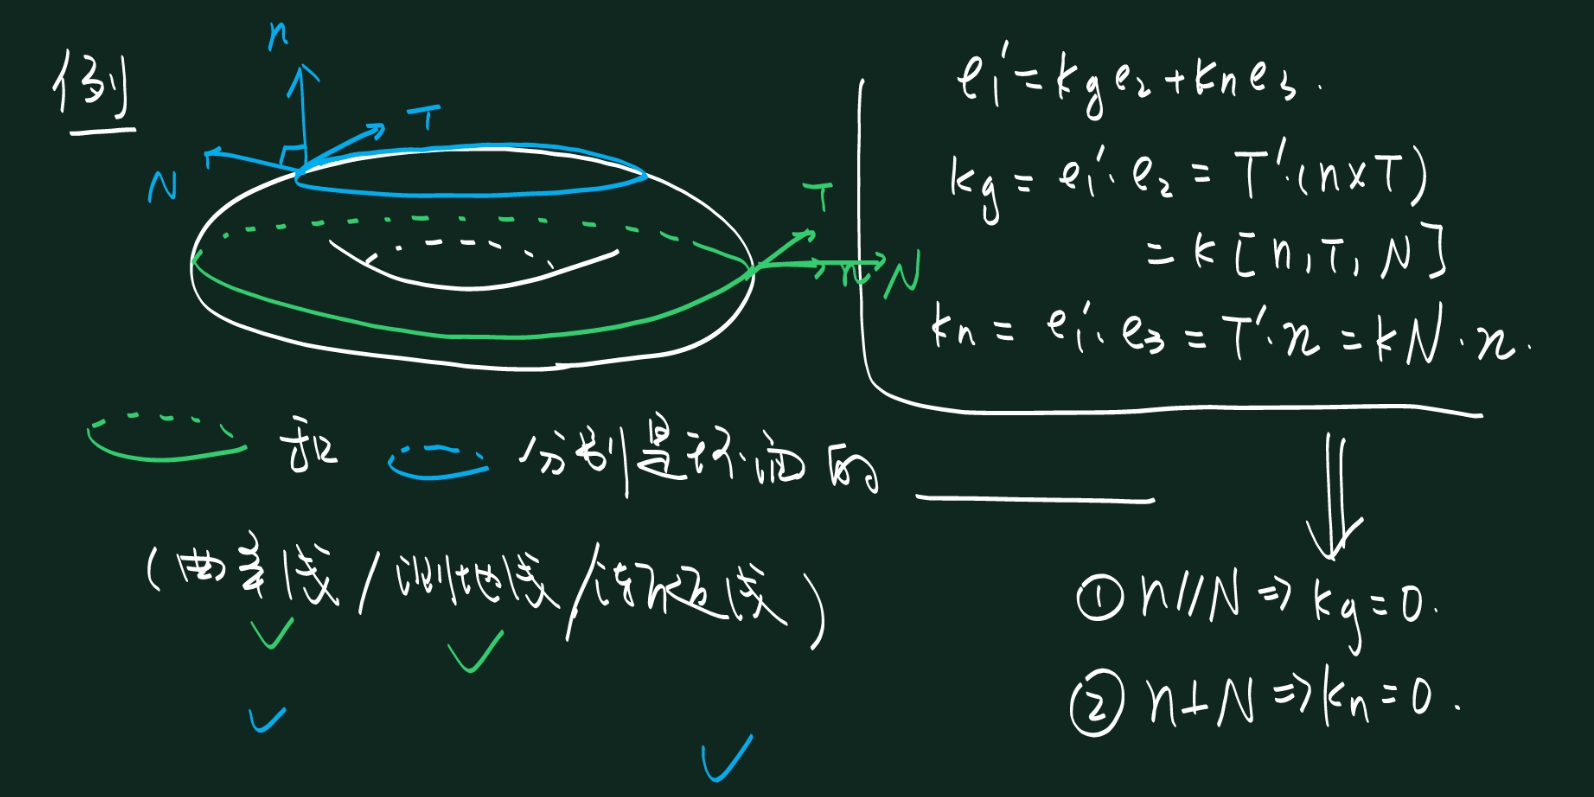
\includegraphics[width=0.8\textwidth]{figure/例题1.png}

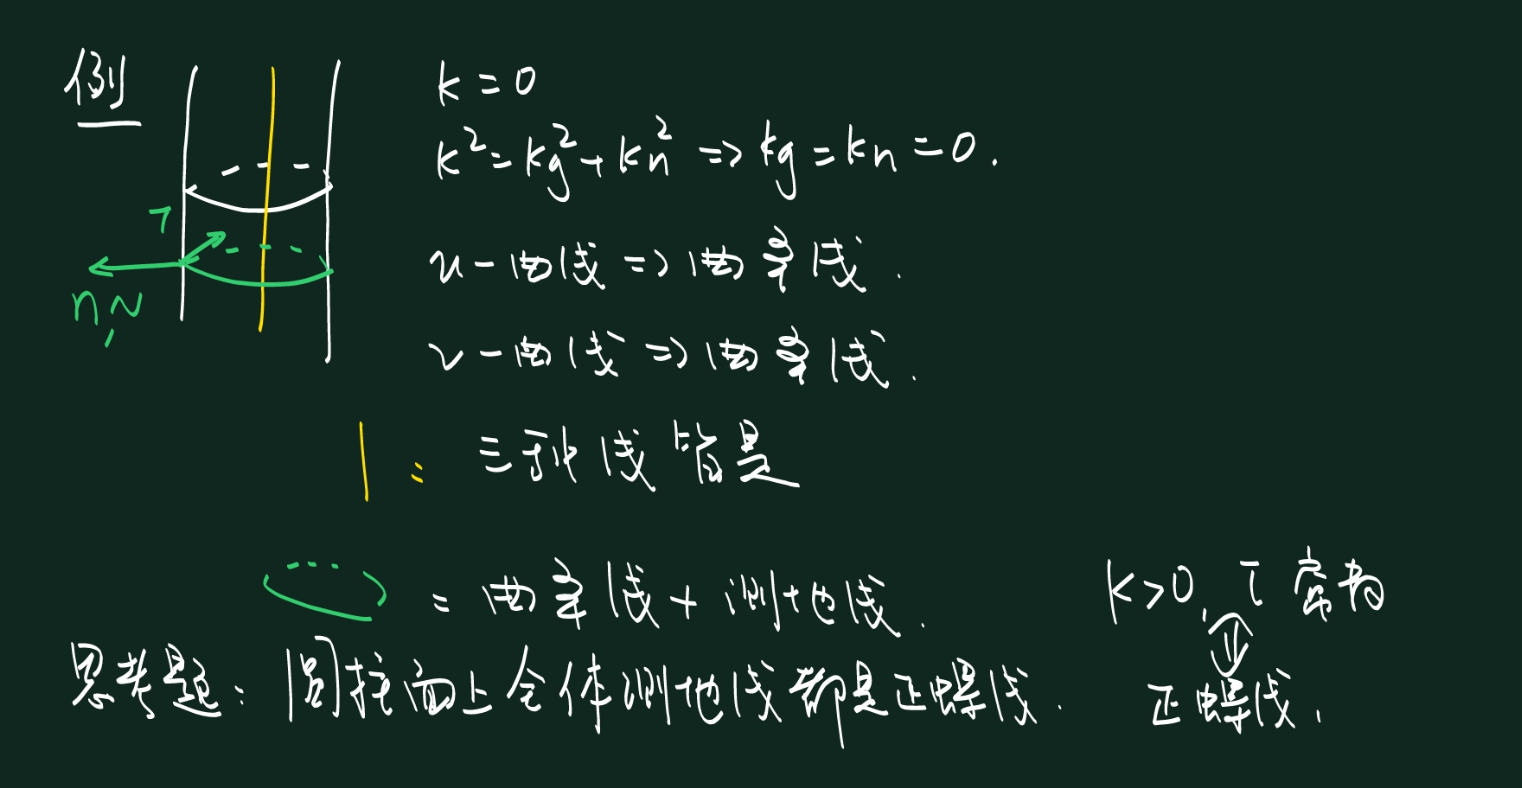
\includegraphics[width=0.8\textwidth]{figure/例题2.png}

\section{测地线的性质}
设 \( r(u^i(s), u^i(s)) \) 为测地线
\[
\Leftrightarrow \frac{d^2 u^k}{ds^2} + \Gamma^k_{ij} \frac{du^i}{ds} \frac{du^j}{ds} = 0.
\]
\begin{theorem}
    \(\forall p \in S, \forall v \in T_pS\),一定存在唯一的测地线
\[
r: (-\epsilon, \epsilon) \rightarrow S, \text{ 满足 } r(0) = p \text{ 且 } r'(0) = v.
\]
\end{theorem}
\begin{proof}
    待定以下函数,\( u^k(s) \) 和 \( v^k(s) \),\( k = 1, 2 \)。

    满足以下 ODE 方程组,
    \[
    \begin{cases}
    \frac{d u^k(s)}{ds} = v^k(s) \\
    \frac{d v^k(s)}{ds} = \Gamma^k_{ij} v^i(s) v^j(s)
    \end{cases}
    \]
    由 ODE 齐次方程组解的存在唯一性定理必然有唯一解,但需要验证 \( r(u^1(s), u^2(s)) \) 确定是以 \( s \) 为弧长参数的测曲线。
目标证明曲线以 \( s \) 为弧长参数,即 \( |r'(s)| = 1 \) 对所有 \( s \) 成立。


切向量表达式:
\[
r'(s) = \frac{\partial r}{\partial u^i} \frac{du^i}{ds} = \frac{dr}{ds}
\]
其模长平方为:
\[
|r'(s)|^2 = r'(s) \cdot r'(s) = g_{ij} \frac{du^i}{ds} \frac{du^j}{ds}
\]
其中 \( g_{ij} = \frac{\partial r}{\partial u^i} \cdot \frac{\partial r}{\partial u^j} \) 是度量张量。\\
定义辅助函数:
\[
h(s) = |r'(s)|^2 - 1 = g_{ij}(u(s)) \frac{du^i}{ds} \frac{du^j}{ds} - 1
\]
由初始条件 \( |r'(0)| = 1 \),有 \( h(0) = 0 \)。若证 \( h(s) \equiv 0 \),则结论成立。


对 \( h(s) \) 求导:
\[
\frac{dh}{ds} = \frac{d}{ds}\left(g_{ij} \frac{du^i}{ds} \frac{du^j}{ds}\right)
\]
展开导数:
\begin{align}
\frac{d}{ds}\left(g_{ij} \frac{du^i}{ds} \frac{du^j}{ds}\right) 
&= \frac{\partial g_{ij}}{\partial u^k} \frac{du^k}{ds} \frac{du^i}{ds} \frac{du^j}{ds} \notag \\
&+ g_{ij} \frac{d^2 u^i}{ds^2} \frac{du^j}{ds} \notag \\
&+ g_{ij} \frac{du^i}{ds} \frac{d^2 u^j}{ds^2} \label{eq:deriv}
\end{align}
利用 \( g_{ij} = g_{ji} \) 的对称性,可合并后两项:
\[
g_{ij} \frac{d^2 u^i}{ds^2} \frac{du^j}{ds} + g_{ij} \frac{du^i}{ds} \frac{d^2 u^j}{ds^2} = 2g_{ij} \frac{d^2 u^i}{ds^2} \frac{du^j}{ds}
\]

由测地线方程:
\[
\frac{d^2 u^i}{ds^2} = -\Gamma_{pq}^i \frac{du^p}{ds} \frac{du^q}{ds}
\]
代入式 (\ref{eq:deriv}) 的第二部分:
\[
2g_{ij} \frac{d^2 u^i}{ds^2} \frac{du^j}{ds} = 2g_{ij}\left( -\Gamma_{pq}^i \frac{du^p}{ds} \frac{du^q}{ds} \right) \frac{du^j}{ds} = -2\Gamma_{pqj} \frac{du^p}{ds} \frac{du^q}{ds} \frac{du^j}{ds}
\]
其中 \( \Gamma_{pqj} = g_{ij}\Gamma_{pq}^i \)。\\
对于第一部分,利用度量张量导数与Christoffel符号的关系:
\[
\frac{\partial g_{ij}}{\partial u^k} = \Gamma_{kij} + \Gamma_{kji}
\]
其中第一类Christoffel符号定义为:
\[
\Gamma_{kij} = \frac{1}{2}\left( \frac{\partial g_{kj}}{\partial u^i} + \frac{\partial g_{ik}}{\partial u^j} - \frac{\partial g_{ij}}{\partial u^k} \right)
\]
代入得:
\[
\frac{\partial g_{ij}}{\partial u^k} \frac{du^k}{ds} \frac{du^i}{ds} \frac{du^j}{ds} = (\Gamma_{kij} + \Gamma_{kji}) \frac{du^k}{ds} \frac{du^i}{ds} \frac{du^j}{ds}
\]

将两部分合并:
\begin{align*}
\frac{dh}{ds} &= (\Gamma_{kij} + \Gamma_{kji}) \frac{du^k}{ds} \frac{du^i}{ds} \frac{du^j}{ds} - 2\Gamma_{pqj} \frac{du^p}{ds} \frac{du^q}{ds} \frac{du^j}{ds} \\
&= \Gamma_{kij} \frac{du^k}{ds} \frac{du^i}{ds} \frac{du^j}{ds} + \Gamma_{kji} \frac{du^k}{ds} \frac{du^i}{ds} \frac{du^j}{ds} - 2\Gamma_{pqj} \frac{du^p}{ds} \frac{du^q}{ds} \frac{du^j}{ds}
\end{align*}
重命名哑指标(\( k \to p \), \( i \to q \), \( j \to j \)):
\[
\frac{dh}{ds} = \Gamma_{pqj} \frac{du^p}{ds} \frac{du^q}{ds} \frac{du^j}{ds} + \Gamma_{pjq} \frac{du^p}{ds} \frac{du^q}{ds} \frac{du^j}{ds} - 2\Gamma_{pqj} \frac{du^p}{ds} \frac{du^q}{ds} \frac{du^j}{ds}
\]
由Christoffel符号的对称性 \( \Gamma_{pjq} = \Gamma_{pqj} \):
\[
\frac{dh}{ds} = \Gamma_{pqj} \frac{du^p}{ds} \frac{du^q}{ds} \frac{du^j}{ds} + \Gamma_{pqj} \frac{du^p}{ds} \frac{du^q}{ds} \frac{du^j}{ds} - 2\Gamma_{pqj} \frac{du^p}{ds} \frac{du^q}{ds} \frac{du^j}{ds} = 0
\]


由 \( \frac{dh}{ds} \equiv 0 \) 和初始条件 \( h(0) = 0 \),根据微分方程解的唯一性,得:
\[
h(s) \equiv 0 \quad \forall s
\]
即:
\[
|r'(s)|^2 = g_{ij} \frac{du^i}{ds} \frac{du^j}{ds} = 1 \quad \Rightarrow \quad |r'(s)| = 1
\]
故曲线 \( r(s) = r(u^1(s), u^2(s)) \) 以 \( s \) 为弧长参数。

\end{proof}
\begin{proposition}
    平面上测地线 \(\Leftrightarrow\) 直线。
\end{proposition}
\begin{proof}
    平面 \( I = (1, 0, 0) \)。
\[
\Rightarrow \Gamma^k_{ij} = 0 \Rightarrow \text{测地线方程 } \frac{d^2 u^k}{ds^2} = 0.
\]
\[
\Rightarrow u^k \text{ 线性} \Rightarrow \text{测地线为直线} 
\]
\end{proof}

事实上,测地线是直线在曲面上的一种推广。

众所周知:平面上两点之间线段最短测地线有类似性质,它的弧长在变分下达到了极值。

下面介绍何为曲线在曲面上的变分
\[
(u^1(s), u^2(s)) \longrightarrow r(u^1(s), u^2(s)),
\]
扰动 \( u^1(s), u^2(s) \) 适当 \(\longrightarrow\) 给出一族曲面上的曲线

\begin{definition}[曲线在曲面上的变分]
    我们称 $\alpha^k: [a, b] \times (-\epsilon, \epsilon) \rightarrow \mathbb{R}^n$,\(k = 1, 2, \ldots\) 为 $u^k: [a, b] \rightarrow \mathbb{R}^n$ 的变分。

    若有 
    \begin{enumerate}
        \item $\alpha^k$ 关于 $t$ 连续,
        \item $\alpha^k(s, 0) = u^k(s)$。
    \end{enumerate}
    
    特别地,我们称其为一个定端变分,若 $\alpha^k(a, t) = u^k(a)$,$\alpha^k(b, t) = u^k(b)$。
    

\end{definition}
在定端变分下,我们也将
\[
r(u^1(s), u^2(s)) \longrightarrow r(s)
\]
\[
r(\alpha^1(s, t), \alpha^2(s, t)) \longrightarrow r_t(s) \text{ 一族头尾固定的曲线。}
\]
我们先记 \( v^k(s) = \left. \frac{d}{dt} \right|_{t=0} \alpha^k(s, t) \),称为变分方向。

\begin{proposition}[弧长变分公式]
\[
\left. \frac{d}{dt} \right|_{t=0} L(r_t) = -\int_a^b g_{ij} v^i \left( \frac{d^2 u^j}{ds^2} + \Gamma^j_{pq} \frac{du^p}{ds} \frac{du^q}{ds} \right) ds.
\]
\end{proposition}




\begin{proof}
    考虑曲线族 \( r_t(s) = r(s,t) \) 满足:
    \begin{itemize}
      \item \( r_0(s) = r(s,0) \) 是参考曲线(以弧长参数化)。
      \item 变分向量场 \( v^i(s) = \left. \frac{\partial u^i}{\partial t} \right|_{t=0} \)。
      \item 固定端点条件:\( v^i(a) = v^i(b) = 0 \)。
    \end{itemize}
    
    长度泛函定义为:
    \[
    L(r_t) = \int_a^b \left| \frac{\partial r}{\partial s} \right| ds = \int_a^b \sqrt{ g_{ij}(u(s,t)) \frac{\partial u^i}{\partial s} \frac{\partial u^j}{\partial s} }  ds.
    \]
    
    在参考曲线 (\( t=0 \)) 上计算变分。由于弧长参数化:
    \[
    \sqrt{ g_{ij} \frac{\partial u^i}{\partial s} \frac{\partial u^j}{\partial s} } \bigg|_{t=0} = 1,
    \]
    因此:
    \begin{align}
        \left. \frac{d}{dt} \right|_{t=0} L(r_t) 
        &= \int_a^b \left. \frac{d}{dt} \right|_{t=0} \sqrt{ g_{ij} \frac{\partial u^i}{\partial s} \frac{\partial u^j}{\partial s} }  ds \nonumber \\
        &= \frac{1}{2} \int_a^b \left. \frac{d}{dt} \right|_{t=0} \left( g_{ij} \frac{\partial u^i}{\partial s} \frac{\partial u^j}{\partial s} \right) ds \label{eq:main} \\
        &= \frac{1}{2} \int_a^b \left[ \left( \partial_k g_{ij} v^k \right) \frac{du^i}{ds} \frac{du^j}{ds} + 2g_{ij} \frac{du^j}{ds} \frac{\partial v^i}{\partial s} \right] ds, \nonumber
    \end{align}
    其中 \( \frac{du^i}{ds} = \left. \frac{\partial u^i}{\partial s} \right|_{t=0} \) 是参考曲线的切向量。
    
    对含 \( \frac{\partial v^i}{\partial s} \) 的项进行分部积分:
    \[
    \int_a^b g_{ij} \frac{du^j}{ds} \frac{\partial v^i}{\partial s}  ds = \left[ g_{ij} \frac{du^j}{ds} v^i \right]_a^b - \int_a^b \frac{\partial}{\partial s} \left( g_{ij} \frac{du^j}{ds} \right) v^i  ds.
    \]
    由固定端点条件 \( v^i(a) = v^i(b) = 0 \),边界项为零:
    \[
    \int_a^b g_{ij} \frac{du^j}{ds} \frac{\partial v^i}{\partial s}  ds = - \int_a^b \left( \partial_k g_{ij} \frac{du^k}{ds} \frac{du^j}{ds} + g_{ij} \frac{d^2 u^j}{ds^2} \right) v^i  ds. \label{eq:partial_int}
    \]
    
    将式 \eqref{eq:partial_int} 代入式 \eqref{eq:main}:
    \begin{align}
        \left. \frac{d}{dt} \right|_{t=0} L(r_t) 
        &= \frac{1}{2} \int_a^b \left[ \partial_k g_{ij} v^k \frac{du^i}{ds} \frac{du^j}{ds} - 2 \left( \partial_k g_{ij} \frac{du^k}{ds} \frac{du^j}{ds} + g_{ij} \frac{d^2 u^j}{ds^2} \right) v^i \right] ds \nonumber \\
        &= \frac{1}{2} \int_a^b v^i \left[ \partial_i g_{jk} \frac{du^j}{ds} \frac{du^k}{ds} - 2 \partial_j g_{ik} \frac{du^j}{ds} \frac{du^k}{ds} - 2 g_{ij} \frac{d^2 u^j}{ds^2} \right] ds. \label{eq:combined}
    \end{align}
    
    由 Christoffel 符号的定义(第一类):
    \[
    \Gamma_{ijk} = \frac{1}{2} \left( \partial_j g_{ik} + \partial_k g_{ij} - \partial_i g_{jk} \right),
    \]
    则式 \eqref{eq:combined} 中导数项的系数可表示为:
    \begin{align*}
        \partial_i g_{jk} - 2 \partial_j g_{ik} 
        &= \left[ -2 \Gamma_{ijk} + (\partial_j g_{ik} + \partial_k g_{ij} - \partial_i g_{jk}) \right] - 2 \partial_j g_{ik} \\
        &= -2 \Gamma_{ijk} - \partial_j g_{ik} + \partial_k g_{ij}.
    \end{align*}
    代入式 \eqref{eq:combined}:
    \begin{align*}
        \left. \frac{d}{dt} \right|_{t=0} L(r_t) 
        &= \frac{1}{2} \int_a^b v^i \left[ \left( -2 \Gamma_{ijk} - \partial_j g_{ik} + \partial_k g_{ij} \right) \frac{du^j}{ds} \frac{du^k}{ds} - 2 g_{ij} \frac{d^2 u^j}{ds^2} \right] ds \\
        &= \frac{1}{2} \int_a^b v^i \left[ -2 \Gamma_{ijk} \frac{du^j}{ds} \frac{du^k}{ds} - (\partial_j g_{ik} - \partial_k g_{ij}) \frac{du^j}{ds} \frac{du^k}{ds} - 2 g_{ij} \frac{d^2 u^j}{ds^2} \right] ds.
    \end{align*}
    由于 \( \partial_j g_{ik} - \partial_k g_{ij} \) 关于指标 \( j,k \) 反对称,而 \( \frac{du^j}{ds} \frac{du^k}{ds} \) 对称,其乘积为零:
    \[
    (\partial_j g_{ik} - \partial_k g_{ij}) \frac{du^j}{ds} \frac{du^k}{ds} = 0.
    \]
    因此:
    \[
    \left. \frac{d}{dt} \right|_{t=0} L(r_t) = \frac{1}{2} \int_a^b v^i \left[ -2 \Gamma_{ijk} \frac{du^j}{ds} \frac{du^k}{ds} - 2 g_{ij} \frac{d^2 u^j}{ds^2} \right] ds.
    \]
    
    将第一类 Christoffel 符号转换为第二类 \( \Gamma_{jk}^l = g^{lm} \Gamma_{jkm} \),并利用 \( \Gamma_{ijk} = g_{il} \Gamma_{jk}^l \):
    \begin{align*}
        \left. \frac{d}{dt} \right|_{t=0} L(r_t) 
        &= -\int_a^b v^i \left[ g_{il} \Gamma_{jk}^l \frac{du^j}{ds} \frac{du^k}{ds} + g_{il} \frac{d^2 u^l}{ds^2} \right] ds \\
        &= -\int_a^b g_{il} v^i \left( \frac{d^2 u^l}{ds^2} + \Gamma_{jk}^l \frac{du^j}{ds} \frac{du^k}{ds} \right) ds.
    \end{align*}
    重新标记哑指标 \( l \to j \),即得:
    \[
    \left. \frac{d}{dt} \right|_{t=0} L(r_t) = -\int_a^b g_{ij} v^i \left( \frac{d^2 u^j}{ds^2} + \Gamma^j_{pq} \frac{du^p}{ds} \frac{du^q}{ds} \right) ds.
    \]
    
    当参考曲线是测地线时,满足测地线方程:
    \[
    \frac{d^2 u^j}{ds^2} + \Gamma^j_{pq} \frac{du^p}{ds} \frac{du^q}{ds} = 0,
    \]
    因此:
    \[
    \left. \frac{d}{dt} \right|_{t=0} L(r_t) = 0,
    \]
    这表明测地线是长度泛函的临界点。
\end{proof}
\begin{corollary}
    若曲线为测地线 \(\Rightarrow \left. \frac{d}{dt} \right|_{t=0} L(r_t) = 0\)。
\end{corollary}

\begin{theorem}
    \( r(s) \) 是变分中的弧长达到极值的曲线 \(\Leftrightarrow r(s)\) 为测地线。
\end{theorem}
\begin{proof}
    \textbf{(\(\Leftarrow\))方向:} 若 \( r(s) \) 为测地线,则测地曲率 \( k_g = 0 \)。由变分法基本公式,弧长一阶变分为:
    \[
    \left. \frac{d}{dt} \right|_{t=0} L(r_t) = 0
    \]
    因此弧长达到临界值(极值条件)。
    
    \textbf{(\(\Rightarrow\))方向:} 若对任意变分 \( v_t \) 满足端点固定(即 \( v^k(a) = v^k(b) = 0 \)),都有:
    \[
    \left. \frac{d}{dt} \right|_{t=0} L(v_t) = 0
    \]
    构造特殊变分场:
    \[
    v^k(s) = \sin \left( \frac{\pi (s - a)}{b - a} \right) \left[ \frac{d^2 u^k}{ds^2} + \Gamma_{ij}^k \frac{du^i}{ds} \frac{du^j}{ds} \right]
    \]
    其中 \( u^k \) 是 \( r(s) \) 的局部坐标表示。易验证:
    \[
    v^k(a) = \sin(0) \cdot [\cdots] = 0, \quad v^k(b) = \sin(\pi) \cdot [\cdots] = 0
    \]
    满足端点条件。代入一阶变分公式得:
    \[
    0 = -\int_a^b \sin \left( \frac{\pi (s - a)}{b - a} \right) \cdot k_g^2  \dd s
    \]
    其中 \( k_g^2 = g_{kl} \left( \frac{d^2 u^k}{ds^2} + \Gamma_{ij}^k \frac{du^i}{ds} \frac{du^j}{ds} \right) \left( \frac{d^2 u^l}{ds^2} + \Gamma_{mn}^l \frac{du^m}{ds} \frac{du^n}{ds} \right) \) 是测地曲率平方。
    
    由于度量正定,\( k_g^2 \geq 0 \) 恒成立,且被积函数中:
    \[
    \sin \left( \frac{\pi (s - a)}{b - a} \right) > 0, \quad \forall s \in (a,b)
    \]
    因此有:
    \[
    \int_a^b \underbrace{\sin \left( \frac{\pi (s - a)}{b - a} \right)}_{>0} \cdot \underbrace{k_g^2}_{\geq 0}  \dd s = 0
    \]
    这要求 \( k_g^2 = 0 \) 在 \([a,b]\) 上几乎处处成立。由连续性,\( k_g(s) = 0 \) 对所有 \( s \in [a,b] \) 成立,故 \( r(s) \) 是测地线。
    
   
    \[
    k_g e_2 = \left( \frac{d^2 u^k}{ds^2} + \Gamma_{ij}^k \frac{du^i}{ds} \frac{du^j}{ds} \right) \vec{e}_k
    \]
    当 \( k_g = 0 \) 时,测地方程成立。
\end{proof}

\section{参数网}
事实上曲面每点处局部可选择特殊的参考。
(u, v) 使得在局部上计算变得简洁。
这件事情需要基于以下引理。

\begin{lemma}
    设 $f, g \in C^1(D)$,$D \subset \mathbb{R}^2$,$\forall p \in D$,在 $U \subset D$ 使得总存在 $F \in C^1(D)$ 和 $\lambda \in C(U)$,使
\[
dF = \lambda (f \, du + g \, dv).
\]
\end{lemma}

\begin{lemma}
    设 $r: D \rightarrow \mathbb{R}^3$ 为正则曲面,\(a(u,v)\) 和 \(b(u,v)\) 是 \(D\) 上的两个向量场(切向量的分布)。

(即 \(\forall (u_0,v_0) \in D\),\(a(u_0,v_0) \in T_{(u_0,v_0)}S\)。)
那么 \(\forall p \in D\),总是存在 \(p \in U \subseteq D\) 使得在 \(U\) 上可取到新参数 \((\widetilde{u}, \widetilde{v})\) 

满足 \(r_{\widetilde{u}} \parallel a\),\(r_{\widetilde{v}} \parallel b\),\(\forall (u,v) \in U\)。
\end{lemma}

\begin{proof}
    在每点 \( T_{(u,v)}S \) 上,总有 \( a_1(u,v) \) 和 \( a_2(u,v) \) 正交,
\[
\text{使 } a(u,v) = a_1(u,v) r_u(u,v) + a_2(u,v) r_v(u,v).
\]
以下简记为
\[
a = a_1 r_u + a_2 r_v.
\]
同理有
\[
b = b_1 r_u + b_2 r_v.
\]
定义矩阵 \( A = \begin{bmatrix} a_1 & a_2 \\ b_1 & b_2 \end{bmatrix} \),则 \( a, b \) 线性无关当且仅当
\[
\det A = a_1 b_2 - a_2 b_1 \neq 0, \quad \forall (u,v) \in D.
\]

由引理可知,\(\forall p \in D\),一定存在邻域 \( p \in U \subseteq D \),在 \( U \) 上有 \(\widetilde{u}, \widetilde{v} \in C^1(U)\) 和函数 \(\lambda, \mu \in C(U)\),使得
\[
\begin{cases}
d\widetilde{u} = \lambda (b_2 du - b_1 dv) \\
d\widetilde{v} = \mu (-a_2 du + a_1 dv)
\end{cases}
\]
并满足
\[
r_{\widetilde{u}} \parallel a, \quad r_{\widetilde{v}} \parallel b.
\]

容易看出,坐标变换的 Jacobi 矩阵为
\[
\frac{\partial (\widetilde{u}, \widetilde{v})}{\partial (u,v)} = \begin{bmatrix} \widetilde{u}_u & \widetilde{u}_v \\ \widetilde{v}_u & \widetilde{v}_v \end{bmatrix} = \begin{bmatrix} \lambda b_2 & -\lambda b_1 \\ -\mu a_2 & \mu a_1 \end{bmatrix}.
\]
其逆矩阵为
\[
\frac{\partial (u,v)}{\partial (\widetilde{u}, \widetilde{v})} = \frac{1}{\lambda \mu \det A} \begin{bmatrix} \mu a_1 & \lambda b_1 \\ \mu a_2 & \lambda b_2 \end{bmatrix}.
\]
于是
\[
r_{\widetilde{u}} = \frac{\partial u}{\partial \widetilde{u}} r_u + \frac{\partial v}{\partial \widetilde{u}} r_v = \frac{1}{\lambda \det A} (a_1 r_u + a_2 r_v) = \frac{1}{\lambda \det A} a \implies r_{\widetilde{u}} \parallel a.
\]
同理,
\[
r_{\widetilde{v}} = \frac{\partial u}{\partial \widetilde{v}} r_u + \frac{\partial v}{\partial \widetilde{v}} r_v = \frac{1}{\mu \det A} (b_1 r_u + b_2 r_v) = \frac{1}{\mu \det A} b \implies r_{\widetilde{v}} \parallel b.
\]
\end{proof}
\subsection{正交参数网(局部上F=0)}
对于任意的 $(u,v)$ 参数,作 Schmit 正交化。

令 $e_1 = \frac{r_u}{\sqrt{E}}$ 单位向量。

令 $b = r_v - \lambda e_1$,要求 $b \cdot e_1 = 0$,算 $\lambda$。
\[
\Rightarrow (r_v - \lambda e_1) \cdot e_1 = 0 \Rightarrow \lambda = r_v \cdot e_1 = r_v \cdot \frac{r_u}{\sqrt{E}} = \frac{F}{\sqrt{E}}.
\]
\[
\Rightarrow b = r_v - \frac{F}{E} r_u.
\]
\[
b \cdot b = G - \frac{2E^2}{E} + \frac{F^2}{E} = G - \frac{F^2}{E} = \frac{EG - F^2}{E}.
\]

令 $e_2 = \frac{b}{|b|} = \frac{r_v - \frac{F}{E} r_u}{\sqrt{EG - F^2 / E}}$。

$\{e_1, e_2\}$ 单位正交向量场。

由引理可知,局部上总有 $(\widetilde{u}, \widetilde{v})$ 正交参数,
\[
\text{使 } r_{\widetilde{u}} \parallel e_1, \quad r_{\widetilde{v}} \parallel e_2.
\]
\[
\Rightarrow \text{在 } (\widetilde{u}, \widetilde{v}) \text{ 坐标下 } F \text{ 局部恒为 } 0.
\]
我们称这样的 $(\widetilde{u}, \widetilde{v})$ 是正交网。
\subsection{曲率线参数网(局部上 \(F = M = 0\))}
假设 $P$ 是 $S$ 上的非脐点(脐点 $k_1 = k_2$)。

那么我们可取 $k_1$ 和 $k_2$ 对应的特征方向 $v_1, v_2$。

$(k_1, k_2$ 是 $C^1$ 的。$\left\{
\begin{array}{l}
k = k_1 \cdot k_2 \\
H = \frac{k_1 + k_2}{2}
\end{array}
\right. \Rightarrow v_1, v_2$ 是两个 $C'$、线性无关向量场)

自然局部上可取到 $(\widetilde{u}, \widetilde{v})$ 使得 $r_{\widetilde{u}} \parallel v_1$,$r_{\widetilde{v}} \parallel v_2$。

注意到 $v_1 \perp v_2$(两个特征值的特征方向)。

$\Rightarrow \widetilde{F} = 0$。取 $\omega$ 为 Weingarten 算子。

\[
\Rightarrow
\left\{
\begin{array}{l}
\omega(r_{\widetilde{u}}) = -n_{\widetilde{u}} = k_1 r_{\widetilde{u}} \cdot \\
\omega(r_{\widetilde{v}}) = -n_{\widetilde{v}} = k_2 r_{\widetilde{v}}
\end{array}
\right.
\left(
\begin{array}{l}
\omega(v_1) = k_1 v_1 \\
\omega(v_2) = k_2 v_2
\end{array}
\right)
\]

\[
\Rightarrow
\left\{
\begin{array}{l}
\widetilde{L} = -n_{\widetilde{u}} \cdot r_{\widetilde{u}} = k_1 r_{\widetilde{u}} \cdot r_{\widetilde{u}} = k_1 \widetilde{E} \\
\widetilde{M} = -n_{\widetilde{u}} \cdot r_{\widetilde{v}} = k_1 r_{\widetilde{u}} \cdot r_{\widetilde{v}} = 0 \\
\widetilde{N} = -n_{\widetilde{v}} \cdot r_{\widetilde{v}} = k_2 r_{\widetilde{v}} \cdot r_{\widetilde{v}} = k_2 \widetilde{G}
\end{array}
\right.
\]

若用曲率线网,则局部上
\[
I= E \, du \otimes du + G \, dv \otimes dv
\]
而
\[
II = k_1 E \, du \otimes du + k_2 G \, dv \otimes dv.
\]

\begin{example}
    设 $S$ 为已测曲面,$P$ 为其上的非脐点。

    \begin{enumerate}
        \item 设 $r(s)$ 过 $P$ 以 $S$ 为弧长的一条曲面上曲线,$\theta$ 为对应的切向角,则有以下公式:
        \[
        \tau_g = (k_2 - k_1) \sin \theta \cos \theta.
        \]

        \item 证明:若过 $P$ 可作两条渐近线,则
        \[
        \tau_{g_1} = -\tau_{g_2}.
        \]

        \item 证明:$\tau_{g_1} \cdot \tau_{g_2} = K_p$。(CMC原题)
    \end{enumerate}

\end{example}
\begin{proof}
    (1)给定第一基本形式和第二基本形式:
    \[
    I = E  du^2 + 2F  du  dv + G  dv^2, \quad II = L  du^2 + 2M  du  dv + N  dv^2
    \]
    曲线切向量表示为:
    \[
    r'(s) = \frac{du}{ds} \mathbf{r}_u + \frac{dv}{ds} \mathbf{r}_v = \left( \frac{du}{ds} \sqrt{E} \right) \frac{\mathbf{r}_u}{\sqrt{E}} + \left( \frac{dv}{ds} \sqrt{G} \right) \frac{\mathbf{r}_v}{\sqrt{G}}
    \]
    其中单位切向分量满足:
    \[
    \frac{du}{ds} \sqrt{E} = \cos \theta, \quad \frac{dv}{ds} \sqrt{G} = \sin \theta
    \]
    即:
    \[
    \frac{du}{ds} = \frac{\cos \theta}{\sqrt{E}}, \quad \frac{dv}{ds} = \frac{\sin \theta}{\sqrt{G}}
    \]
    \[
    \tau_g = (k_2 - k_1) \sin \theta \cos \theta
    \]

    (2)由 Euler 公式:
    \[
    k_n = k_1 \cos^2 \theta + k_2 \sin^2 \theta = 0
    \]
    解得:
    \[
    \tan^2 \theta = -\frac{k_1}{k_2} \quad (\text{要求 } k_1 k_2 < 0 \text{,即 } P \text{ 为双曲点})
    \]
    对两条曲线,有 \( \tan^2 \theta_1 = \tan^2 \theta_2 \),故:
    \[
    \theta_1 = -\theta_2 \quad (\text{方向相反})
    \]
    由测地曲率公式:
    \[
    \tau_{g1} = (k_2 - k_1) \sin \theta_1 \cos \theta_1, \quad \tau_{g2} = (k_2 - k_1) \sin(-\theta_1) \cos(-\theta_1) = -(k_2 - k_1) \sin \theta_1 \cos \theta_1
    \]
    因此:
    \[
    \tau_{g1} = -\tau_{g2}
    \]

    (3)由 (2) 知 \( T_{g2} = -T_{g1} \),且两条曲线均为渐近曲线(\( k_n = 0 \))。  
    计算乘积:
    \[
    \tau_{g1} \tau_{g2} = \tau_{g1} (-\tau_{g1}) = -\tau_{g1}^2 = - \left[ (k_2 - k_1) \sin \theta_1 \cos \theta_1 \right]^2 = - (k_2 - k_1)^2 \sin^2 \theta_1 \cos^2 \theta_1
    \]
    由 Euler 公式 \( k_n = 0 \) 导出关系:
    \begin{align*}
    k_1 \cos^2 \theta_1 + k_2 \sin^2 \theta_1 &= 0 \\
    \Rightarrow k_1 &= -(k_2 - k_1) \sin^2 \theta_1 \\
    k_2 &= (k_2 - k_1) \cos^2 \theta_1
    \end{align*}
    代入乘积式:
    \[
    - (k_2 - k_1)^2 \sin^2 \theta_1 \cos^2 \theta_1 = - \left[ (k_2 - k_1) \sin^2 \theta_1 \right] \left[ (k_2 - k_1) \cos^2 \theta_1 \right] = - \left[ -k_1 \right] \left[ k_2 \right] = k_1 k_2
    \]
    高斯曲率 \( K_p = k_1 k_2 \),故:
    \[
    \tau_{g1} \tau_{g2} = K_p
    \]
\end{proof}
\begin{example}
    $\mathbf{III} = dn \cdot dn$ 满足恒等式。
\[
\mathbf{III} - 2H\mathbf{II} + k\mathbf{I} = 0.
\]
\end{example}
\begin{proof}
    公式可逐项证明,故而可逐项取曲率线网。
\[
\mathbf{I} = E \, du \otimes du + G \, dv \otimes dv
\]
\[
\mathbf{II} = k_1 E \, du \otimes du + k_2 G \, dv \otimes dv
\]
\[
\mathbf{III} = k_1^2 E \, du \otimes du + k_2^2 G \, dv \otimes dv.
\]
\[
e = n_u \cdot n_u = k_1^2 E, \quad f = 0, \quad g = k_2^2 G \, dv \otimes dv.
\]
    直接验证即可
\end{proof}


\begin{theorem}
    平面上两点之间可微曲线之中线段最短。
\end{theorem}
\begin{proof}
    设 $P, Q \in \Sigma$,以 $P$ 为原点建立极坐标系 $(\rho, \theta)$。

\[
r(x, y) = (x, y, 0) = (\rho \cos \theta, \rho \sin \theta, 0).
\]
\[
r_{\rho} = (\cos \theta, \sin \theta, 0), \quad r_{\theta} = (-\rho \sin \theta, \rho \cos \theta, 0).
\]
\[
E = 1, \quad F = 0, \quad G = \rho^2.
\]
\[
I = d\rho \otimes d\rho + \rho^2 d\theta \otimes d\theta.
\]

设 $r: [0,1] \rightarrow \Sigma$ 为连接 $P, Q$ 的任意曲线。
\[
r(0) = P, \quad r(1) = Q, \quad r'(t) = \frac{d\rho}{dt} r_{\rho} + \frac{d\theta}{dt} r_{\theta}.
\]
\[
L(\widehat{PQ}) = \int_0^1 \left| \frac{dr}{dt} \right| dt = \int_0^1 \sqrt{\left( \frac{d\rho}{dt} \right)^2 + \rho^2 \left( \frac{d\theta}{dt} \right)^2} dt.
\]
\[
\geq \int_0^1 \frac{d\rho}{dt} dt = (\rho(1) - \rho(0)).\text{P 到 Q 的距离}.
\]
\[
\text{等号成立当且仅当 } \frac{d\theta}{dt} = 0 \Rightarrow \theta \text{ 常数} \Rightarrow \text{线段}.
\]

\end{proof}
我们希望仿照平面的极坐标给出曲面上的“极坐标系”。
\begin{definition}[指数映射]
    $\forall p \in S$.
\[
\exp_p: T_pS \longrightarrow S.
\]
\[
\sim \longmapsto r_v(1).
\]
我们之前证明过,$\forall p \in S$,$\forall v \in T_pM$,局部上总有测地线 $r_v(t)$ 满足 $r_v(0) = p$,$r_v'(0) = v$。
\end{definition}
\begin{lemma}\label{lemma}
    \( r_v(s) = r_{\frac{v}{\rho}}(\rho s) \), \(\forall \rho > 0 \in \mathbb{R}\).
\end{lemma}
\begin{proof}
    曲线形状一致,且
    \begin{enumerate}
        \item \(\displaystyle r_{\frac{v}{\rho}}(0) = \rho\).
        \item \(\displaystyle r'_{\frac{v}{\rho}}(0) = \rho \cdot \frac{v}{\rho} = v\).
    \end{enumerate}
    
    \textbf{由唯一性可知}
    \[
    r_v(s) = r_{\frac{v}{\rho}}(\rho s)
    \]
\end{proof}

\textbf{FACT} \quad \( r_v(s) = \exp_{\rho}(sv) \).
\begin{proof}
    \(\exp_{\rho}(sv) = r_{sv}(1)\) 引理\ref{lemma} \(r_v(s)\) \(\downarrow\)
\end{proof}


\textbf{FACT} \(\left. \frac{d}{ds} \right|_{s=0} \exp_{\rho}(sv) = \left. \frac{d}{ds} \right|_{s=0} r_v(s) = r'_v(0) = v\).





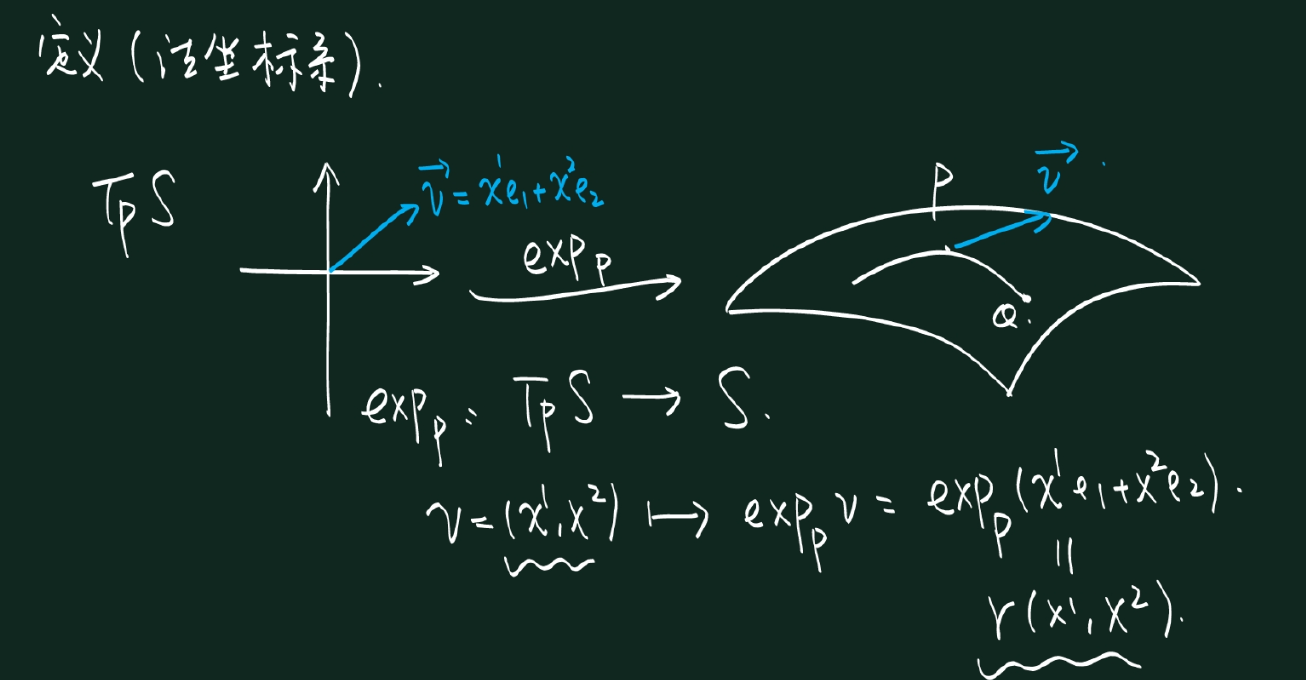
\includegraphics[width=0.8\textwidth]{figure/法坐标系.png}

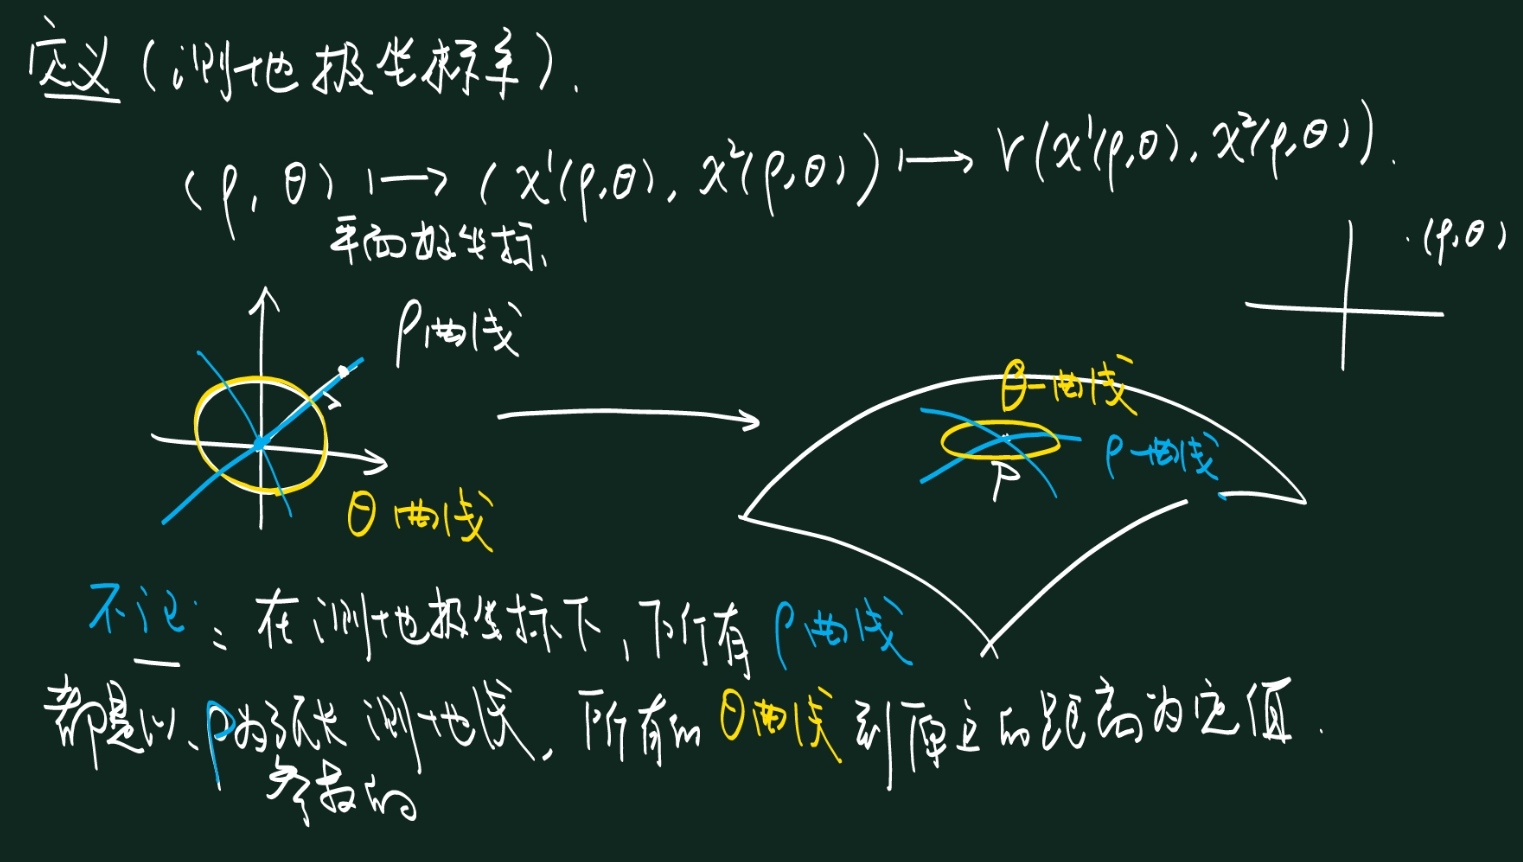
\includegraphics[width=0.8\textwidth]{figure/测地坐标系.png}


这个没图不行,直接给图了


\begin{lemma}[Gauss 引理]
    在曲面测地极坐标系中,\(\forall P\) 曲线都彼此正交。
\end{lemma}
\begin{proof}
    设曲面参数化为 \( r(\rho, \theta) \),其中:
\begin{align*}
r_\rho &= \frac{\partial r}{\partial \rho} = r_1 \cos \theta + r_2 \sin \theta \\
r_\theta &= \frac{\partial r}{\partial \theta} = \rho (-r_1 \sin \theta + r_2 \cos \theta)
\end{align*}
其中 \( r_1 = \frac{\partial r}{\partial u^1} \), \( r_2 = \frac{\partial r}{\partial u^2} \) 是坐标基向量。

\begin{enumerate}
    \item \begin{align*}
        F(\rho, \theta) &= r_\rho \cdot r_\theta \\
        &= (r_1 \cos \theta + r_2 \sin \theta) \cdot \rho (-r_1 \sin \theta + r_2 \cos \theta) \\
        &= \rho \left[ \cdots \right] \quad \text{(点积展开)}
        \end{align*}
        当 \(\rho \to 0\) 时(即趋向极点),有:
        \[
        \lim_{\rho \to 0} F(\rho, \theta) = 0.
        \]
    
    \item 计算 \( F \) 对 \(\rho\) 的偏导数:
    \begin{align*}
    \frac{\partial F}{\partial \rho} &= \frac{\partial}{\partial \rho} (r_\rho \cdot r_\theta) \\
    &= r_{\rho\rho} \cdot r_\theta + r_\rho \cdot r_{\rho\theta}
    \end{align*}
    其中 \( r_{\rho\rho} = \frac{\partial^2 r}{\partial \rho^2} \), \( r_{\rho\theta} = \frac{\partial^2 r}{\partial \rho \partial \theta} \).
    
    由曲面理论,二阶导数可用 Christoffel 符号表示:
    \[
    r_{\rho\rho} = \Gamma_{11}^1 r_\rho + \Gamma_{11}^2 r_\theta
    \]
    但关键性质是:\(\rho\)-曲线是测地线,且以 \(\rho\) 为弧长参数。测地线方程给出:
    \[
    \frac{d^2 u^k}{d\rho^2} + \Gamma_{ij}^k \frac{du^i}{d\rho} \frac{du^j}{d\rho} = 0
    \]
    对于 \(\rho\)-曲线(固定 \(\theta\)),有 \( du^1/d\rho = \cos \theta \), \( du^2/d\rho = \sin \theta \),且 \( d^2 u^k/d\rho^2 = 0 \)。代入得:
    \[
    \Gamma_{11}^k \cos^2 \theta + 2\Gamma_{12}^k \cos\theta \sin\theta + \Gamma_{22}^k \sin^2 \theta = 0
    \]
    特别地,当坐标系在极点正则时,有 \(\Gamma_{11}^k = 0\).
    
    同时,由弧长参数化条件:
    \[
    |r_\rho|^2 = 1 \implies \frac{\partial}{\partial \theta} (|r_\rho|^2) = 2 r_\rho \cdot r_{\rho\theta} = 0
    \]
    因此:
    \[
    \frac{\partial F}{\partial \rho} = (\Gamma_{11}^1 r_\rho + \Gamma_{11}^2 r_\theta) \cdot r_\theta + \frac{1}{2} \frac{\partial}{\partial \theta} (|r_\rho|^2) = 0
    \]
    故 \( F \) 与 \(\rho\) 无关,为常数。
\end{enumerate}

由边界条件:
\[
\lim_{\rho \to 0} F(\rho, \theta) = 0
\]
且 \( F \) 是常数,故对任意 \(\rho > 0\),
\[
F(\rho, \theta) = r_\rho \cdot r_\theta = 0
\]
正交性得证。
\end{proof}
\begin{proposition}
    法坐标系满足以下性质:
\begin{enumerate}
    \item \( g_{ij}(0,0) = \delta_{ij} \) \quad (即 \( P \) 点处的第一基本形式为 \( E_2 \))
    \item \( \Gamma^k_{ij}(0,0) = 0, \quad \forall i,j,k \).
\end{enumerate}
\end{proposition}
\begin{proof}
    \begin{enumerate}
        \item \( r(x^1, x^2) = \exp_{\rho}(x^1 e_1 + x^2 e_2) \)
        \[
        \left. \frac{\partial r}{\partial x^i} \right|_{(0,0)} = \left. \frac{d}{dx^i} \right|_{x^i=0} \exp_{\rho}(x^1 e_1) = \left. \frac{d}{dt} \right|_{t=0} \exp_{\rho}(t e_i) = e_i
        \]
        同理 \(\left. \frac{\partial r}{\partial x^2} \right|_{(0,0)} = e_2\),由 \(e_1, e_2\) 单位正交 \(\Rightarrow g_{ij}(0,0) = \delta_{ij}\)。
        \item 注意在测地极坐标系下,\(r(\rho, \theta)\) 的 \(\rho\)-曲线为测地线:$ \left\{
            \begin{array}{l}
            x^1 = \rho \cos \theta \\
            x^2 = \rho \sin \theta
            \end{array}
            \right.$
        \[
        \text{测地线方程:} \quad \frac{d^2 x^k}{d\rho^2} + \Gamma^k_{ij} \frac{dx^i}{d\rho} \frac{dx^j}{d\rho} = 0.
        \]
        \[
        r(x^1(\rho), x^2(\rho)) \quad \Rightarrow \quad \Gamma^k_{ij} f(\theta) = 0, \quad \forall \theta \quad \Rightarrow \quad \Gamma^k_{ij} = 0.
        \]
       
    \end{enumerate}
    
\end{proof}
\begin{proposition}
    测地极坐标一定满足以下性质。

\begin{enumerate}
    \item $I = d\rho \otimes d\rho + G(\rho, \theta) d\theta \otimes d\theta.$ ($E = 1, F = 0$).(Gauss 引理)
    \item $\lim_{\rho \to 0} \sqrt{G} = 0.$ (对照欧氏公式 $G = \rho^2$).
    \item $\lim_{\rho \to 0} \frac{\partial}{\partial \rho} \sqrt{G} = 1.$
    \item $K = \frac{-(\sqrt{G})_{\rho\rho}}{\sqrt{G}}$
\end{enumerate}
\end{proposition}
\begin{proof}
    \begin{enumerate}
        \item \begin{itemize}
            \item \( E = 1 \):因为 \(\rho\) 是径向测地线的弧长参数,故
            \[
            \left| \frac{\partial r}{\partial \rho} \right| = 1 \implies E = \left| r_\rho \right|^2 = 1.
            \]
            \item \( F = 0 \):由 Gauss 引理(前文已证明),在测地极坐标系中,径向与纬向曲线正交:
            \[
            r_\rho \cdot r_\theta = 0 \implies F = 0.
            \]
        \end{itemize}
        \item  考虑曲面在原点附近的参数化。设 \( x = \rho \cos \theta \), \( y = \rho \sin \theta \),则:
        \[
        r(\rho, \theta) = r(x(\rho, \theta), y(\rho, \theta))
        \]
        坐标变换的 Jacobian 行列式为:
        \[
        \left| \frac{\partial (x, y)}{\partial (\rho, \theta)} \right| = \begin{vmatrix}
        \cos \theta & -\rho \sin \theta \\
        \sin \theta & \rho \cos \theta
        \end{vmatrix} = \rho (\cos^2 \theta + \sin^2 \theta) = \rho
        \]
        面积元关系为:
        \[
        dA = \sqrt{EG - F^2}  dx  dy = \sqrt{G}  d\rho  d\theta
        \]
        又
        \[
        dx  dy = \left| \frac{\partial (x, y)}{\partial (\rho, \theta)} \right| d\rho  d\theta = \rho  d\rho  d\theta
        \]
        故
        \[
        \sqrt{EG - F^2} \cdot \rho  d\rho  d\theta = \sqrt{G}  d\rho  d\theta
        \]
        即
        \[
        \sqrt{G} = \rho \cdot \sqrt{EG - F^2}
        \]
        当 \(\rho \to 0\) 时:
        \[
        \lim_{\rho \to 0} \sqrt{G} = \lim_{\rho \to 0} \rho \cdot \sqrt{EG - F^2} = 0 \cdot \sqrt{1 \cdot 1 - 0} = 0
        \]

        \item 由上式:\[
\sqrt{G} = \rho \cdot h(\rho, \theta)
\]
其中 \( h(\rho, \theta) = \sqrt{EG - F^2} \) 是光滑函数,且在极点:
\[
h(0, \theta) = \sqrt{E(0,\theta)G(0,\theta) - F^2(0,\theta)} = \sqrt{1 \cdot 1 - 0} = 1
\]
则
\[
\frac{\partial}{\partial \rho} \sqrt{G} = h(\rho, \theta) + \rho \frac{\partial h}{\partial \rho}
\]
取极限 \(\rho \to 0\):
\[
\lim_{\rho \to 0} \frac{\partial}{\partial \rho} \sqrt{G} = h(0, \theta) + 0 \cdot \frac{\partial h}{\partial \rho} = 1
\]

        \item \[
        I = d\rho \otimes d\rho + G \, d\theta \otimes d\theta.
        \] 
        当 \( F = 0 \) 时可以用以下公式:
        \[
        K = -\frac{1}{\sqrt{EG}} \left\{ \left[ \frac{(\sqrt{E})_v}{\sqrt{G}} \right]_v + \left[ \frac{(\sqrt{G})_u}{\sqrt{E}} \right]_u \right\} \quad \sqrt{E} = 1, \quad \sqrt{G}, \quad u = \rho, \quad v = \theta.
        \]
        \[
        \Rightarrow K = -\frac{1}{\sqrt{G}} (\sqrt{G})_{\rho\rho}.
        \]
        
    \end{enumerate}
\end{proof}
可以利用(4)证明以下定理
\begin{theorem}
    所有 \( K \) 为常数的曲面彼此局部上保长对应,即第一基本形式一致
\end{theorem}
\begin{remark}
    \( K \) 非常数不对!
\end{remark}
\begin{proof}
    在局部上可建立测地极坐标系,\( u \)。

在 \( u \) 中有 \(  = -\frac{(\sqrt{G})_{\rho\rho}}{\sqrt{G}} \)。

\[
\Rightarrow \sqrt{G} \text{ 满足 ODE: } (\sqrt{G})_{\rho\rho} + K \sqrt{G} = 0.
\]
\begin{itemize}
    \item (情况一) \( K = 0 \)。\(\Rightarrow (\sqrt{G})_{\rho\rho} = 0\)。

\[
\Rightarrow (\sqrt{G})_{\rho} = f(\theta) \Rightarrow \sqrt{G} = \rho f(\theta) + g(\theta).
\]

但注意到
\begin{enumerate}
    \item \(\lim_{\rho \to 0} \sqrt{G} = 0 \Rightarrow g(\theta) = 0\).
    \item \(\lim_{\rho \to 0} \frac{\partial}{\partial \rho} \sqrt{G} = 1 \Rightarrow f(\theta) = 1 \Rightarrow \sqrt{G} = \rho \Rightarrow G = \rho^2\).
\end{enumerate}

和平面保长。
    \item (情况二)\( K = \frac{1}{a^2} > 0 \)。

    \[
    \Rightarrow (\sqrt{G})_{\rho\rho} + \frac{1}{a^2} \sqrt{G} = 0.
    \]
    
    通解为 \(\sqrt{G} = f(\theta) \cos \frac{\rho}{a} + g(\theta) \sin \frac{\rho}{a}\)。
    
    但注意到
    \begin{enumerate}
        \item \(\lim_{\rho \to 0} \sqrt{G} = 0 \Rightarrow f(\theta) = 0\).
        \item \(\lim_{\rho \to 0} \frac{\partial}{\partial \rho} \sqrt{G} = 1 \Rightarrow g(\theta) = 1 \Rightarrow \sqrt{G} = \sin \frac{\rho}{a}\).
    \end{enumerate}
    
    \[
    \Rightarrow I = d\rho \otimes d\rho + \sin^2 \frac{\rho}{a} d\theta \otimes d\theta.
    \]和球面保长
\item (情况三)\( K = -\frac{1}{a^2} < 0 \)。

\[
\Rightarrow I = d\rho \otimes d\rho + \sinh^2 \frac{\rho}{a} d\theta \otimes d\theta.
\]
无论哪种情况,\( I \) 都完全确定了,所以局部上保长    
\end{itemize}
\end{proof}
\begin{theorem}[测地线的局部最短性]
    在 \( P \) 处找一个邻域 \( U \),使得 \( U \) 上可以以 \( P \) 为原点建立测地极坐标系,若 \( Q \in U \),则 \( PQ \) 之间的测地线是所有曲面上连接 \( P \) 和 \( Q \) 的曲线中的最短曲线。
\end{theorem}
\begin{proof}
    设在极坐标系中 \( P \leftrightarrow \rho = 0, \quad Q = (\rho_0, \theta_0) \)。

\( PQ \) 间的测地线记为 \( \overline{C} \),由局部测地线唯一 \(\Rightarrow \overline{C}\) 即为 \( \rho \) 曲线

\[
\Rightarrow L(\overline{C}) = \rho_0.
\]
\begin{enumerate}
    \item 设 \( r \) 为完全落在 \( U \) 中连接 \( P \) 和 \( Q \) 的曲线。
    \begin{figure}[h]
        \centering
        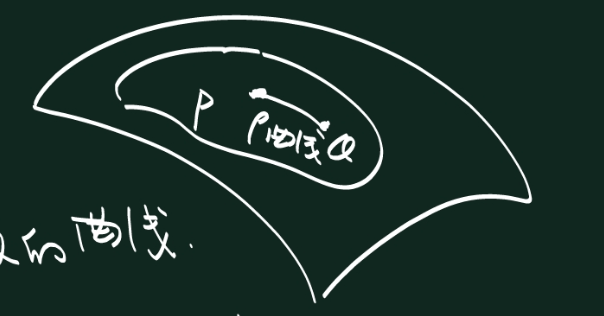
\includegraphics[width=0.48\textwidth]{fig1.png} % 图片宽度略小于环境宽度
    \end{figure}
    \[
    \frac{dr}{ds} = r_{\rho} \cdot \frac{d\rho}{ds} + r_{\theta} \cdot \frac{d\theta}{ds}
    \]
    \[
    \Rightarrow \left| \frac{dr}{ds} \right| = \sqrt{\left( \frac{d\rho}{ds} \right)^2 + G \left( \frac{d\theta}{ds} \right)^2}
    \]
    \[
    I = d\rho \otimes d\rho + G \, d\theta \otimes d\theta.
    \]
    
    故而
    \[
    L(r) = \int_0^1 \left| \frac{dr}{ds} \right| ds = \int_0^1 \sqrt{\left( \frac{d\rho}{ds} \right)^2 + G \left( \frac{d\theta}{ds} \right)^2} ds \geq \int_0^1 d\rho = \rho_0.
    \]
    \item 设 \( r \) 不完全落在 \( U \) 中,
    \begin{figure}[h]
        \centering
        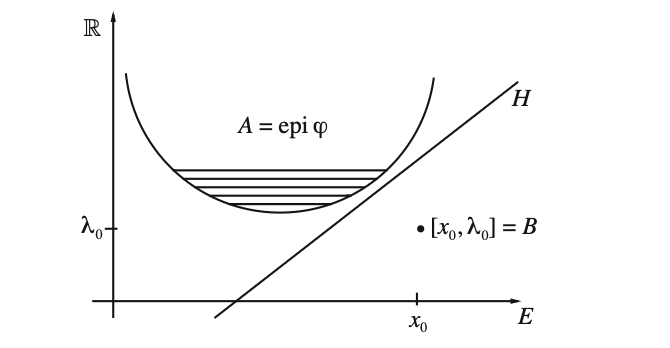
\includegraphics[width=0.48\textwidth]{fig2.png} % 图片宽度略小于环境宽度
    \end{figure}
    
    则
    \[
    \exists R \in \partial U, \text{ 使得 } r \text{ 通过 } R.
    \]
    容易看出 \( L(r) \geq L(\widehat{PR}) \geq L(\overline{C}) \)
\end{enumerate}
\end{proof}

\chapter{曲面的整体性质}
\section{测地三角形的Gauss公式}
\begin{figure}[h]
    \centering
    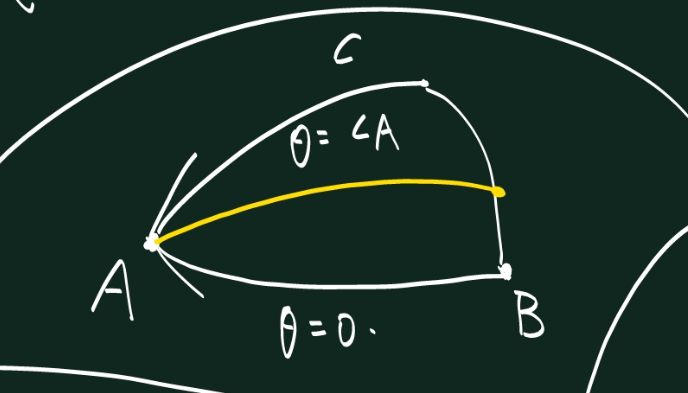
\includegraphics[width=0.48\textwidth]{fig3.png} % 图片宽度略小于环境宽度
\end{figure}
\begin{theorem}
    我们称 $\triangle ABC$ 为一个测地三角形,若
\begin{enumerate}
    \item 三条弧均存在于以 $A$ 为顶点的测地极坐标系中,且都是测地线。
    \item $\widehat{AB}$ 对应于 $\theta = 0$,$\widehat{AC}$ 对应于 $\theta = \angle A$。
    \item $\widehat{BC}$ 也是测地线。
\end{enumerate}

则
\[
\int_{\triangle ABC} K d\sigma = \angle A + \angle B + \angle C - \pi.
\]
\end{theorem}

\textbf{特例 1} 曲面为平面。
\[
K \equiv 0, \text{ 公式} \Leftrightarrow \angle A + \angle B + \angle C = \pi.
\]

\textbf{特例 2} 曲面为球面。
若半径为 \( R \),\( K = \frac{1}{R^2} \)。
\begin{figure}[h]
    \centering
    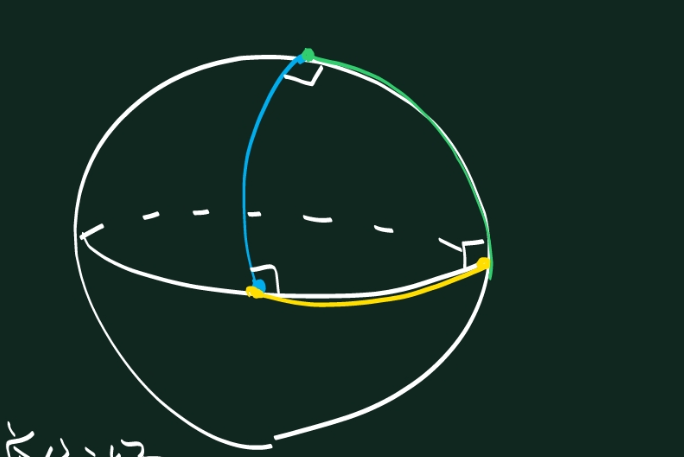
\includegraphics[width=0.48\textwidth]{fig4.png} % 图片宽度略小于环境宽度
\end{figure}

左
\[
 \int_{\triangle ABC} K d\sigma = \frac{1}{R^2} \int_{\triangle ABC} d\sigma = \frac{1}{R^2} S_{\triangle ABC}= \frac{1}{R^2} \cdot \frac{1}{2} (4\pi R^2) = \frac{\pi}{2}.
\]

右:\(\angle A + \angle B + \angle C - \pi = \pi\)($\angle A , \angle B ,  \angle $C都是 \(\pi/2\))。

\[
\angle A + \angle B + \angle C - \pi = \pi \Rightarrow \angle A + \angle B + \angle C - \pi = S_{\triangle ABC}.
\]
\begin{proof}
    注意到在测地极坐标系下,
\[
I = d\rho \otimes d\rho + G \, d\theta \otimes d\theta, \quad K = -\frac{(\sqrt{G})_{\rho\rho}}{\sqrt{G}}.
\]
\[
d\sigma = \sqrt{EG - F^2} \, d\rho \, d\theta = \sqrt{G} \, d\rho \, d\theta.
\]
故而 左边 \(= \int_{\triangle ABC} K \, d\sigma = \int_0^{\angle A} \left[ \int_0^{BC} -\frac{(\sqrt{G})_{\rho\rho}}{\sqrt{G}} \cdot \sqrt{G} \, d\rho \right] d\theta\)
\[
= \int_0^{\angle A} -(\sqrt{G})_{\rho \big|_{BC}} \bigg|_0^{\rho} \, d\theta. \quad (\text{注意到} \lim_{\rho \to 0} (\sqrt{G})_{\rho} = 1)
\]
\[
= \int_0^{\angle A} \left[ 1 - (\sqrt{G})_{\rho \big|_{BC}} \right] d\theta = \angle A - \int_0^{\angle A} (\sqrt{G})_{\rho \big|_{BC}} \, d\theta.
\]

\begin{wrapfigure}{r}{0.5\textwidth} % r: 图片右对齐;0.5\textwidth: 图片宽度
    \centering
    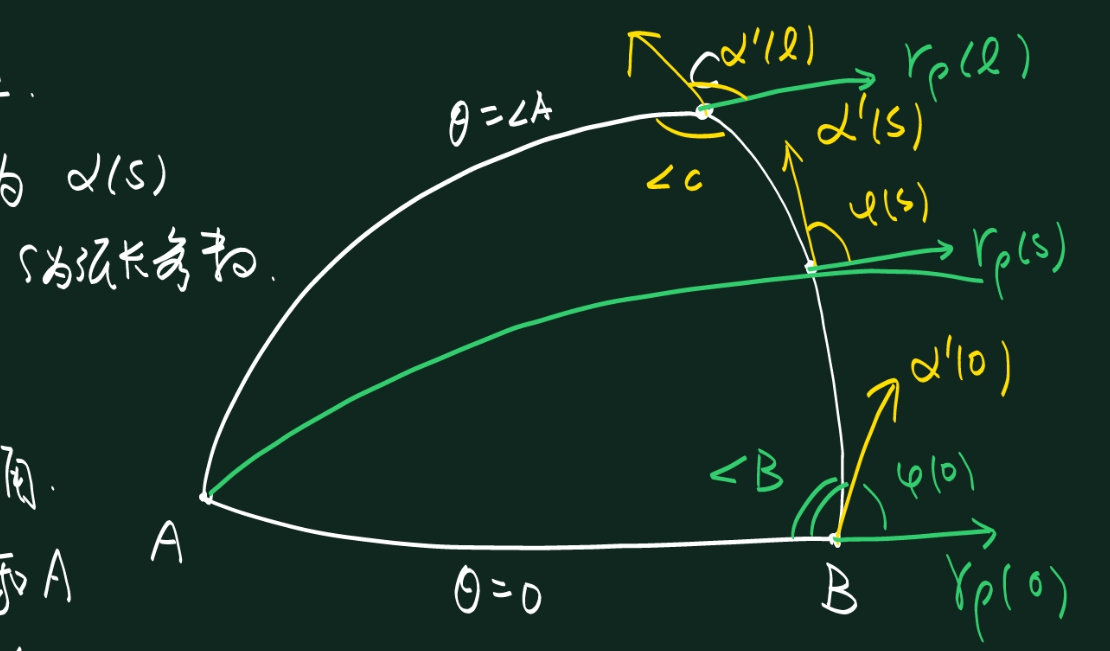
\includegraphics[width=0.48\textwidth]{fig5.png} % 图片宽度略小于环境宽度
   \end{wrapfigure}

  注意到 $\widehat{BC}$ 仍然在曲面上。

故而 $\widehat{BC}$ 可参数化为 $\alpha(s) = r(\rho(s), \theta(s))$。其中 $s$ 为弧长参数。

定义 $\varphi(s)$ 是 $\alpha'(s)$ 和 $\gamma_\rho(s)$ 的夹角。

其中 $r_\rho(s)$ 为 $\alpha(s)$ 和 $A$ 之间的 $\rho-$ 曲线的单位切向。

\textbf{FACT} 假设 $\widehat{BC}$ 弧长为 $\ell$.

\begin{enumerate}
    \item $\varphi(0) = \pi - \angle B.$
    \item $\varphi(\ell) = \angle C.$
    \item $\varphi$ 关于 $S$ 可微
    \item $\cos \varphi(s) = \alpha'(s) \cdot \gamma_{\rho}(s)$
    \item $\sin \varphi(s) = \alpha'(s) \cdot \gamma_{\theta}(s) / \sqrt{g}.$
\end{enumerate}
故下证
\[
\int_0^{\angle A}   - (\sqrt{G})_{\rho}  \bigg|_{BC} d\theta = \int_0^{\ell} -(\sqrt{G})_ {\rho} \frac{d\theta}{ds} ds = \int_0^{\ell} \frac{d\varphi}{ds} ds \tag{*}
\]

对(4)关于 $s$ 求导
\begin{align*}
    -\sin \varphi(s) \cdot \frac{d\varphi}{ds} &= \alpha'(s) \cdot r_{\rho}(s) + \alpha'(s) \cdot \frac{d}{ds} r_{\rho}(s).\\
    &= \alpha'(s) \cdot \frac{d}{ds} r_{\rho}(\rho(s), \theta(s))\\
    &=\left( r_{\rho} \frac{d\rho}{ds} + r_{\theta} \frac{d\theta}{ds} \right) \cdot \left( r_{\rho\rho} \frac{d\rho}{ds} + r_{\rho\theta} \frac{d\theta}{ds} \right).
\end{align*}


注意到$\quad |r_\rho| = 1 \iff r_\rho \cdot r_\rho = 1 \Rightarrow 
\begin{cases}
r_\rho \cdot r_{\rho\rho} = 0 \\
r_\rho \cdot r_{\rho\theta} = 0
\end{cases}$
\[
r_\theta \cdot r_{\rho\rho} = (r_\theta \cdot r_\rho)_{\rho\rho} - r_{\rho\theta} \cdot r_\rho = 0
\]

\[
\Rightarrow -\sin\varphi(s) \frac{d^2 \varphi}{ds^2} = r_\theta \cdot r_\rho \left( \frac{d\theta}{ds} \right)^2 = \frac{1}{2} G_\rho \left( \frac{d\theta}{ds} \right)^2
\]

\[
\text{但同时} \quad \sin\varphi(s) = \alpha'(s) \cdot \frac{r_\theta}{\sqrt{G}} = \left( r_\rho \frac{d\rho}{ds} + r_\theta \frac{d\theta}{ds} \right) \cdot \frac{r_\theta}{\sqrt{G}} = \sqrt{G} \left( \frac{d\theta}{ds} \right)
\]

\[
\Rightarrow \frac{d\varphi}{ds} = -\frac{G_\rho}{2\sqrt{G}} \left( \frac{d\theta}{ds} \right) = -\left( \sqrt{G} \right)_\rho \left( \frac{d\theta}{ds} \right)
\]
回带*即可证得


\end{proof}
\begin{remark}
    事实上 Gauss 测地三角形公式的 $\angle A, \angle B, \angle C$ 相应换成外角.
\end{remark}
\begin{definition}[外角]
    记
$$
\begin{cases}
\theta_1 = \pi - \angle A \\
\theta_2 = \pi - \angle B \\
\theta_3 = \pi - \angle C
\end{cases}
\quad \text{为对应的外角.}
$$
\end{definition}
公式改写为
\begin{align*}
\int_{\triangle ABC} K d\sigma &= \angle A + \angle B + \angle C - \pi \\
&= (\pi - \theta_1) + (\pi - \theta_2) + (\pi - \theta_3) - \pi
\end{align*}

$$
\iff \boxed{\int_{\triangle ABC} K d\sigma + \sum_{i=1}^{3} \theta_i = 2\pi}
$$

\begin{remark}
    平面三角形的内角和为$\pi$是"偶然"的.

四边形内角和 $\to 2\pi$

$n$边形内角和 $\to (n-2)\pi$

但所有$n$边形外角和总是 $n\pi - (n-2)\pi = 2\pi$.

故而 Gauss 定理是在说
$$ \int_{\triangle ABC} K d\sigma + \text{外角和} = 2\pi. $$
\end{remark}

我们想推广 Gauss 定理到多边形.
\begin{definition}[分段光滑简单闭合曲线)]
    $$ \alpha: [0, l] \to S $$
连续曲线满足:
\begin{enumerate}
    \item $\alpha(0) = \alpha(l)$
    \item 若 $S_1 \neq S_2$, $S_1, S_2 \in [0, l)$, 则 $\alpha(S_1) \neq \alpha(S_2)$
    \item 存在一个 $[0, l]$ 的分割 $0=t_0 < \dots < t_k = l$, 使得 $\alpha(t)$ 在 $[t_{i-1}, t_i]$ 上都光滑. (即 $t=t_i$ 处可能有外角)
\end{enumerate}
\end{definition}
\begin{figure}[h]
    \centering
    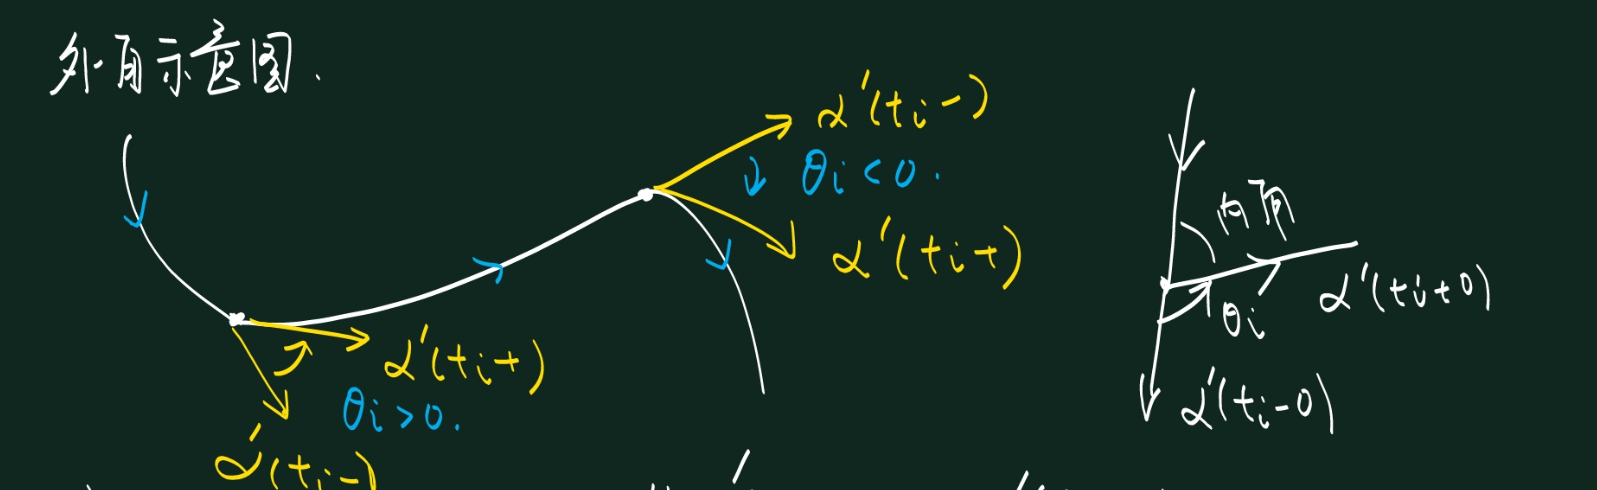
\includegraphics[width=0.6\textwidth]{fig6.png} % 图片宽度略小于环境宽度
\end{figure}
\begin{definition}[外角]
    我们规定,若 $\alpha'(t_i-0) \ne \alpha'(t_i+0)$,从 $\alpha'(t_i-0)$ 到 $\alpha'(t_i+0)$ 逆时针定向成外角 $\theta_i$.

\textbullet \ $-\pi \le \theta_i \le \pi$. (对于三角形外角的一种推广).
\end{definition}

Bonnet 推广了 Gauss 定理, 将其中测地线的要求去掉!
\section{Gauss - Bonnet 定理, 局部版本}
\begin{theorem}
    假设 $C$ 为曲面 $S$ 上一条分段光滑、简单闭曲线,
其所围成的区域为 $D$, $C$ 上的外角记为 $\theta_i$, 则
$$ \iint_D K d\sigma + \oint_C k_g ds + \sum_{i=1}^n \theta_i = 2\pi. $$
\end{theorem}
\end{document}
